%!TEX root=./LIVRO.tex
\setcounter{chapter}{0}
\chapter[Simulado 1]{Simulado}
\markboth{Simulado 1}{}

\num{1} Veja o número que aparece na porta de entrada da casa e indique o que
ele representa.

\begin{figure}[H]
\centering
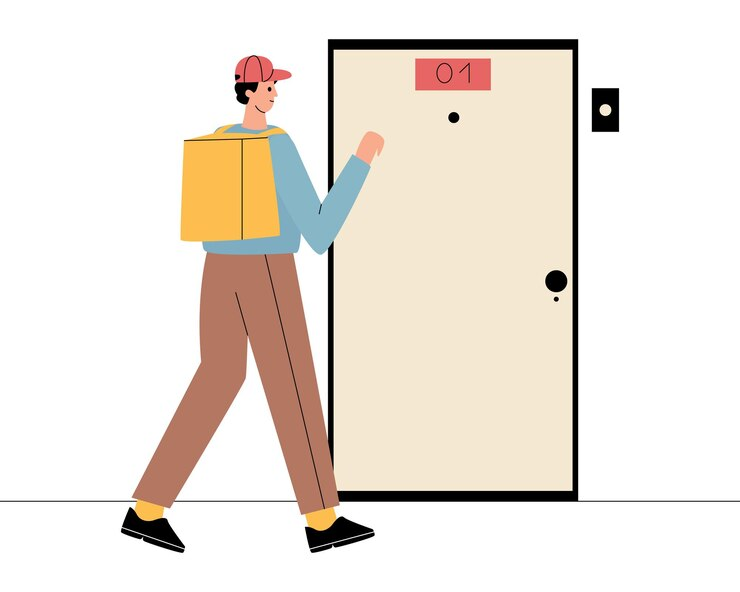
\includegraphics[width=.6\textwidth]{./media/image105old.png}
\end{figure}

%\textless{} Https://br.Freepik.Com/vetores-premium/um-mensageiro-entrega-um-pacote-no-endereco-o-mensageiro-esta-na-porta\_21480220.Htm\#page=4\&query=port\%c3\%a3o\%20entregador\&position=8\&from\_view=search\&track=ais \textgreater{}

\begin{escolha}[itemsep=-5pt]
\begin{multicols}{2}
\item Código de identificação.

\item Medida.

\item Ordem.

\item Quantidade.
\end{multicols}
\end{escolha}

\num{2} Analise a fila de atendimento de um banco. Qual é o nome da pessoa que
está na segunda posição dessa fila?

\begin{figure}[H]
\centering
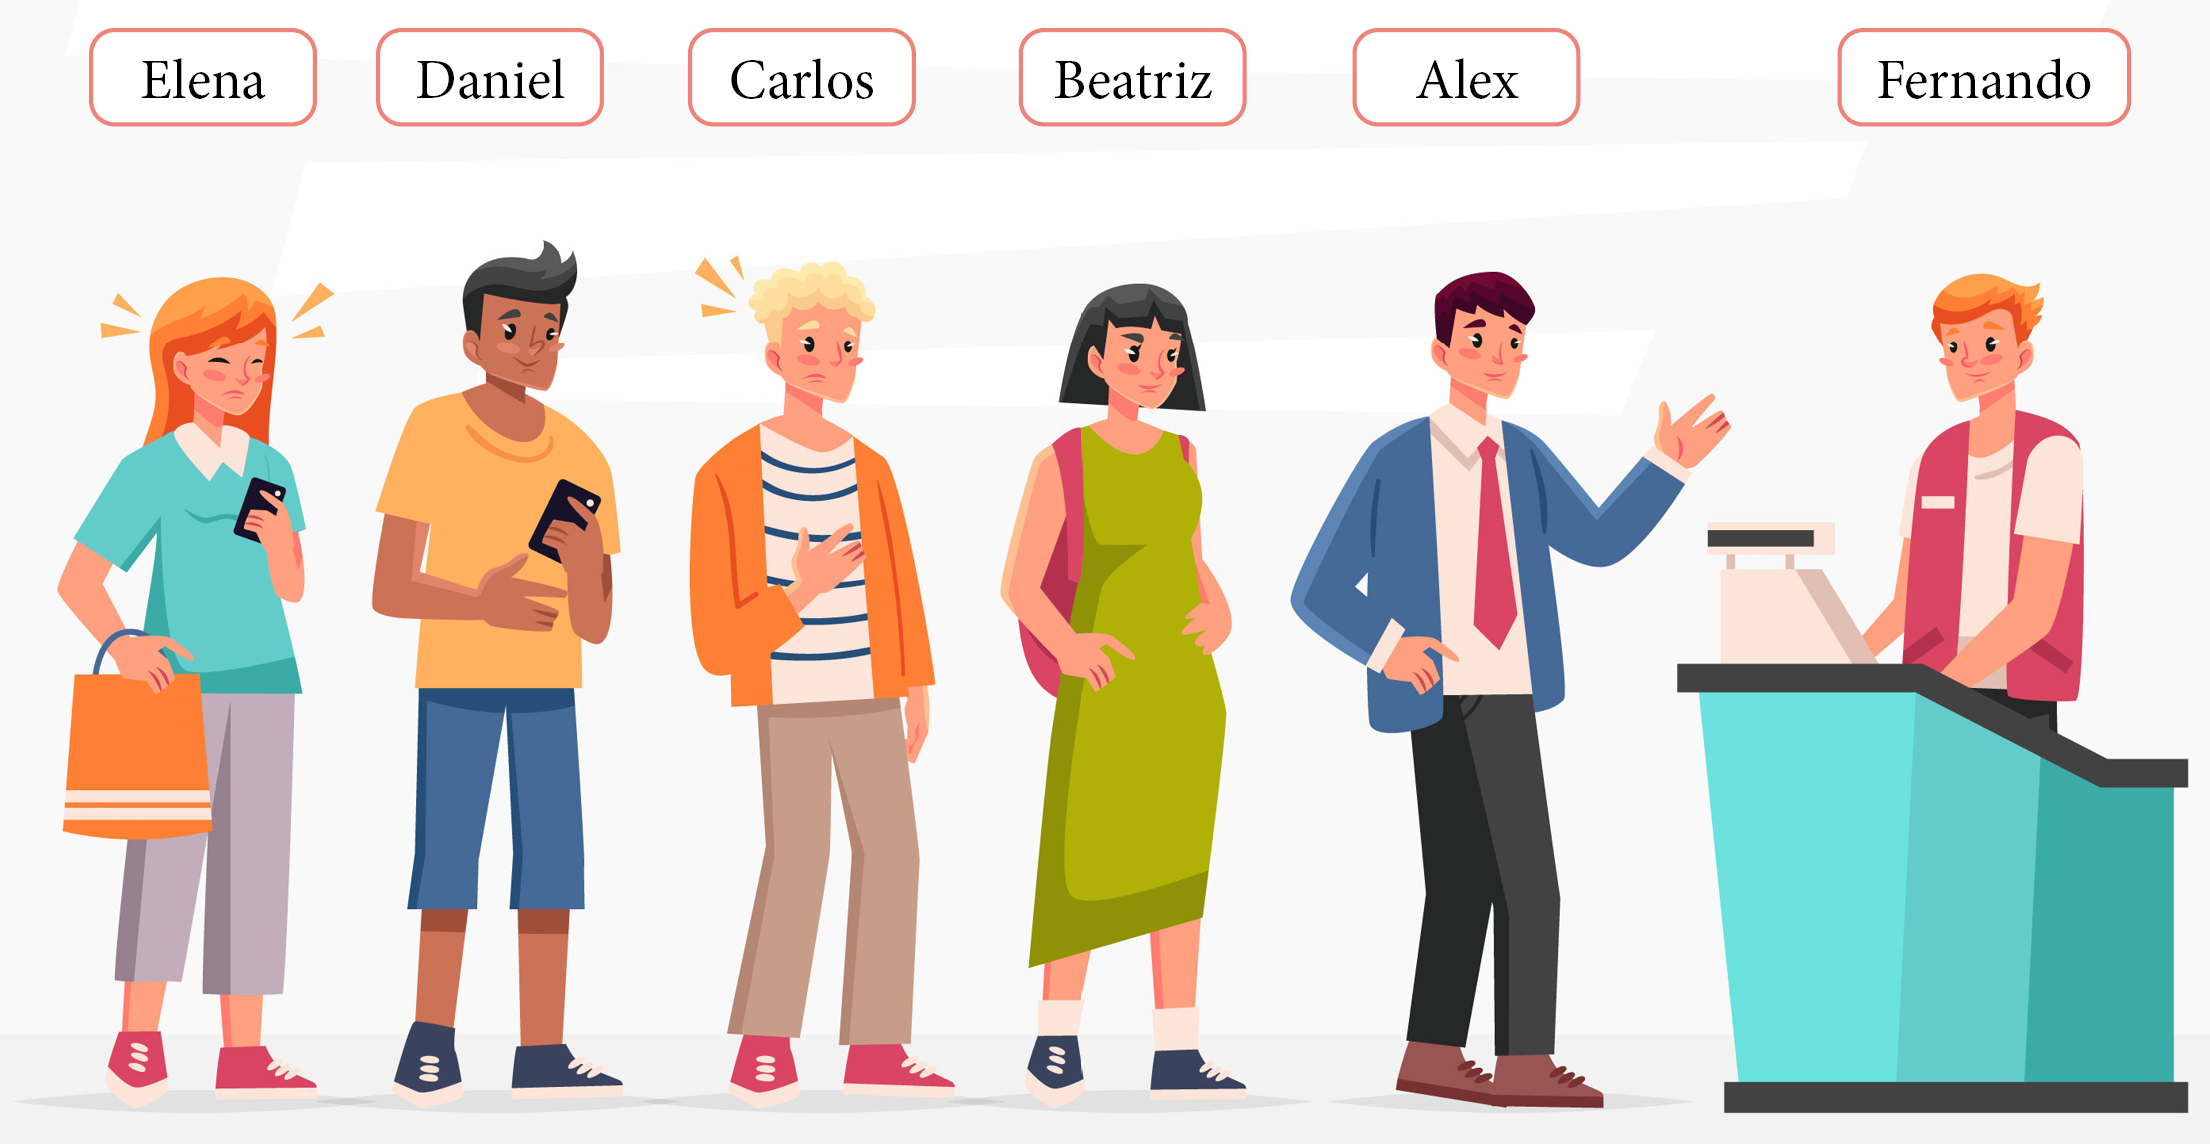
\includegraphics[width=.8\textwidth]{./media/image113.png}
\end{figure}

\begin{escolha}[itemsep=-5pt]
\begin{multicols}{2}
\item Alex.

\item Beatriz.

\item Carlos.

\item Daniel.
\end{multicols}
\end{escolha}

\pagebreak

\num{3} Adicione 45 a 75 e depois subtraia 15. Indique o resultado correto.

\begin{escolha}[itemsep=-5pt]
\item 95

\item 105

\item 110

\item 120
\end{escolha}

\num{4} Yasmim comprou um sapato no valor de 175 reais. Marque a alternativa que apresenta uma combinação de cédulas que componham o preço do sapato.

\begin{figure}[H]
\centering
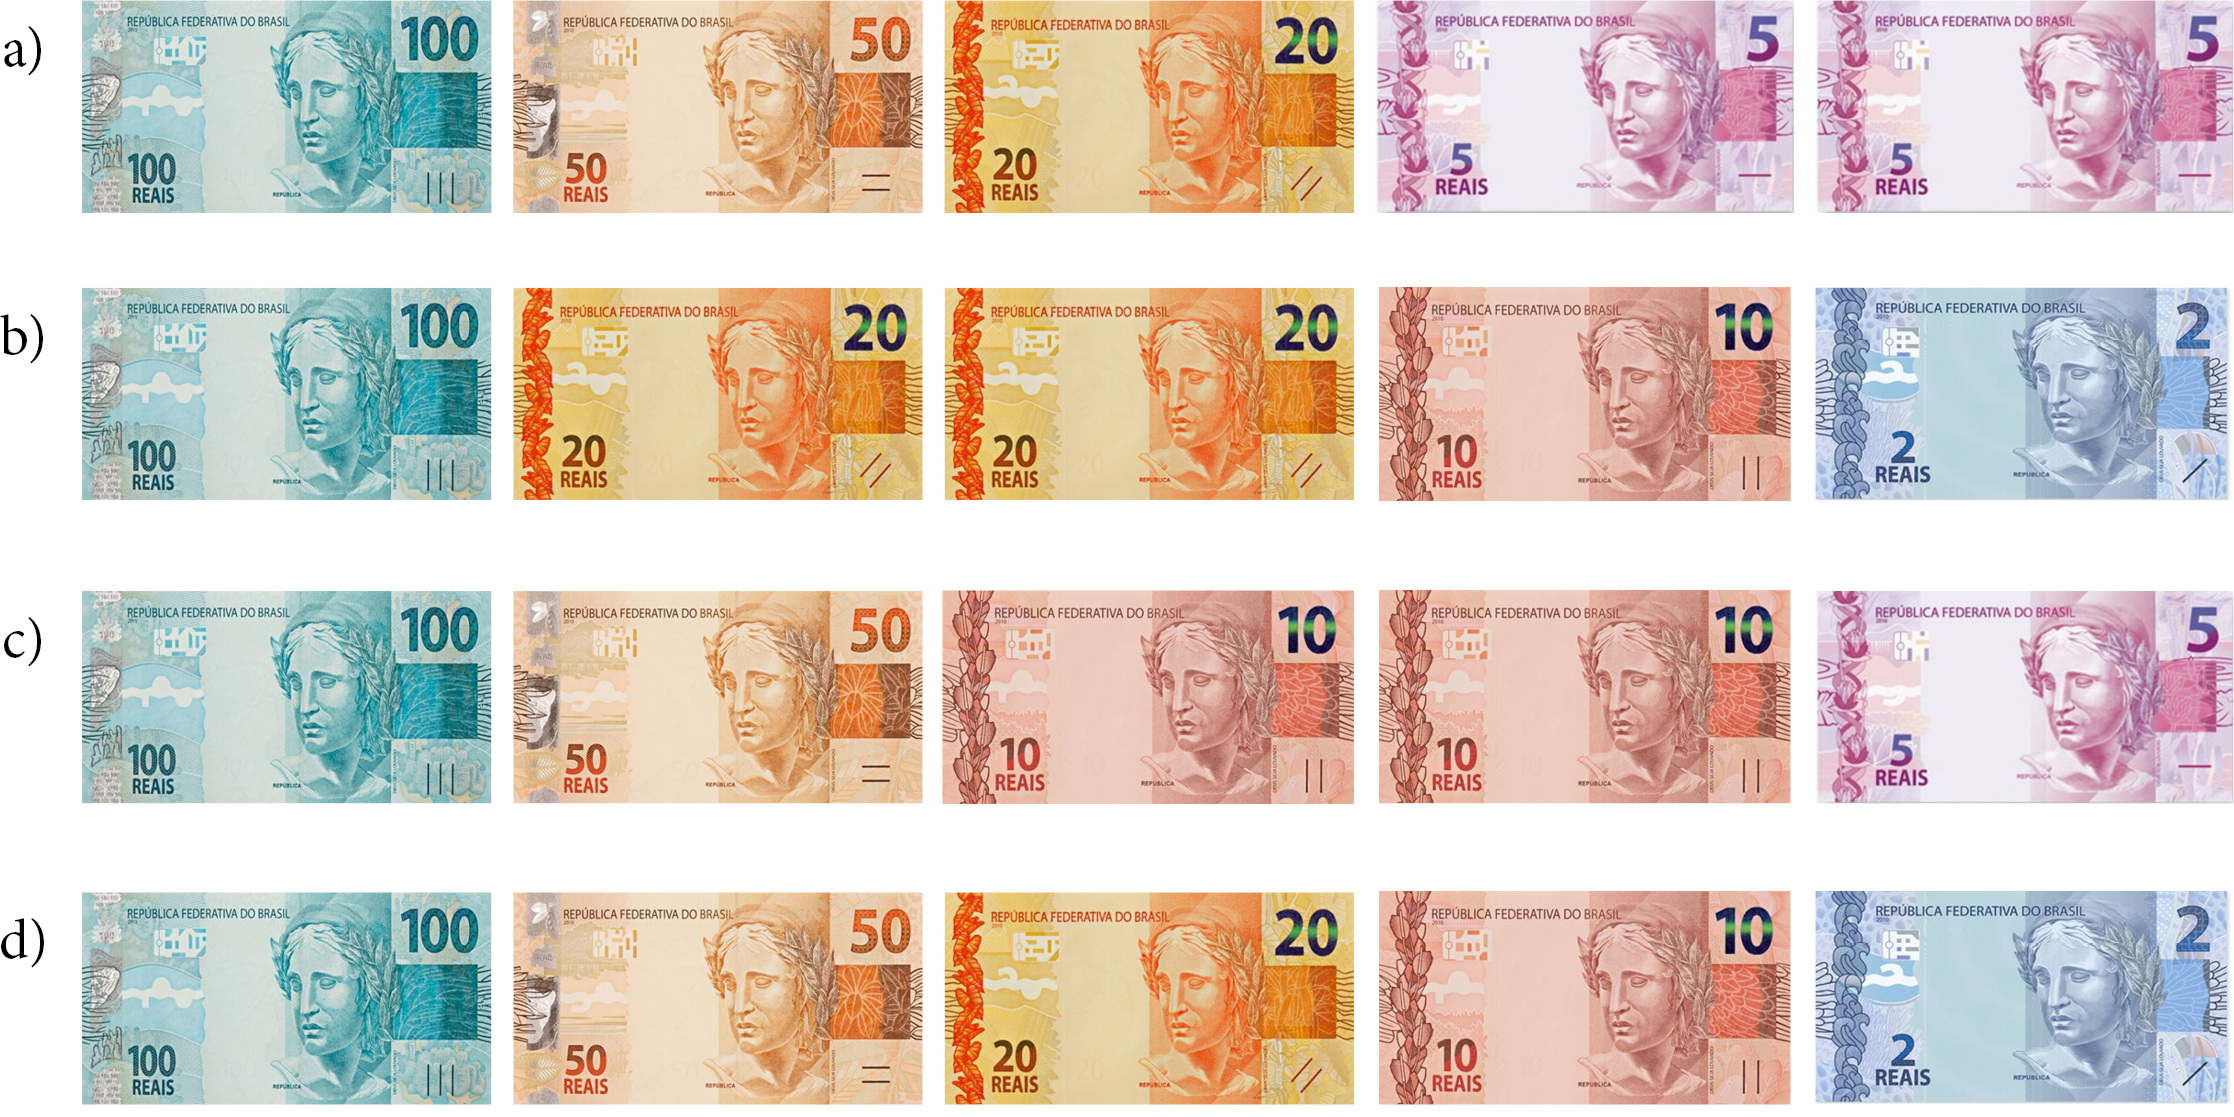
\includegraphics[width=\textwidth]{./media/image115.png}
\end{figure}

\num{5} Observe a imagem. Qual é o maior número possível de se formar com os
algarismos sem repeti-los?

\begin{figure}[H]
\centering
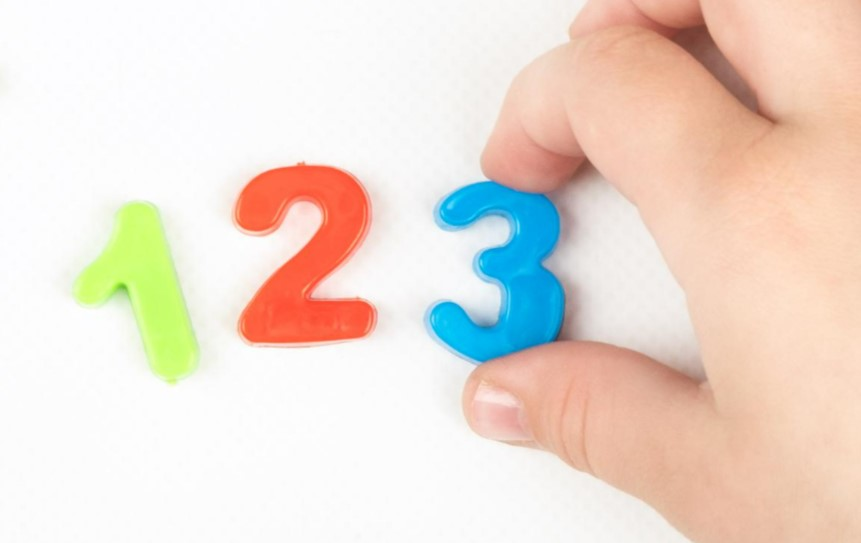
\includegraphics[width=.6\textwidth]{./media/image114.png}
\end{figure}

\begin{escolha}[itemsep=-5pt]
\item 123

\item 231

\item 312

\item 321
\end{escolha}

\num{6} Observe alguns animais da fazenda do Osvaldo e marque a afirmação correta.

\begin{figure}[H]
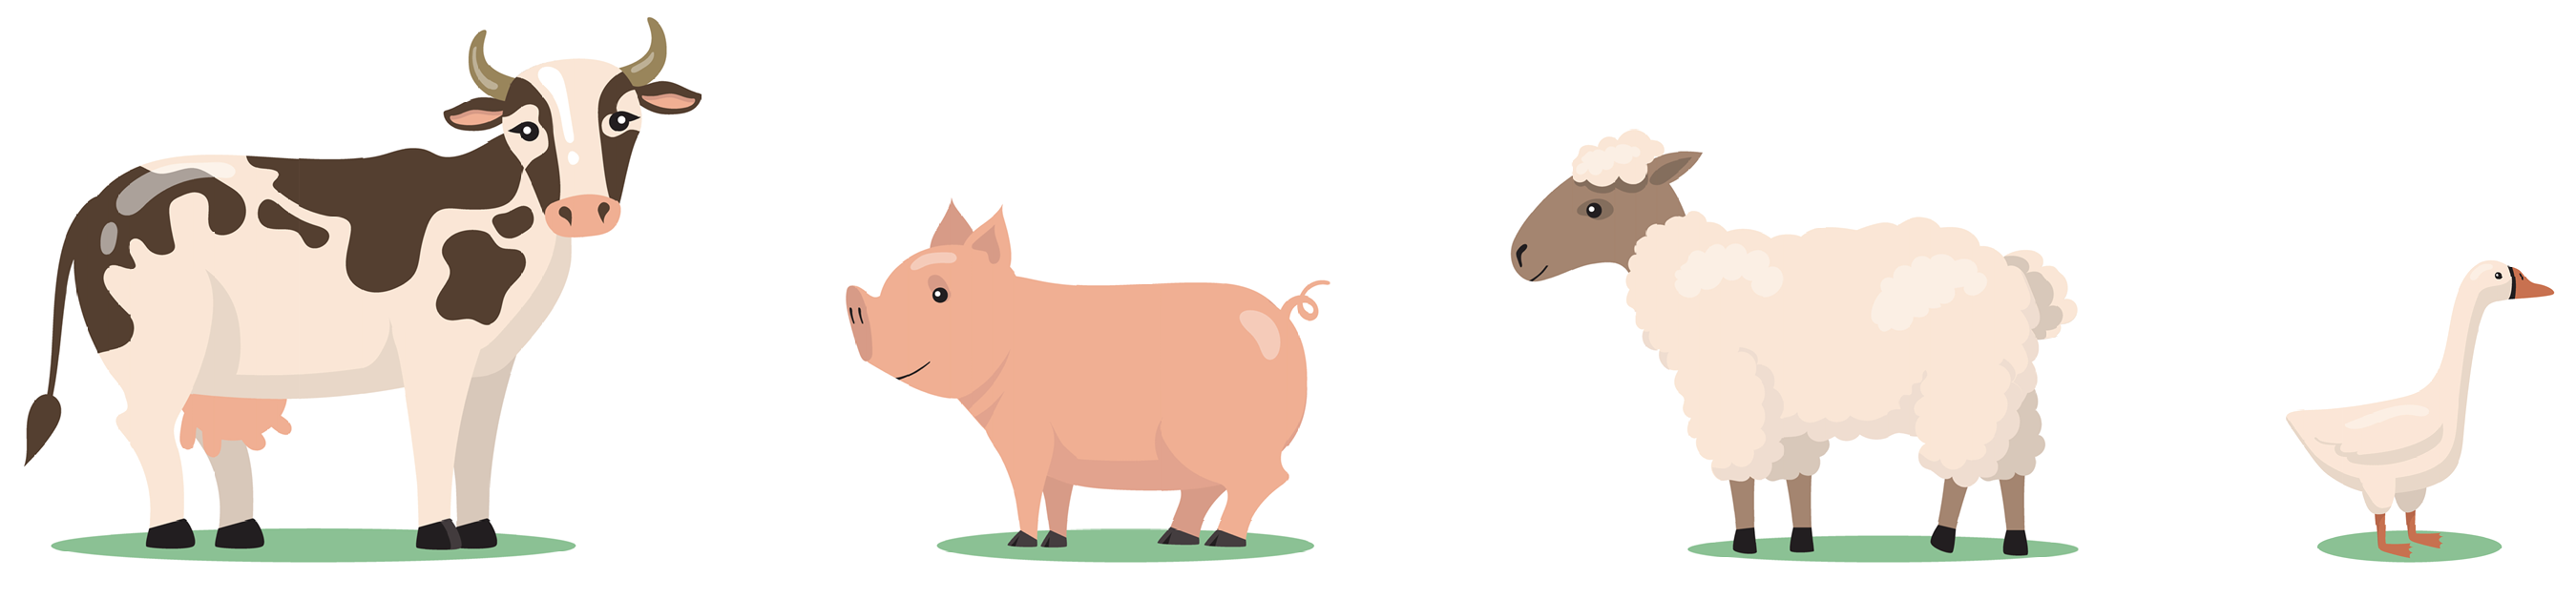
\includegraphics[width=.8\textwidth]{./media/image116.png}
\end{figure}

%\textless{}Criar figuras conforme modelo. Utilizar como referência: \url{https://br.freepik.com/vetores-gratis/varios-animais-e-animais-de-estimacao-no-conjunto-de-clipart-plana-de-fazenda-personagens-de-desenhos-animados-de-colecao-de-ilustracao-vetorial-isolado-de-cavalo-ovelha-porco-cabra-ganso-e-burro_10173994.htm}\textgreater{}

\begin{escolha}[itemsep=-5pt]
\item A ovelha é o animal mais baixo.

\item A vaca é o animal mais pesado.

\item O pato é o animal mais alto.

\item O porco é o animal mais leve.
\end{escolha}

\num{7} Mariana observou que 5 passos seus equivalem a 1 metro e que há uma
distância de 40 passos da porta de sua casa até a porta da casa de sua vizinha. Qual é essa distância em metros?

\begin{figure}[H]
\centering
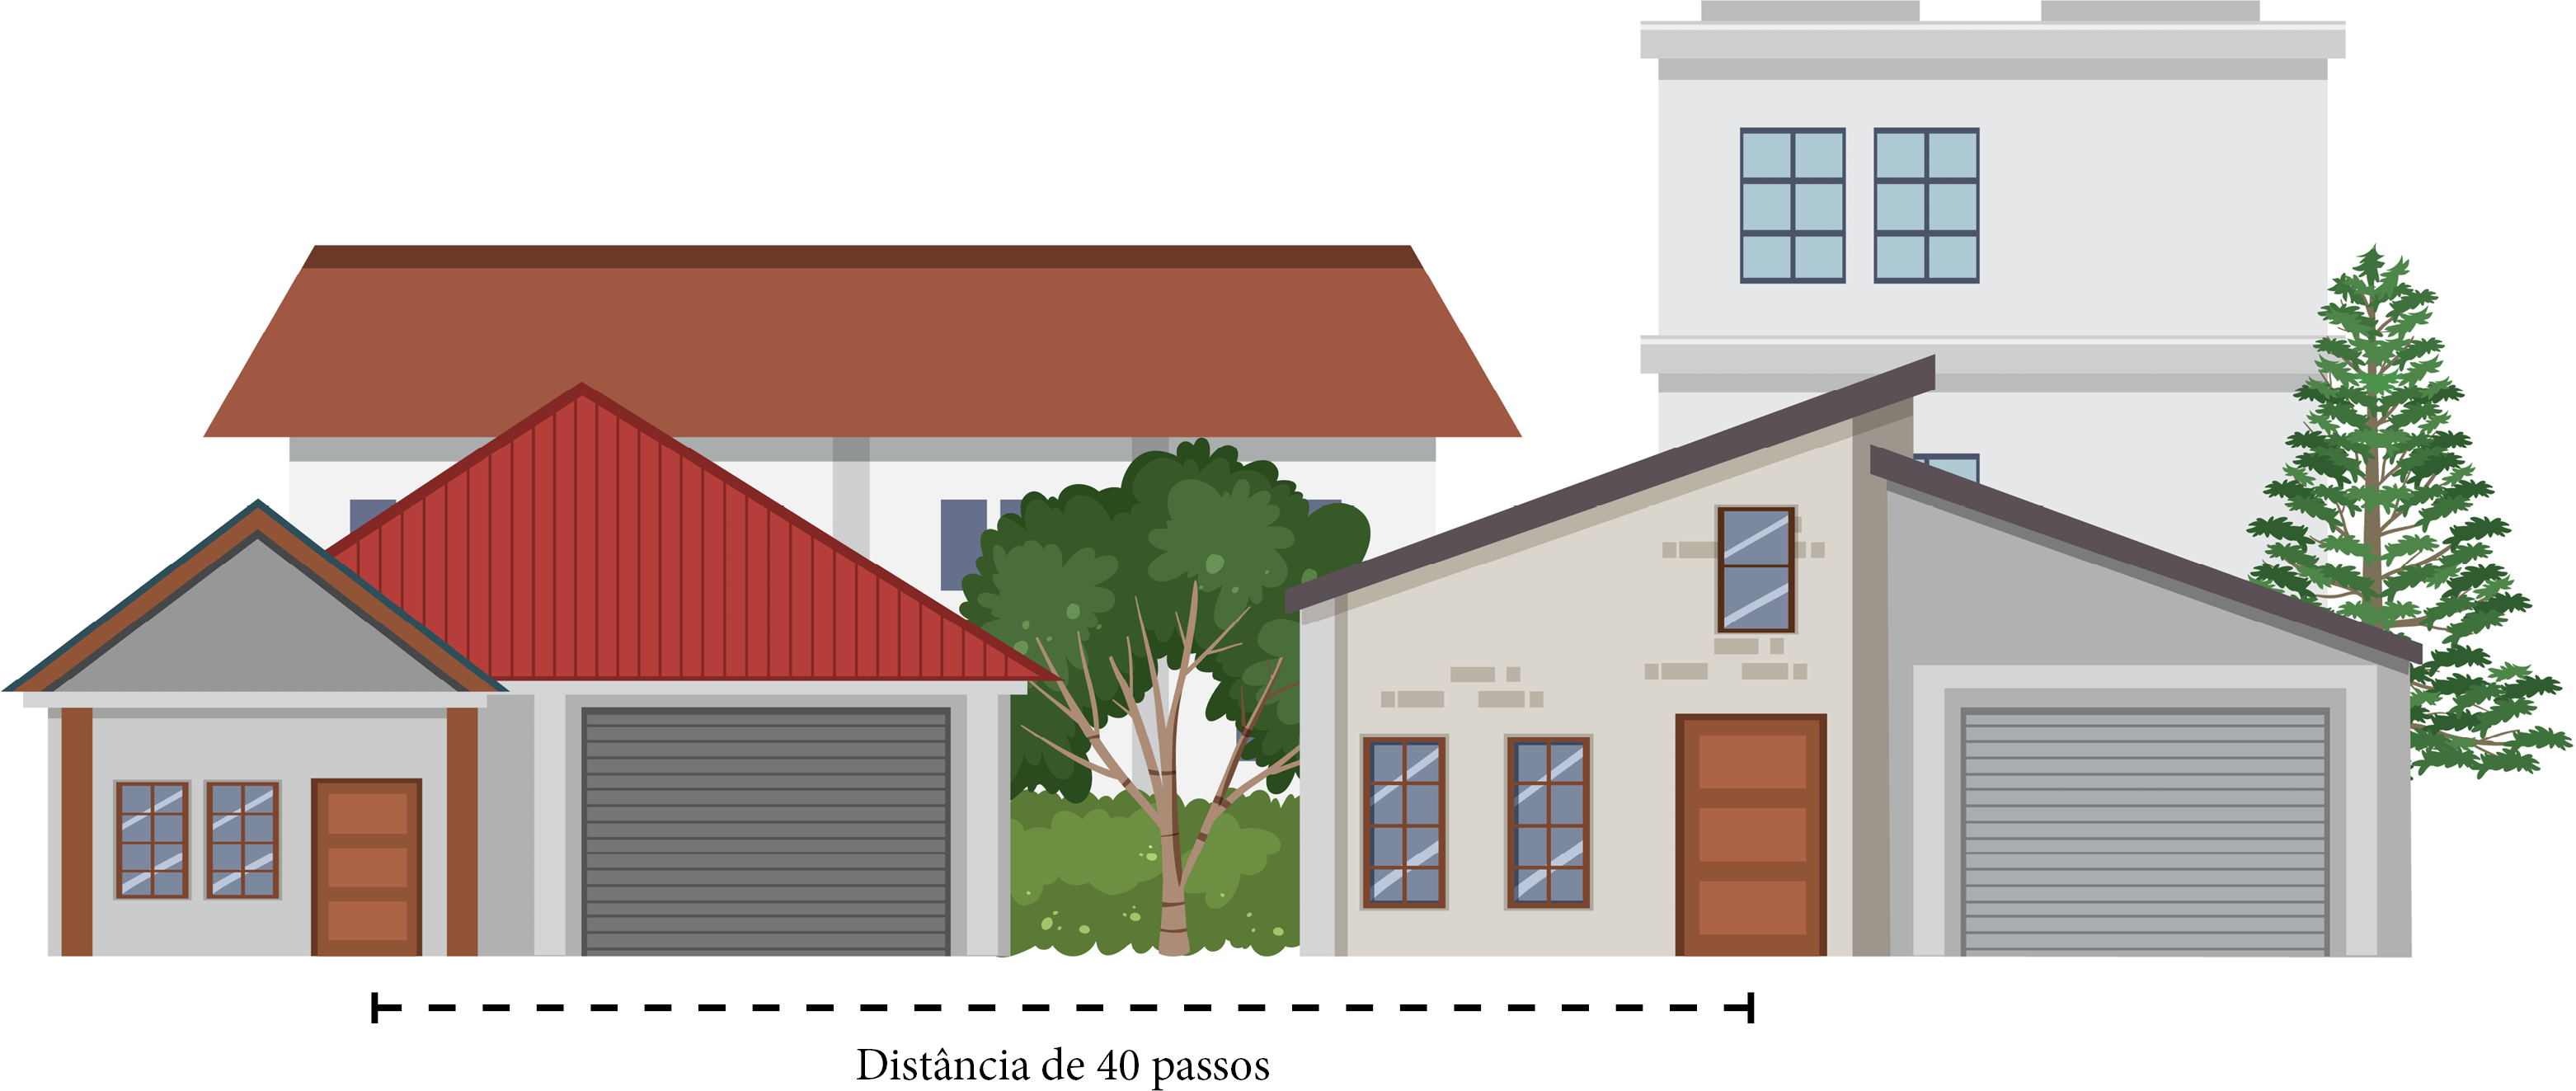
\includegraphics[width=.8\textwidth]{./media/image117.png}
\end{figure}

\begin{escolha}[itemsep=-5pt]
\begin{multicols}{2}
\item 5 metros.

\item 6 metros.

\item 7 metros.

\item 8 metros.
\end{multicols}
\end{escolha}

\num{8} Observe a rotina de Daniel e marque a alternativa correta.

\begin{figure}[H]
\centering
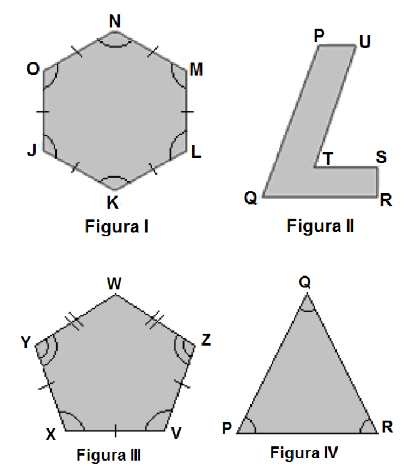
\includegraphics[width=\textwidth]{./media/image118.png}
\end{figure}

\begin{escolha}[itemsep=-5pt]
\item Ele acorda às 6 horas da manhã. Entre o horário de acordar e o horário de trabalhar passam-se dez horas.

\item Ele toma banho às 10 horas da noite. Entre o horário de trabalhar e o horário de tomar banho passam-se duas horas.

\item Ele faz o lanche da tarde às 3 horas. Entre o horário de lanchar e o horário de tomar banho passam-se seis horas.

\item Ele trabalha às 8 horas da noite. Entre o horário de acordar e o horário de lanchar passam-se cinco horas.
\end{escolha}

\num{9} Observe o calendário e responda: se Carla sempre vai ao mercado na
quinta-feira e, em determinada semana, caiu no dia 17, em qual dia caiu na semana anterior?

\begin{figure}[H]
\centering
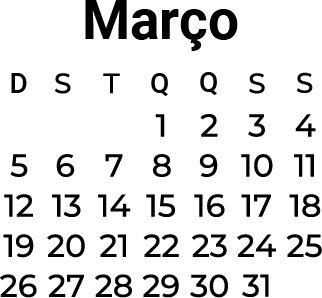
\includegraphics[width=.5\textwidth]{./media/image119.png}
\end{figure}

\begin{escolha}[itemsep=-5pt]
\item 3

\item 10

\item 24

\item 31
\end{escolha}

\num{10} Gabriela pegou o molho de chaves de sua mãe para abrir o portão da
garagem. Porém, ela não sabe qual das 5 chaves é a correta; somente uma
delas abre o portão. Então podemos dizer que

\begin{escolha}[itemsep=-5pt]
\item é muito provável que Gabriela consiga abrir o portão na primeira tentativa.

\item é provável que Gabriela consiga abrir o portão na primeira tentativa.

\item é pouco provável que Gabriela consiga abrir o portão na primeira tentativa.

\item é impossível que Gabriela consiga abrir o portão na primeira tentativa.
\end{escolha}

\num{11} Joaquim quer uma bola nova e, para comprá-la, pegou as economias do
seu cofrinho. Observe as moedas e indique o valor que ele tem para comprar a bola.

\begin{figure}[H]
\centering
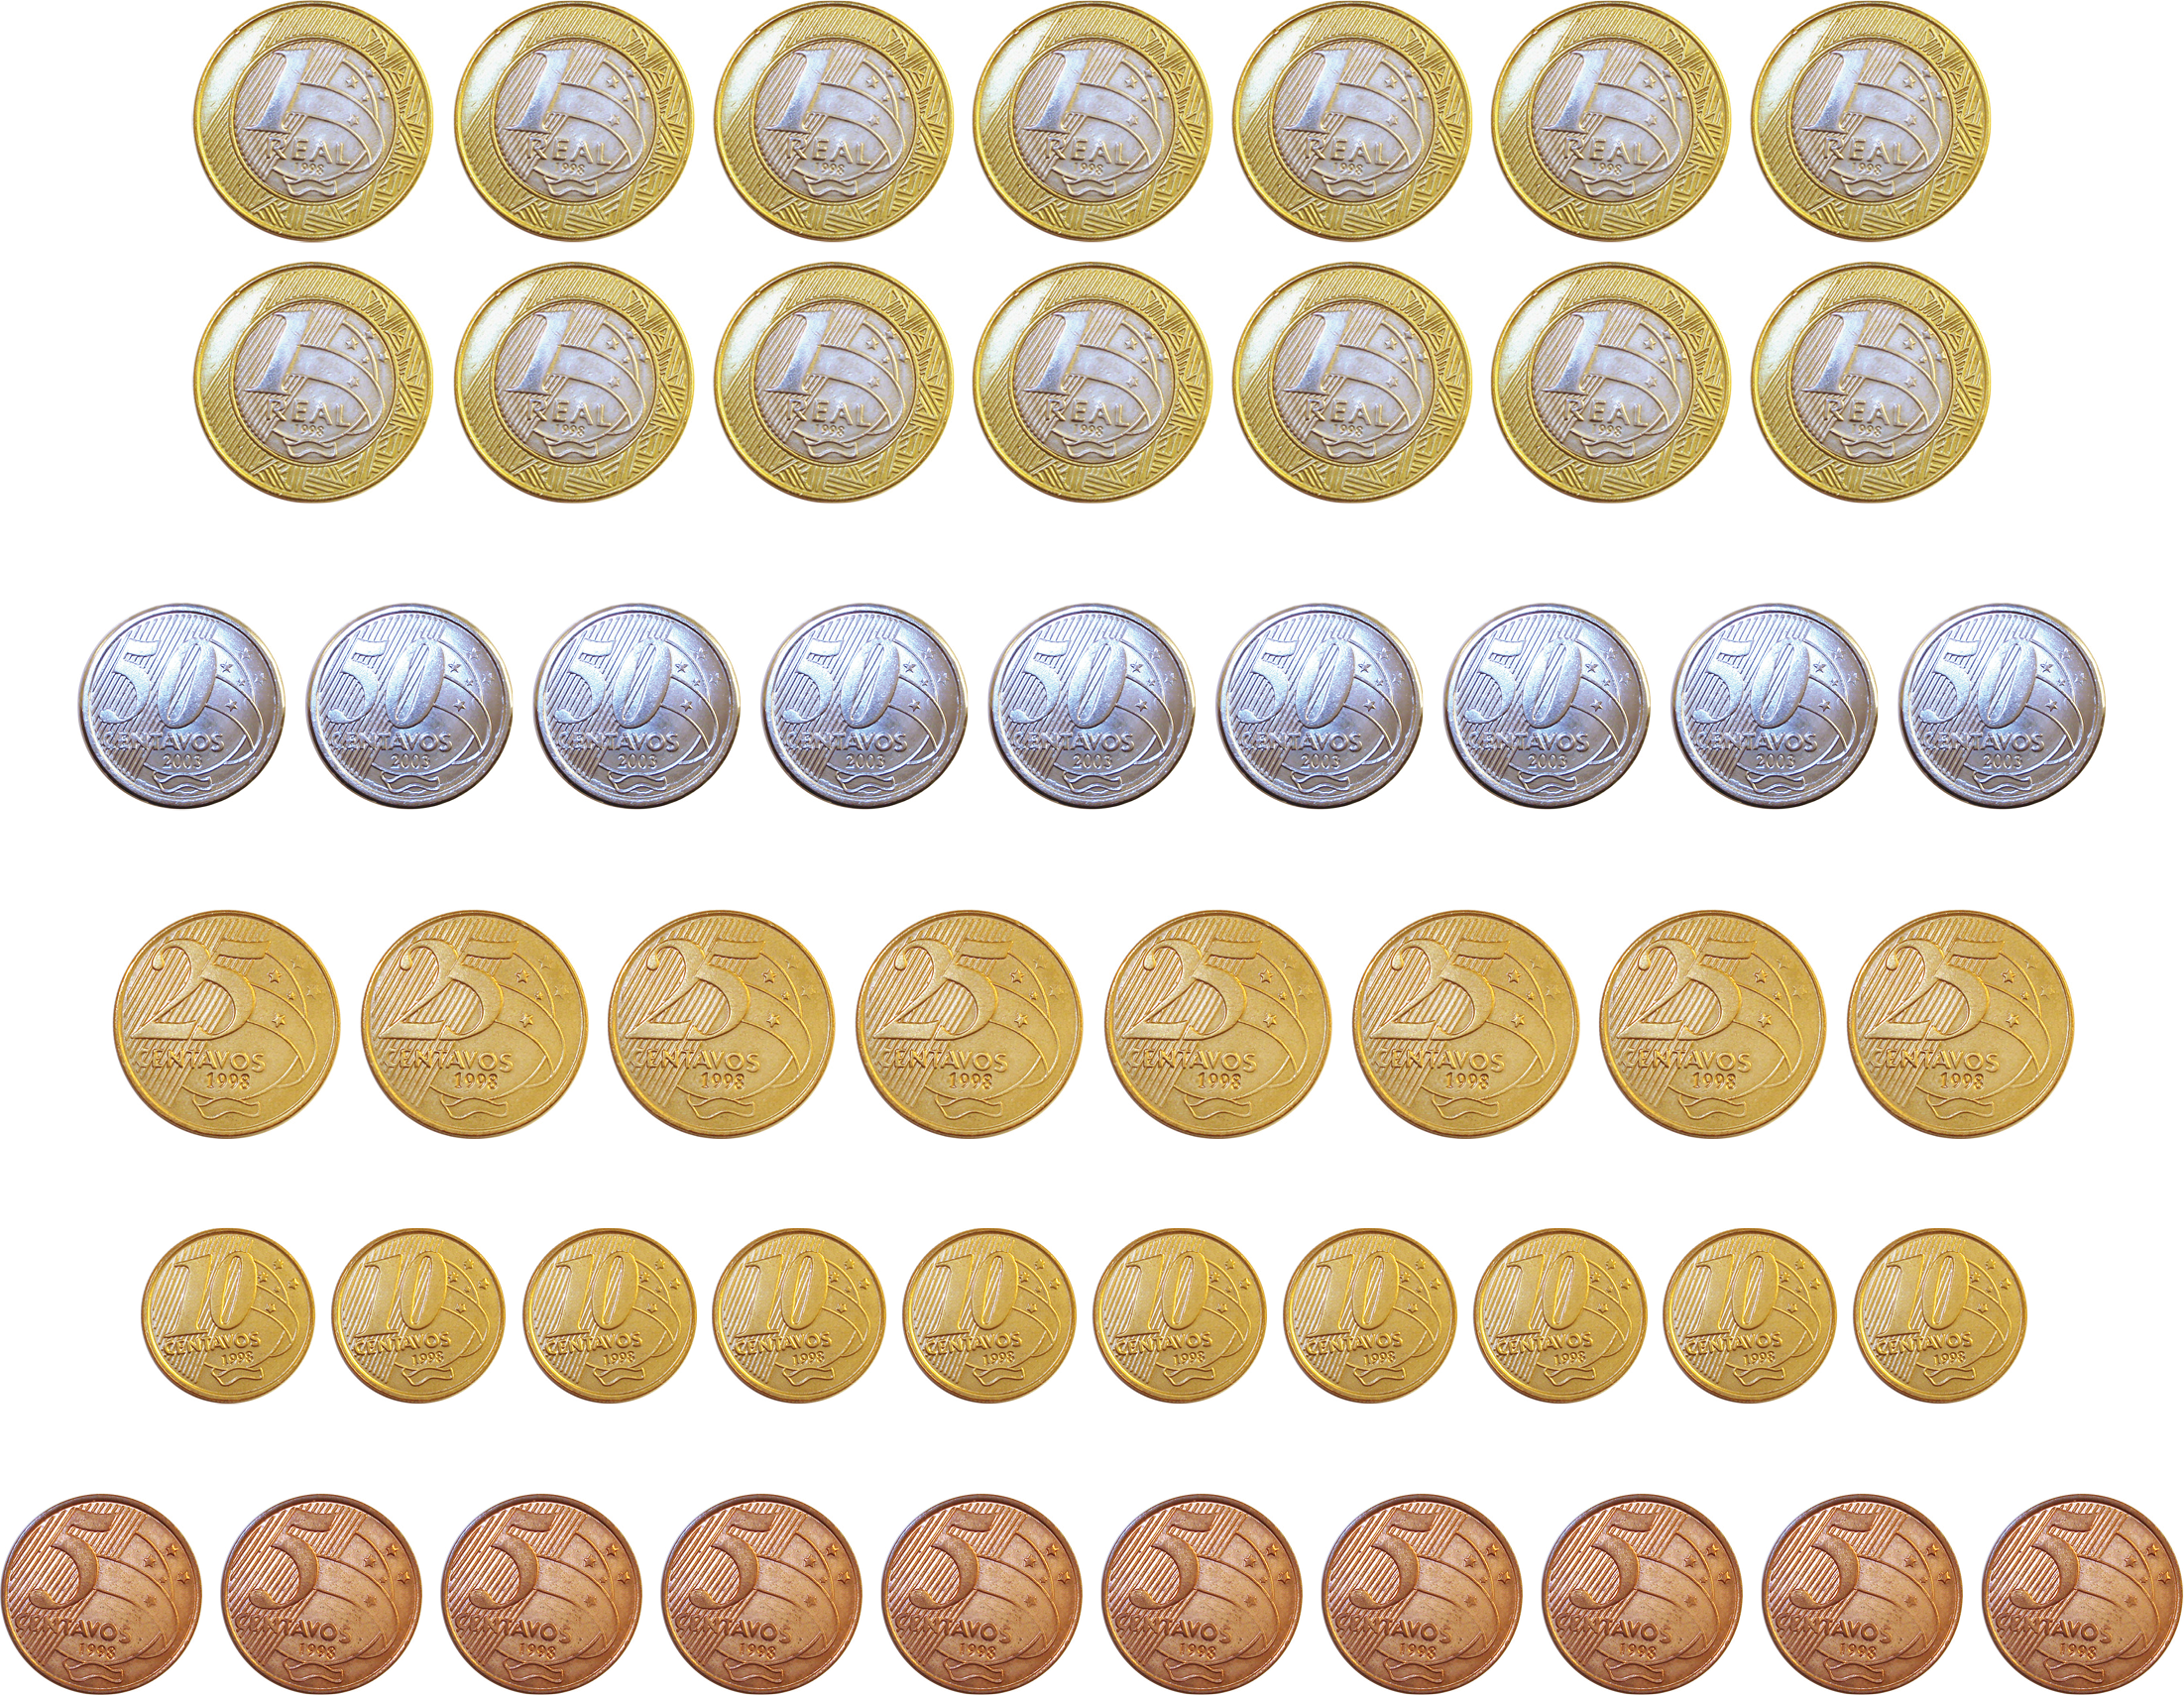
\includegraphics[width=.8\textwidth]{./media/image120.png}
\end{figure}

\begin{escolha}[itemsep=-5pt]
\item 21 reais e 50 centavos.

\item 22 reais.

\item 22 reais e 50 centavos.

\item 23 reais.
\end{escolha}

\num{12} Taís foi ao Parque de Diversões com mais 3 amigas e pagou todos os ingressos. Marque a afirmativa correta sobre o valor total que ela pagou.

\begin{escolha}[itemsep=-5pt]
\item Ela pagou a terça parte do valor do ingresso.

\item Ela pagou o dobro do valor do ingresso.

\item Ela pagou o triplo do valor do ingresso.

\item Ela pagou quatro vezes o valor do ingresso.
\end{escolha}

\num{13} Alana, Bruno, Carla e Denílson estão brincando de um jogo em que o
jogador que fizer mais pontos vence. Observe a tabela com os pontos de
cada um e responda quem foi o(a) ganhador(a) da brincadeira.

\begin{figure}[H]
\centering
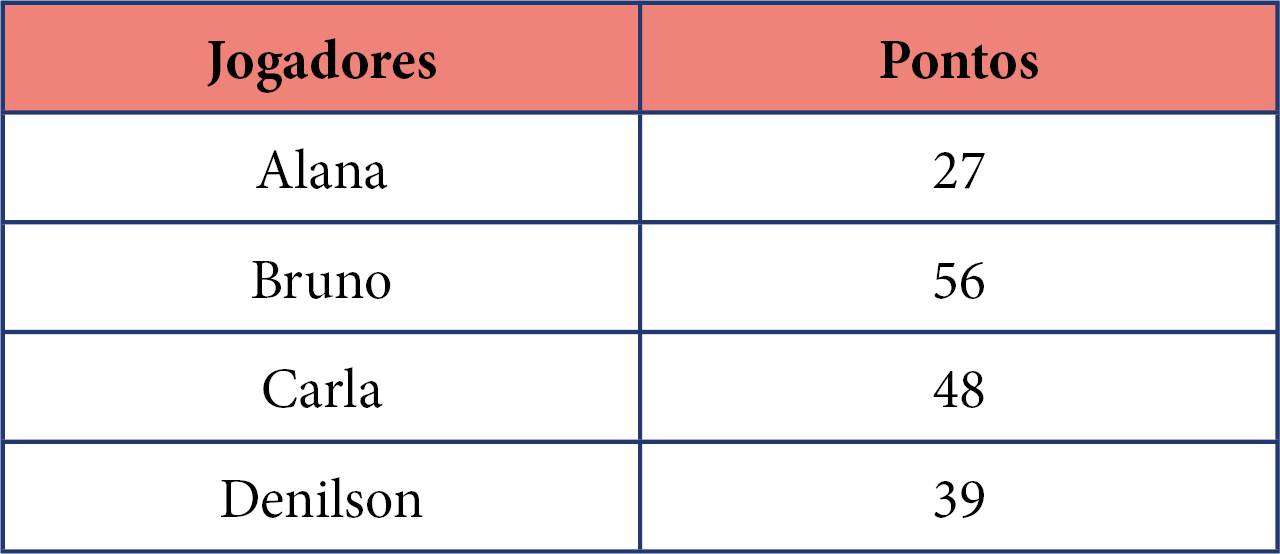
\includegraphics[width=.7\textwidth]{./media/image121.png}
\end{figure}

\begin{escolha}[itemsep=-5pt]
\item Alana.

\item Bruno.

\item Carla.

\item Denílson.
\end{escolha}

\num{14} Wendel tem 2 pilhas de livros e cada uma delas possui 12 livros. Quantos livros ele tem ao todo?

\begin{figure}[H]
\centering

\includegraphics[width=.5\textwidth]{./media/image177.jpg}
\end{figure}

\begin{escolha}[itemsep=-5pt]
\begin{multicols}{2}
\item 20

\item 22

\item 24

\item 26
\end{multicols}
\end{escolha}

\num{15} A Prefeitura de Luziânia irá construir uma quadra de esportes no bairro
Estrela Dalva e, para incluir os elementos certos no projeto, fez uma
pesquisa para saber os esportes de preferência entre os moradores
do bairro.

\begin{figure}[H]
\centering
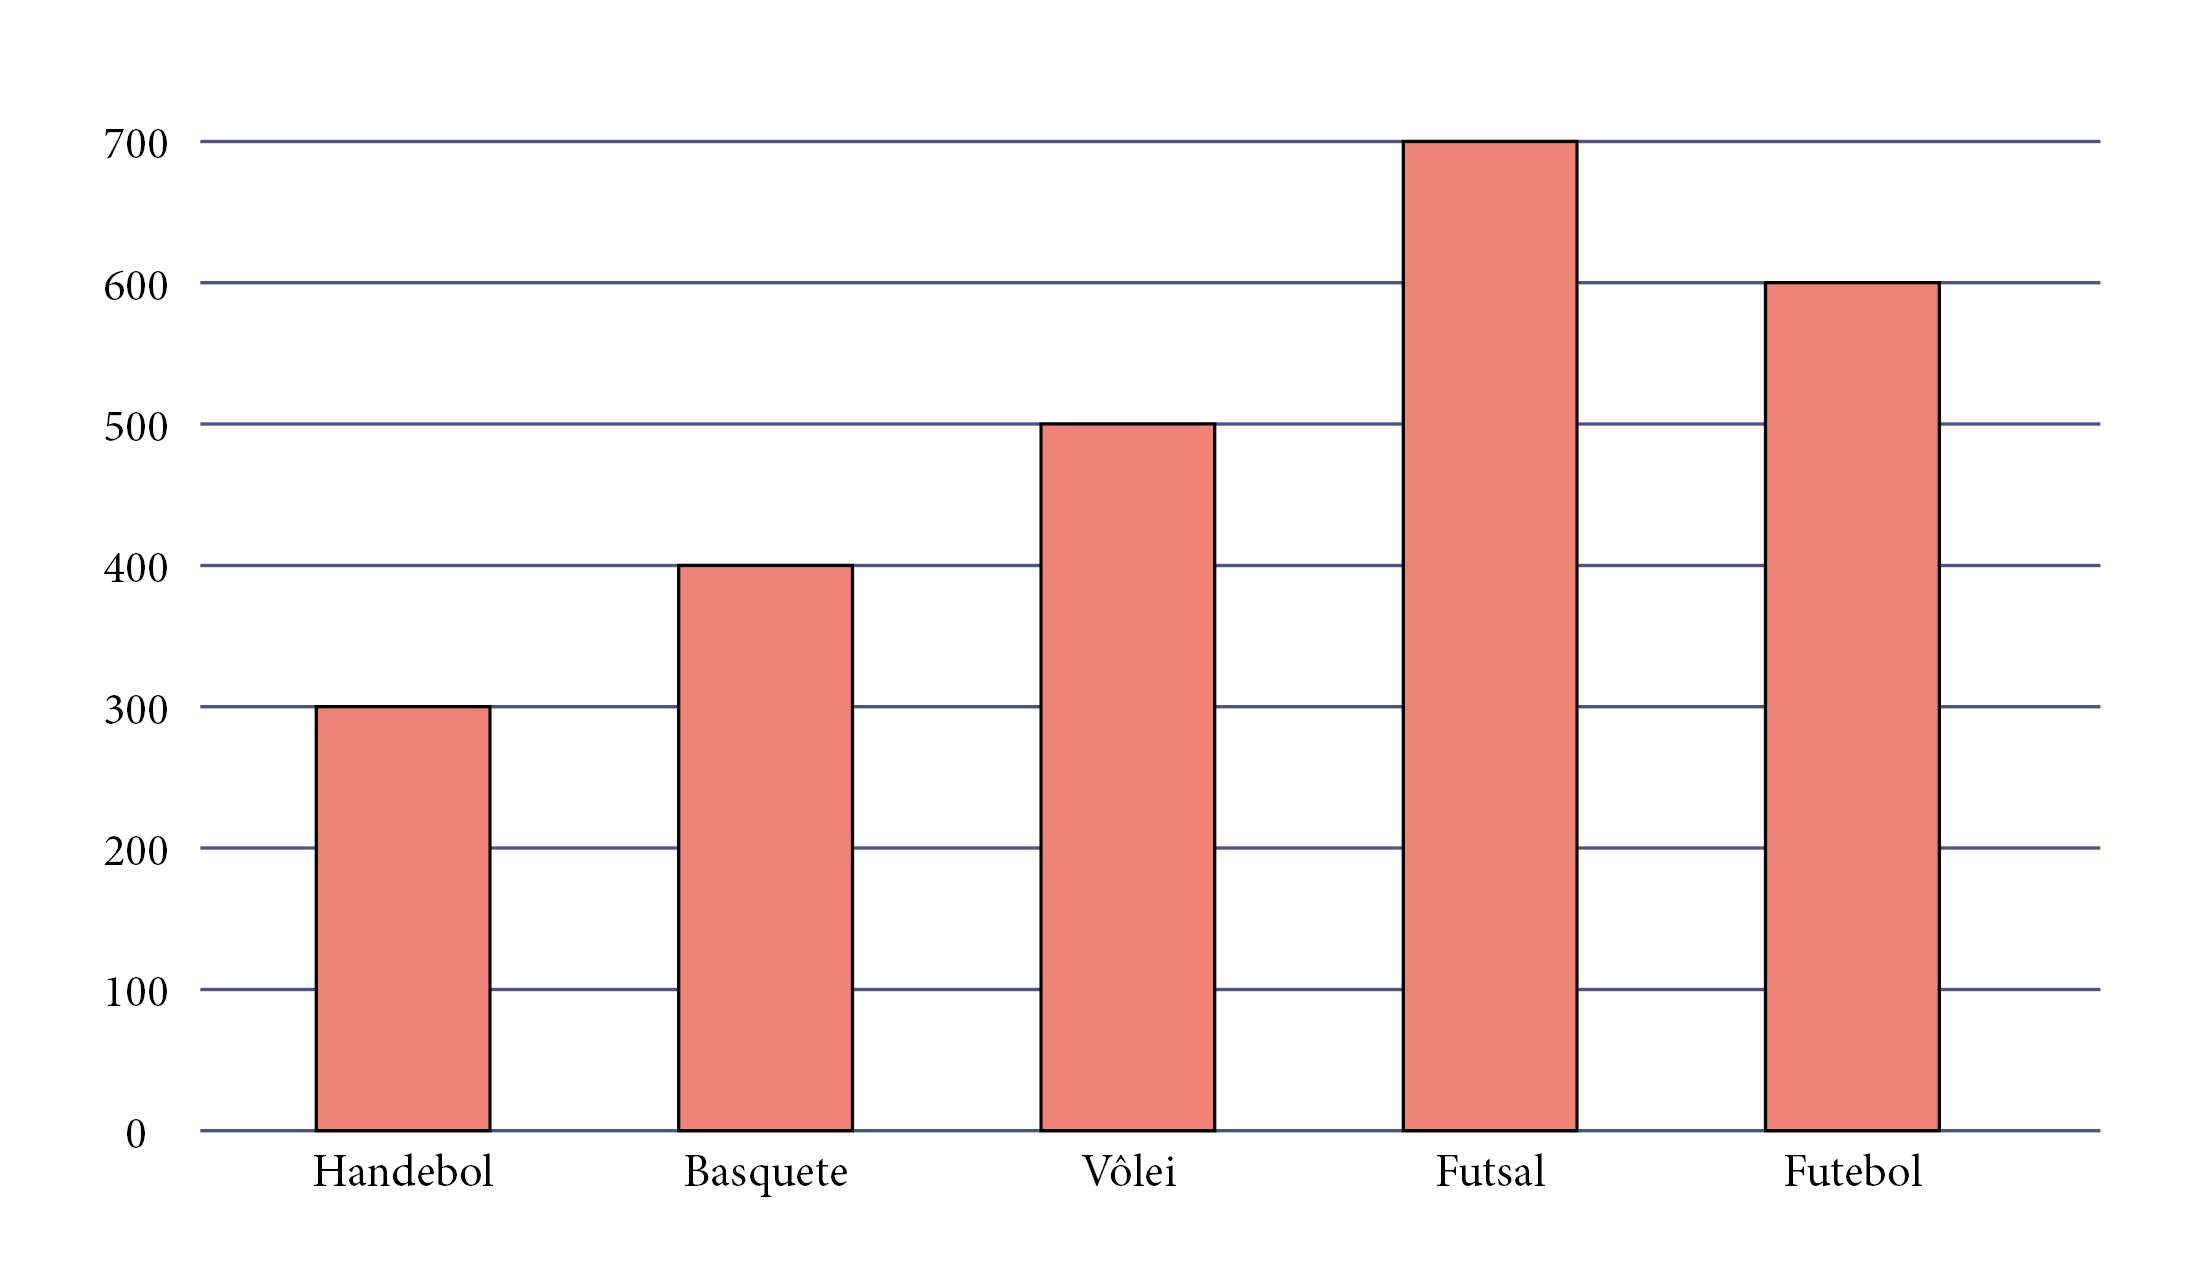
\includegraphics[width=.9\textwidth]{./media/image122.png}
\end{figure}

Indique o esporte que obteve o maior número de votos.

\begin{escolha}[itemsep=-5pt]
\item Basquete.

\item Futsal.

\item Handebol.

\item Vôlei.
\end{escolha}

\chapter[Simulado 2]{Simulado}
\markboth{Simulado 2}{}

\num{1}

A figura a seguir mostra o total de pontos obtidos por Artur, Bruna, César
e Dulce em um jogo. Quem fez mais pontos?

\begin{figure}[H]

\includegraphics[width=\textwidth]{./media/image124.png}
\end{figure}

\begin{escolha}[itemsep=-5pt]
\item Artur.

\item Bruna.

\item César.

\item Dulce.
\end{escolha}

\num{2} Veja o preço de alguns produtos de uma loja. Qual é o produto mais
barato?

\begin{figure}[H]
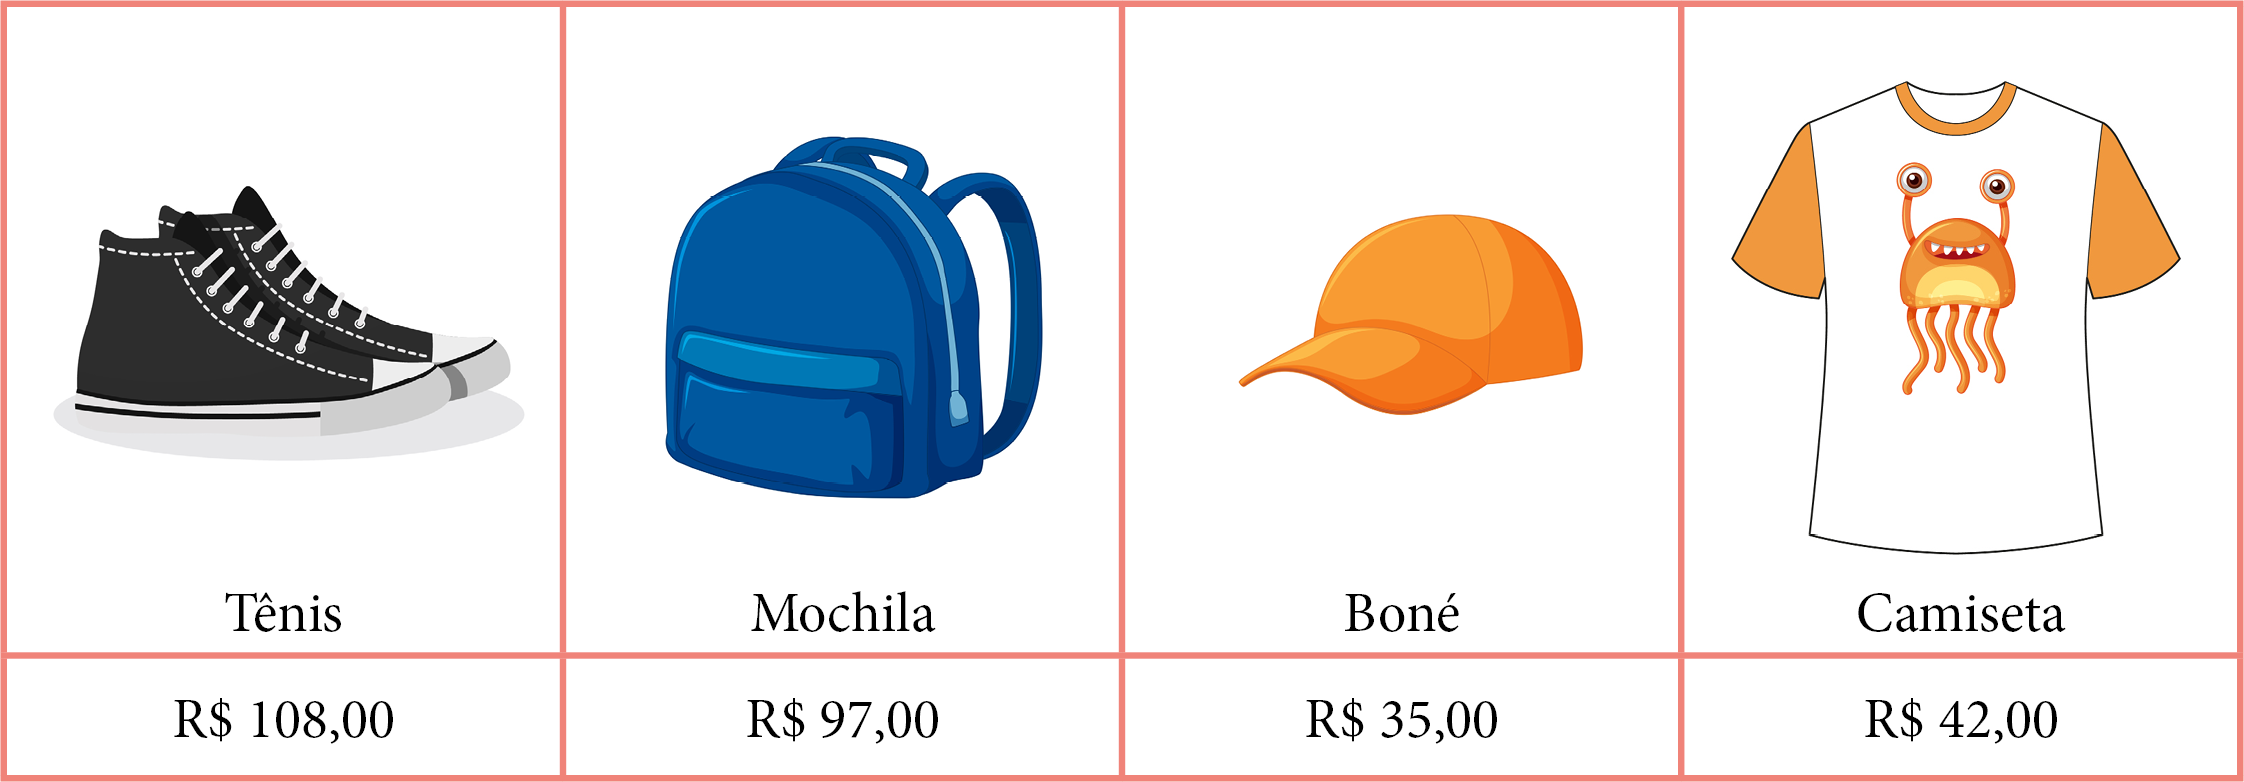
\includegraphics[width=\textwidth]{./media/image125.png}
\end{figure}

\begin{escolha}[itemsep=-5pt]
\item Boné.

\item Camiseta.

\item Mochila.

\item Tênis.
\end{escolha}

\num{3} Para abrir um determinado cofre, é necessário digitar três algarismos
desconhecidos. Analise as pistas e descubra a senha correta do cofre.

\begin{itemize}
\item
  O algarismo das centenas é maior que 1 e menor que 3.
\item
  O algarismo das dezenas é menor que 4 e maior que 2.
\item
  O algarismo das unidades é maior que 7 e menor que 9.
\end{itemize}

%\begin{figure}[H]
%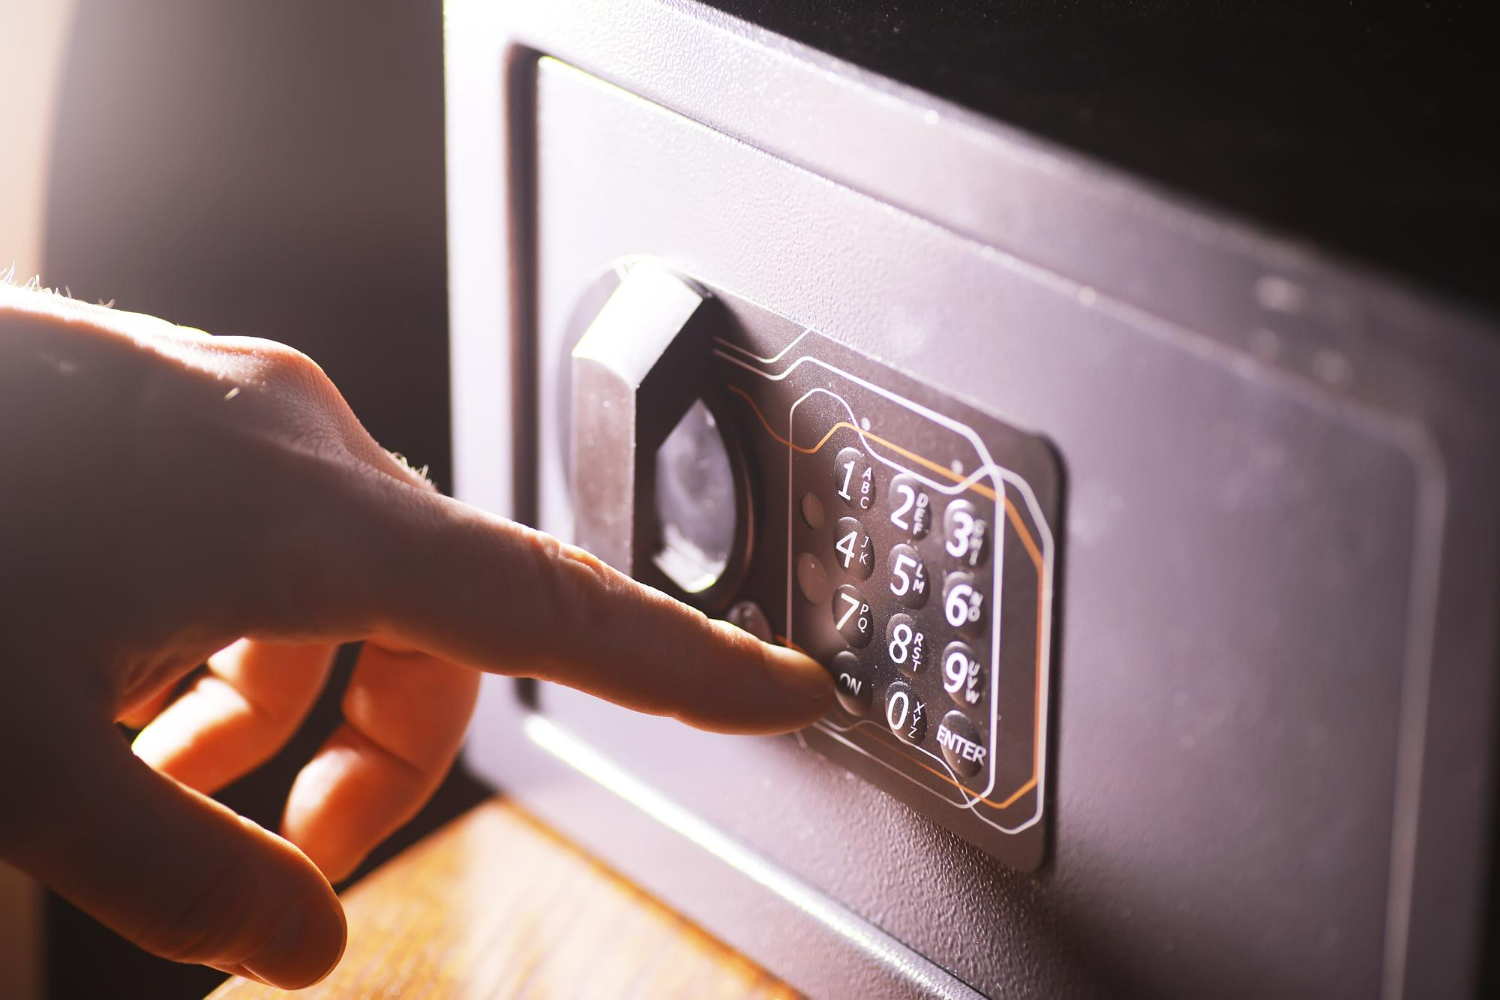
\includegraphics[width=\textwidth]{./media/image126.png}
%\end{figure}

\begin{escolha}[itemsep=-5pt]
\item 139

\item 238

\item 247

\item 327
\end{escolha}

\num{4} Gabriel tinha 18 pirulitos e deu 5 para seu primo. Com quantos
pirulitos Gabriel ficou?

\begin{escolha}[itemsep=-5pt]
\item 11

\item 12

\item 13

\item 14
\end{escolha}

\num{5} Indique qual das adições a seguir pode ter como resultado o número 132.

\begin{escolha}[itemsep=-5pt]
\item 31 + 31 + 31 + 31

\item 32 + 32 + 32 + 32

\item 33 + 33 + 33 + 33

\item 34 + 34 + 34 + 34
\end{escolha}

\num{6} Qual medida é obtida pelo instrumento da figura?

\begin{figure}[H]
\centering
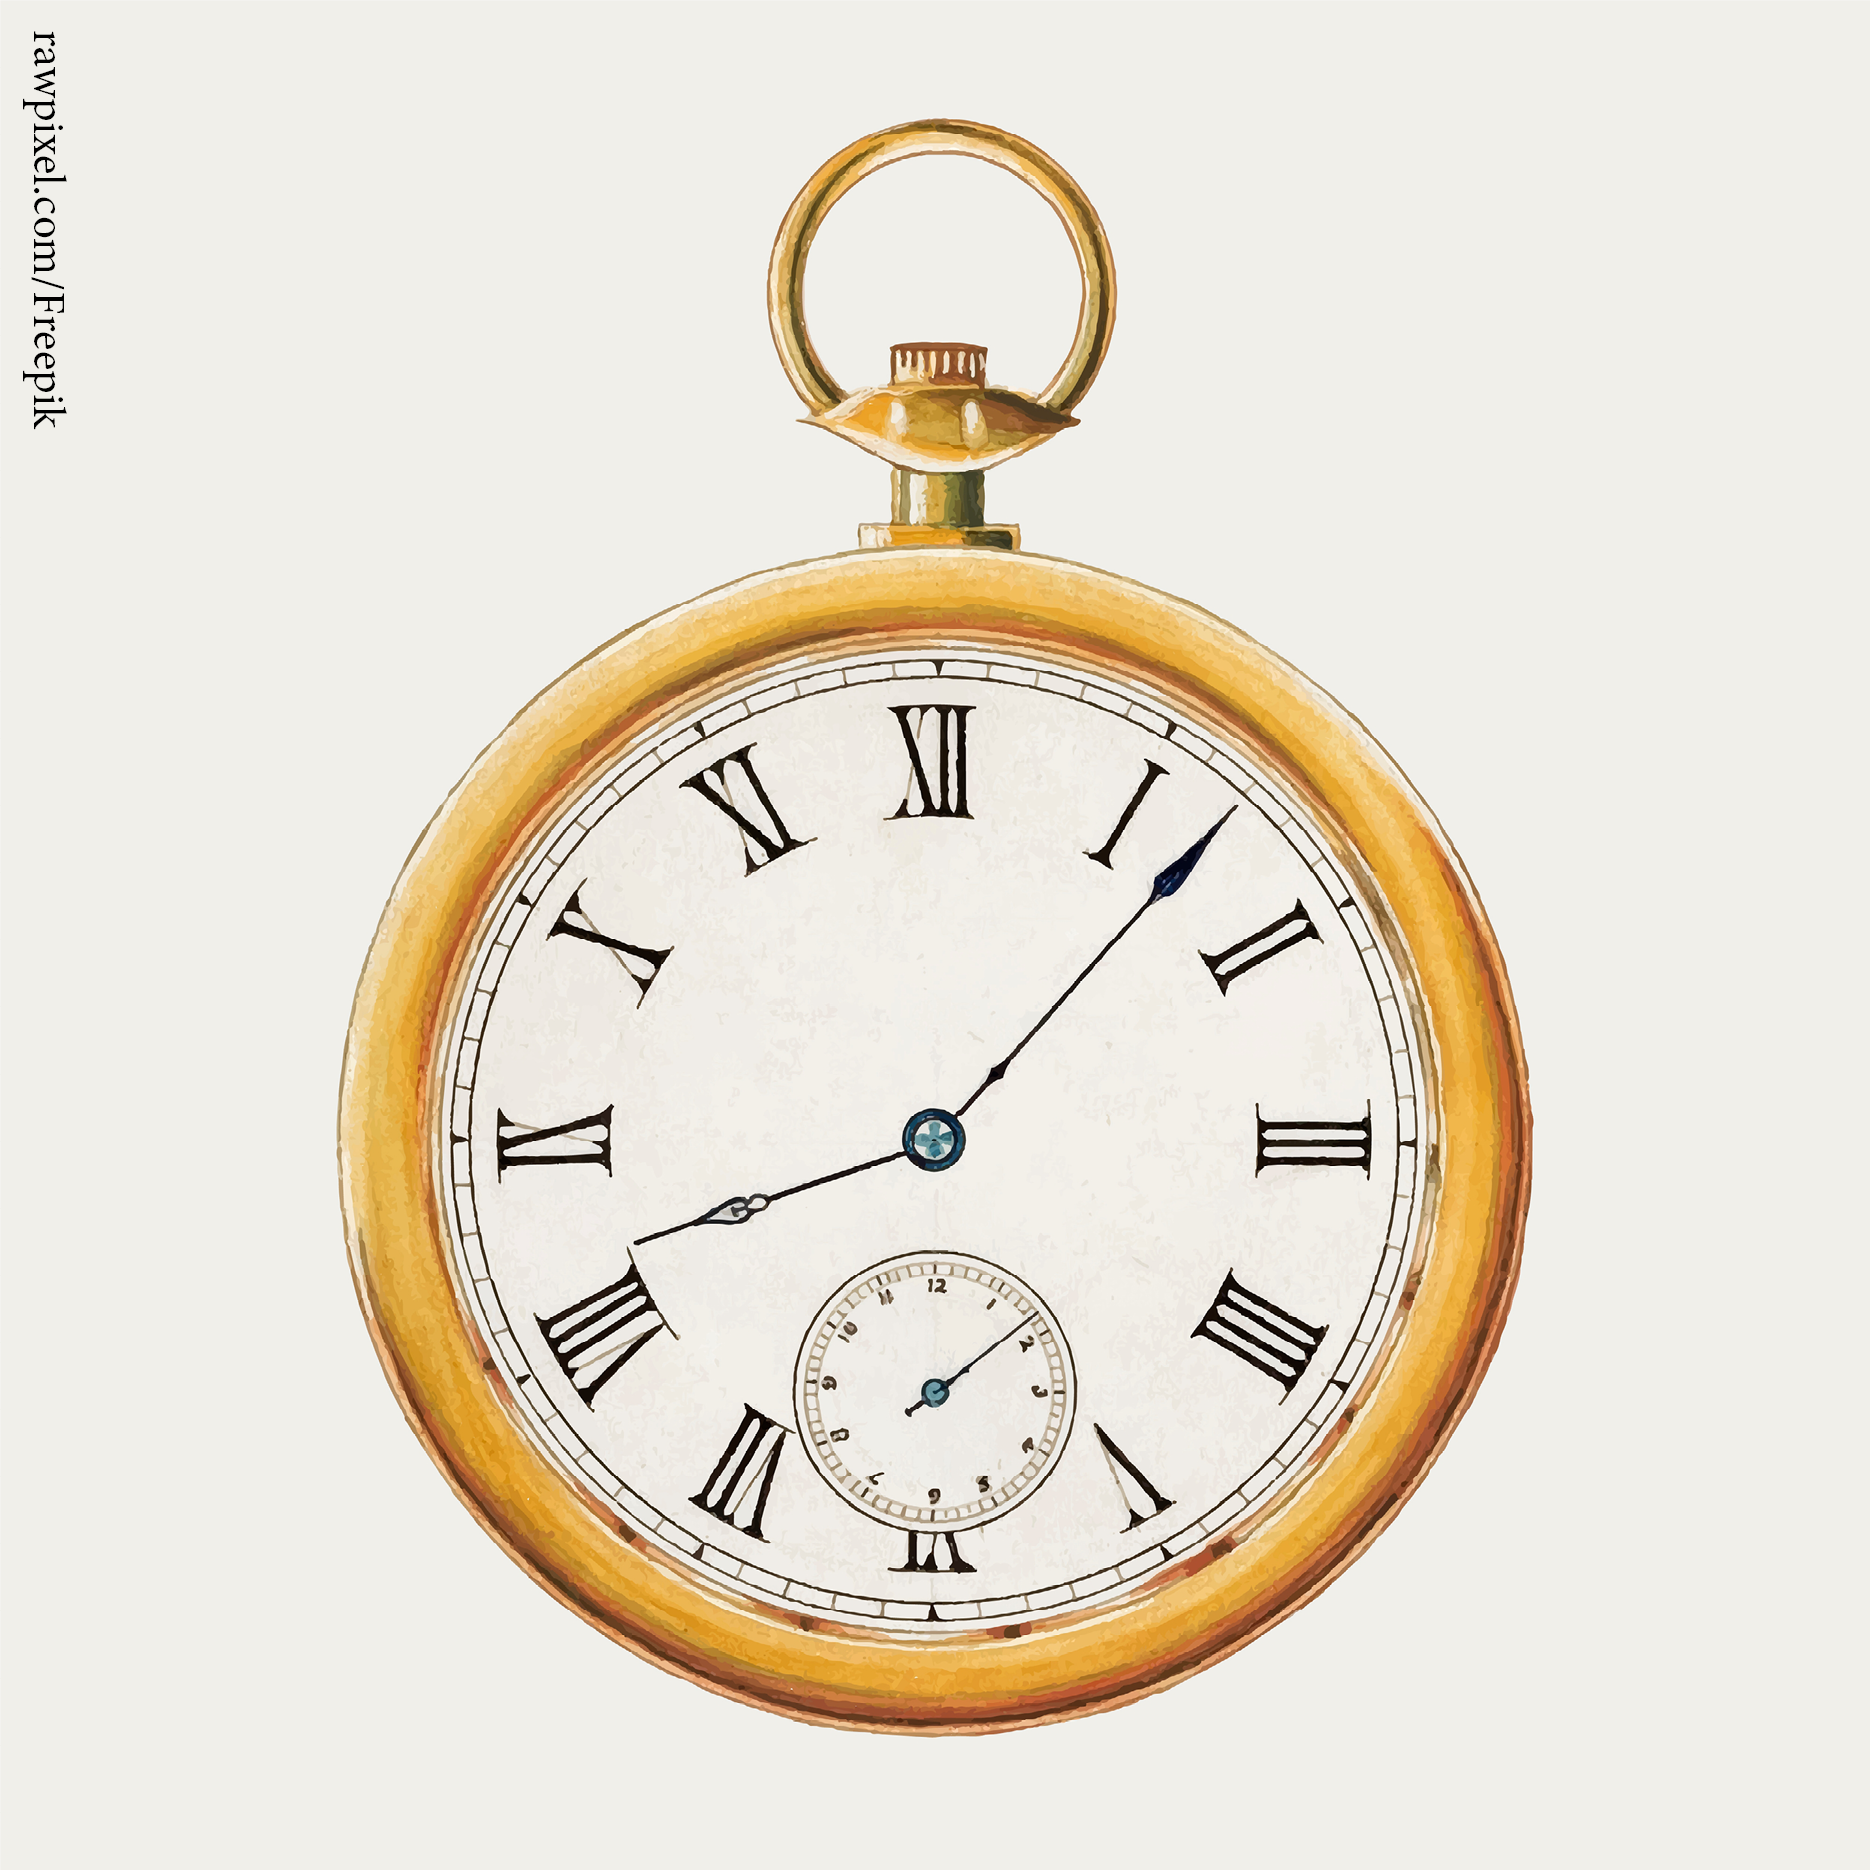
\includegraphics[width=.3\textwidth]{./media/image129.png}
\end{figure}

\begin{escolha}[itemsep=-5pt]
\item Capacidade.

\item Comprimento.

\item Massa.

\item Tempo.
\end{escolha}

\num{7} O professor de Educação Física precisa medir a distância de uma ponta a
outra da quadra da escola. Qual é o melhor instrumento para fazer essa
medição?

%\begin{figure}[H]
%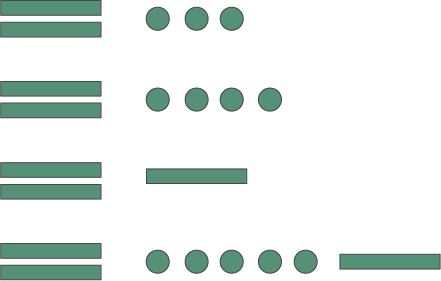
\includegraphics[width=\textwidth]{./media/image127.png}
%\end{figure}

\begin{figure}[H]
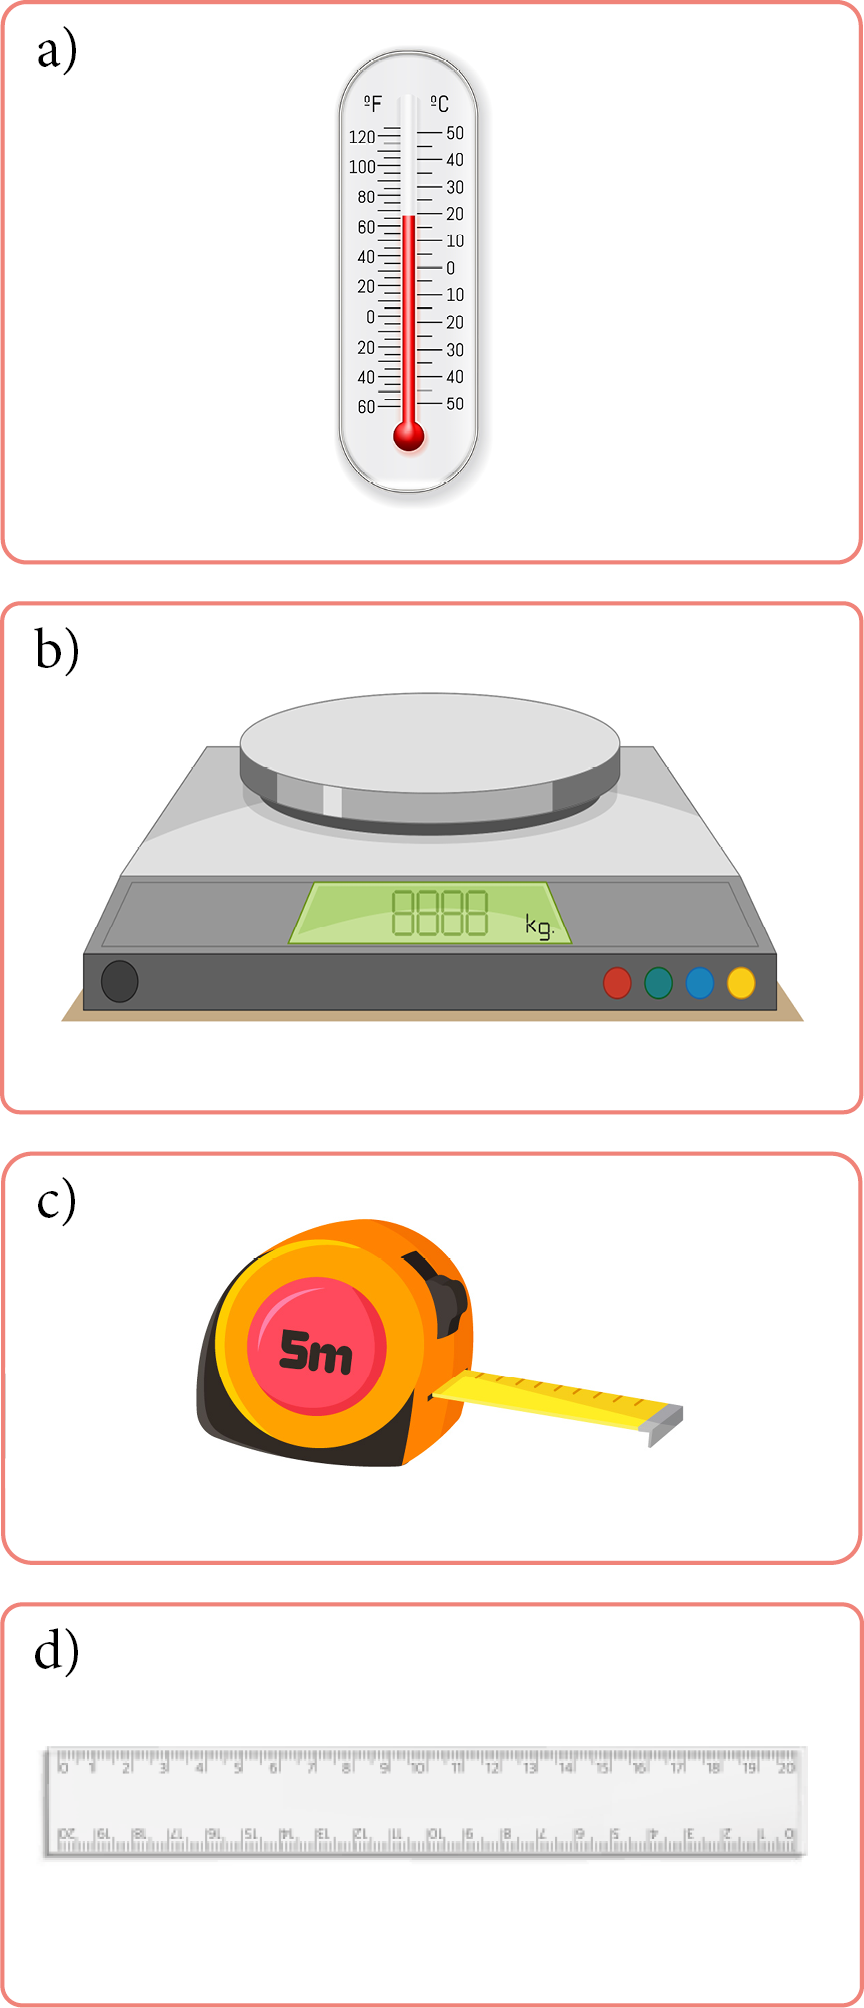
\includegraphics[width=.45\textwidth]{./media/image128.png}
\end{figure}


\num{8} Observe o calendário do mês de julho do ano de 2023. As férias escolares
de Lorena se iniciam no primeiro dia desse mês e ela vai passar três
semanas com sua tia, que mora no litoral. Quais dias do mês de julho
Lorena passará com a sua tia?

\begin{figure}[H]
\centering
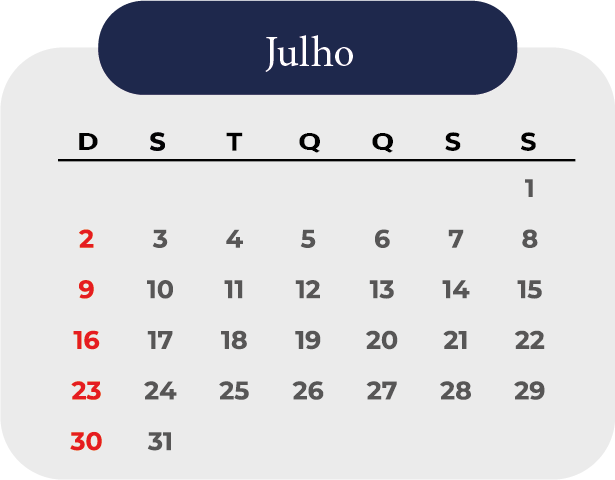
\includegraphics[width=.7\textwidth]{./media/image130.png}
\end{figure}

\begin{escolha}[itemsep=-5pt]
\item 2 a 22

\item 9 a 24

\item 16 a 29

\item 23 a 31
\end{escolha}

\num{9} Um avião decolou do aeroporto de Brasília às 08:00 e pousou em seu
destino, na cidade de São Paulo, às 09:45. Qual foi a duração da viagem?

\begin{escolha}[itemsep=-5pt]
\item 45 minutos.

\item 1 hora.

\item 1 hora e 45 minutos.

\item 2 horas e 15 minutos.
\end{escolha}

\num{10} Luciete foi ao sacolão e comprou 3 sacos de tomates. Cada saco vinha com
8 tomates. Quantos tomates ela comprou no total?

\begin{escolha}[itemsep=-5pt]
\item 8

\item 16

\item 24

\item 32
\end{escolha}

\num{11} Leonardo ganhou 100 reais de seu pai e comprou um brinquedo que custou
57 reais. Indique quanto sobrou para Leonardo depois de sua compra.

\begin{figure}[H]
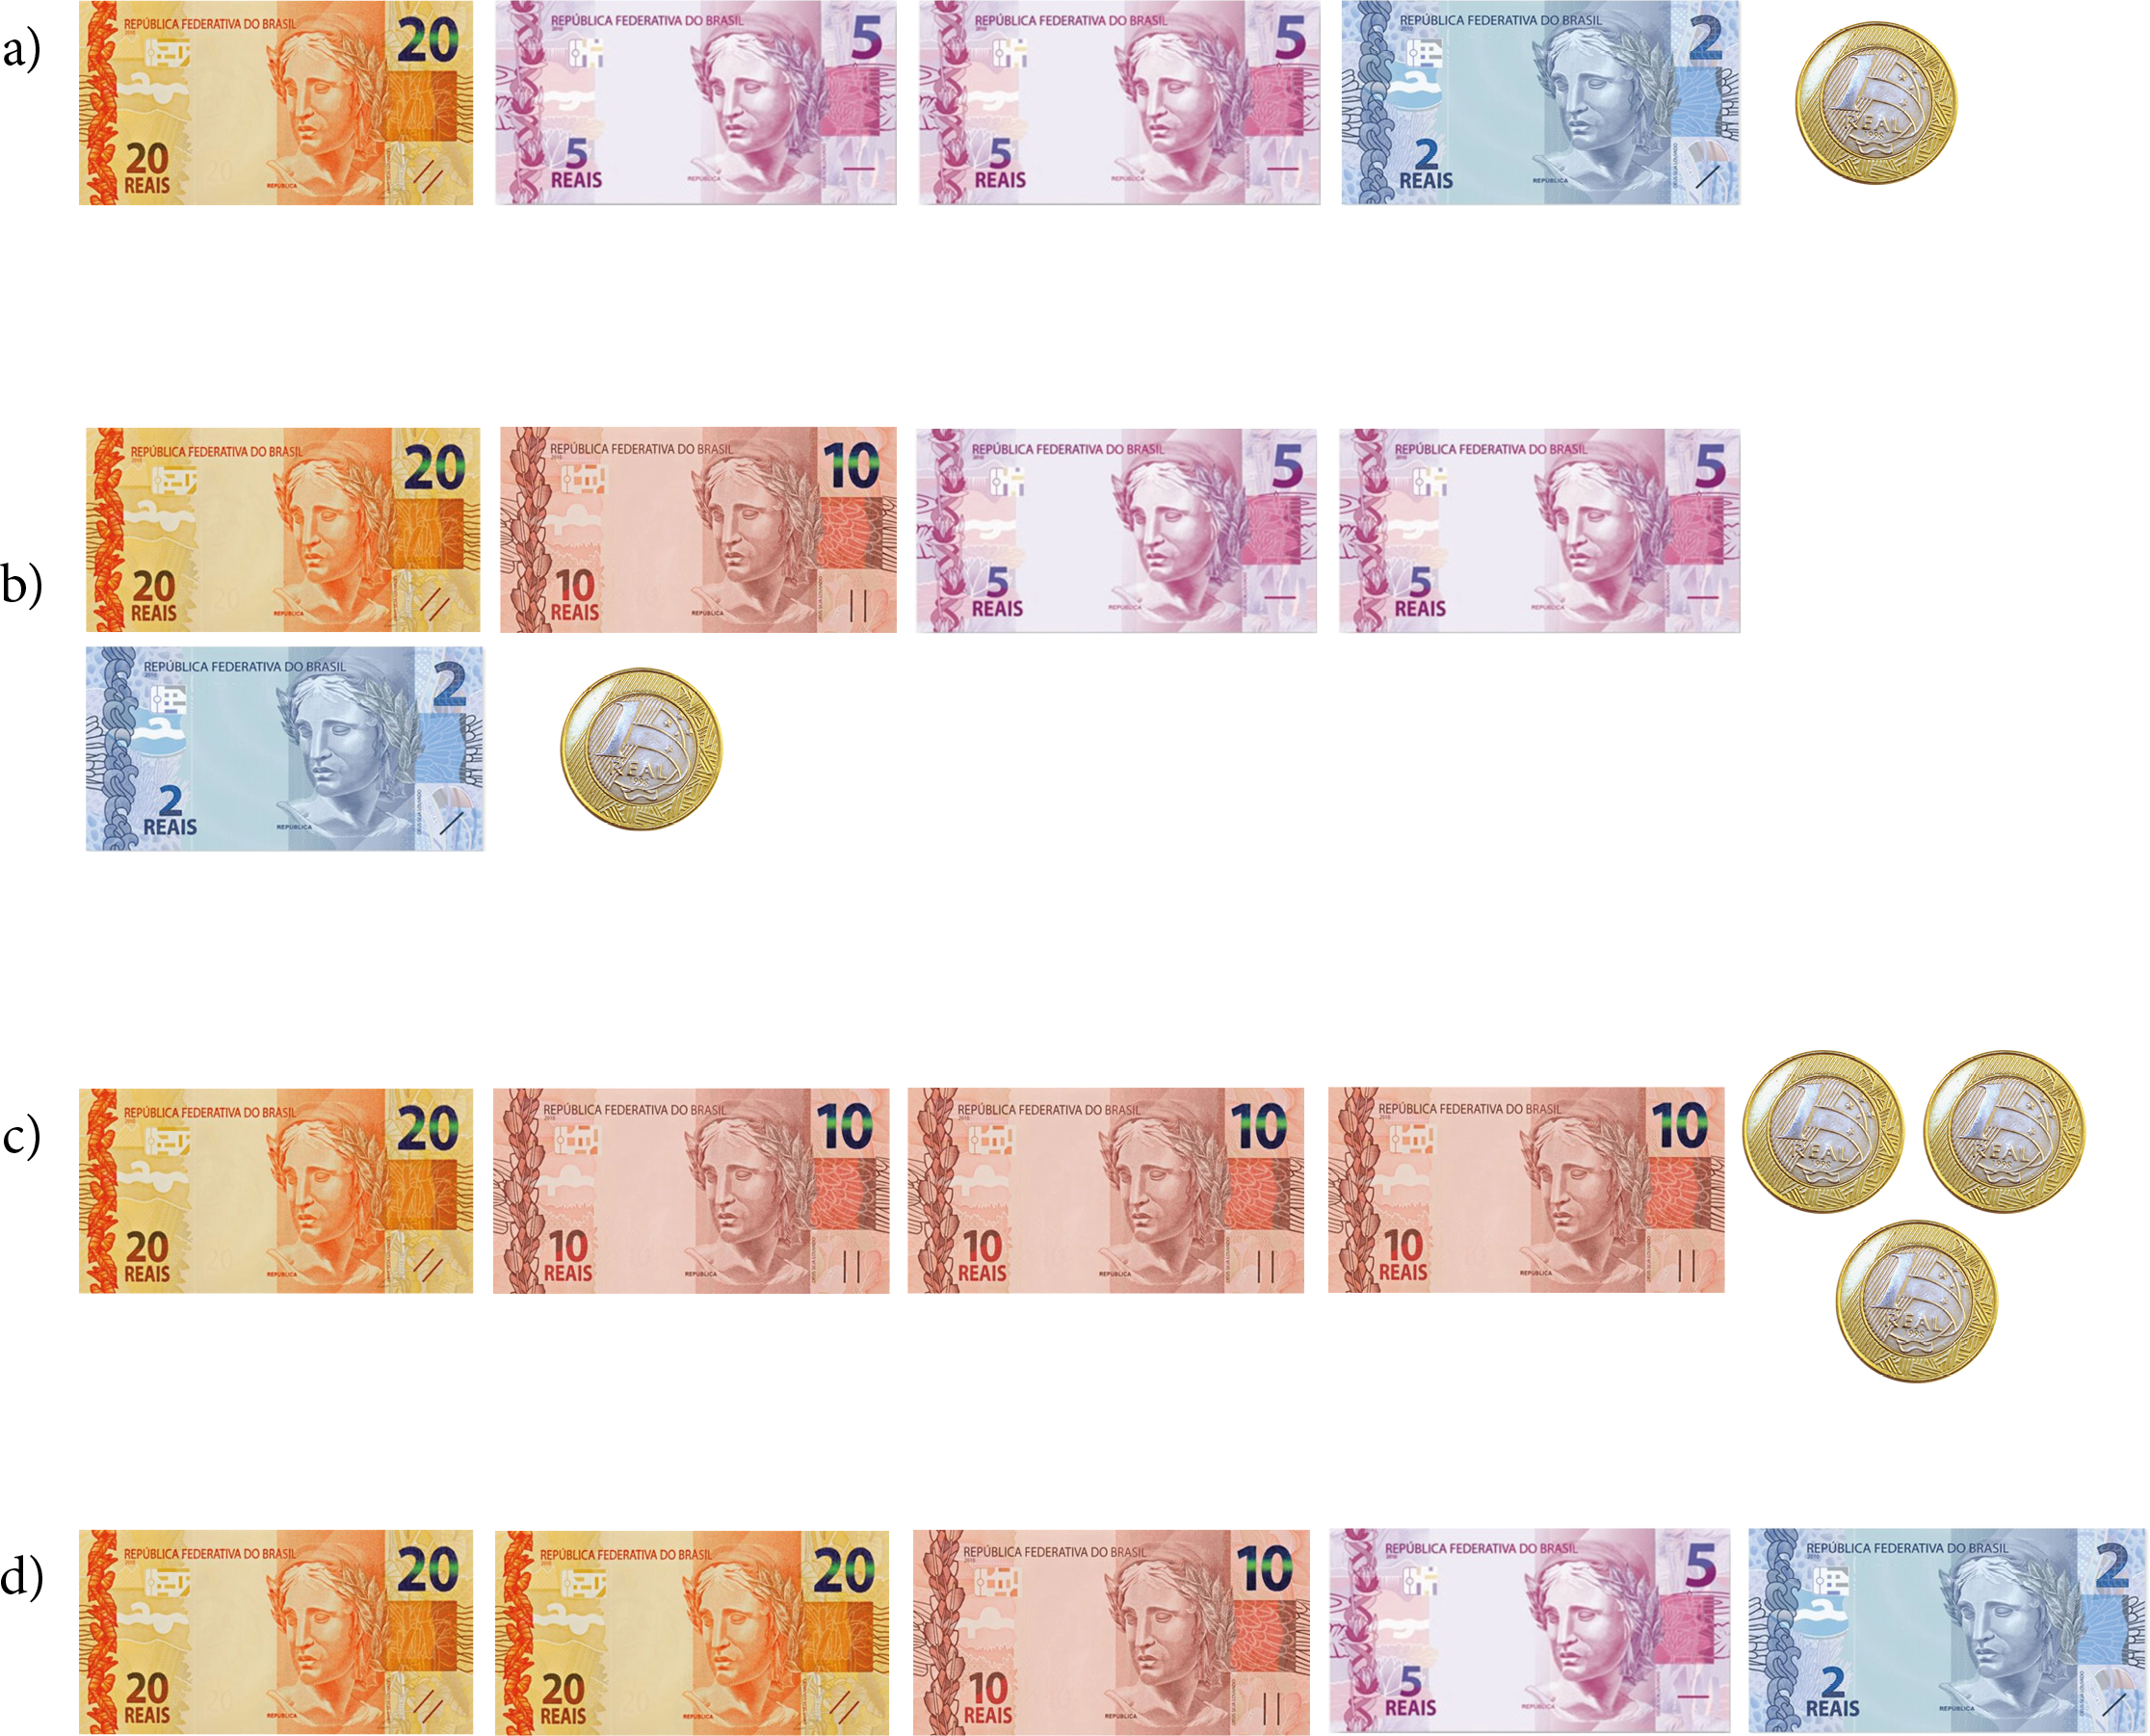
\includegraphics[width=\textwidth]{./media/image131.png}
\end{figure}

\num{12} Marcelo ganhou 20 reais de seu pai e deseja comprar uma bola. Ao chegar
à loja de brinquedos, ele percebeu que precisaria do dobro desse valor
para conseguir comprá-la. Qual o valor dessa bola?

\begin{escolha}[itemsep=-5pt]
\item R\$ 10,00

\item R\$ 20,00

\item R\$ 30,00

\item R\$ 40,00
\end{escolha}

\num{13} Isadora tem um saquinho com 29 gomas vermelhas e 6 pretas. Se ela tirar
uma goma do saquinho, sem olhar dentro dele, o que pode acontecer?

\begin{figure}[H]
\centering
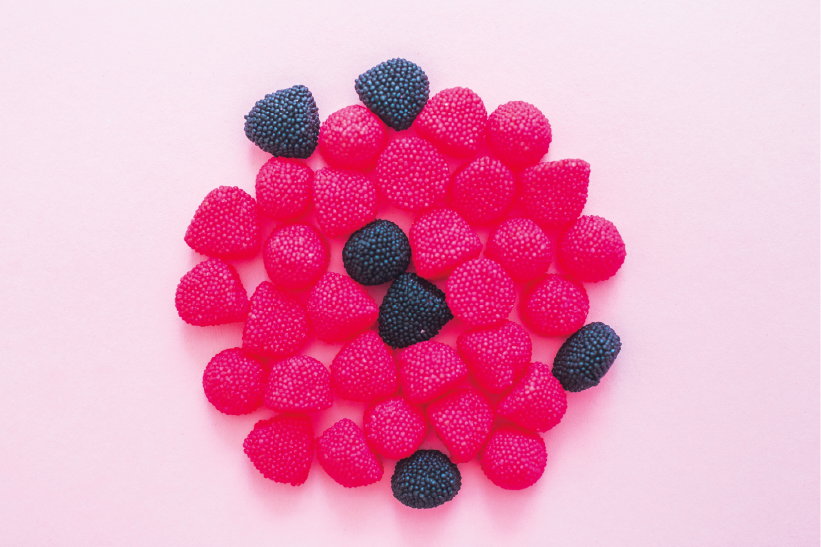
\includegraphics[width=.6\textwidth]{./media/image132.png}
\end{figure}

\begin{escolha}[itemsep=-5pt]
\item É muito provável que saia uma goma vermelha.

\item É muito provável que saia uma goma preta.

\item É pouco provável que saia uma goma vermelha.

\item É impossível que saia uma goma preta.
\end{escolha}


\num{14} Sofia explorou o quintal de sua casa e anotou em uma tabela a quantidade
de animaizinhos que encontrou. Observe a tabela.

\begin{figure}[H]
\centering
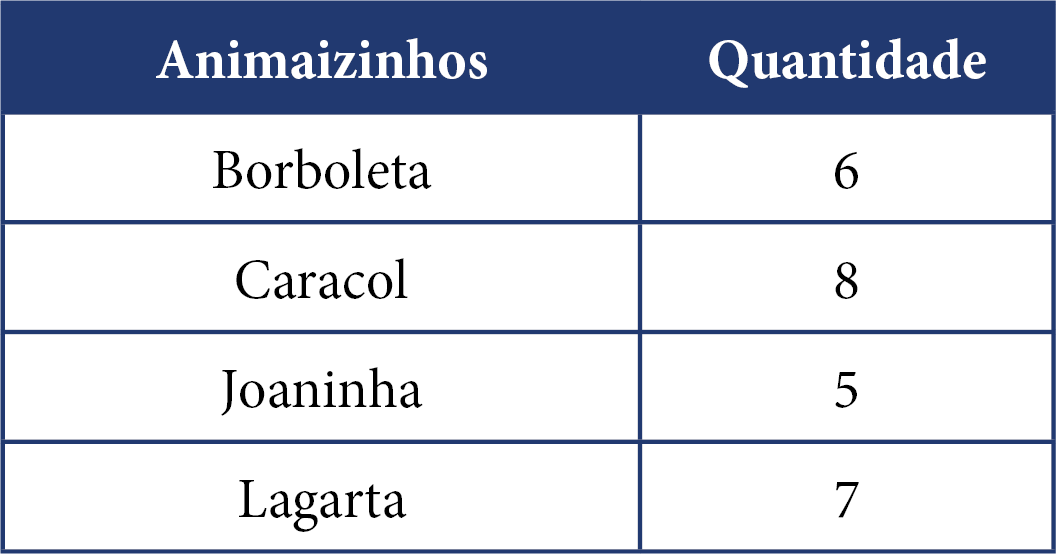
\includegraphics[width=.7\textwidth]{./media/image135.png}
\end{figure}

Quantas joaninhas e borboletas havia ao todo?

\begin{escolha}[itemsep=-5pt]
\item 11

\item 13

\item 14

\item 15
\end{escolha}

\num{15} A professora do 2º ano fez uma pesquisa com os alunos de suas duas
turmas (da manhã e da tarde) sobre as cores de que eles mais gostavam.
Analise o gráfico e indique a afirmativa verdadeira.

\begin{figure}[H]

\includegraphics[width=\textwidth]{./media/image136.png}
\end{figure}

\begin{escolha}[itemsep=-5pt]
\item Amarelo é a cor de que os alunos mais gostam.

\item A cor azul teve 25 votos.

\item Verde foi a cor menos votada.

\item Vermelho teve mais de 30 votos.
\end{escolha}

\chapter[Simulado 3]{Simulado}
\markboth{Simulado 3}{}

\num{1} Observe o número que aparece no visor da balança. O que esse número
representa?

\begin{figure}[H]
\centering
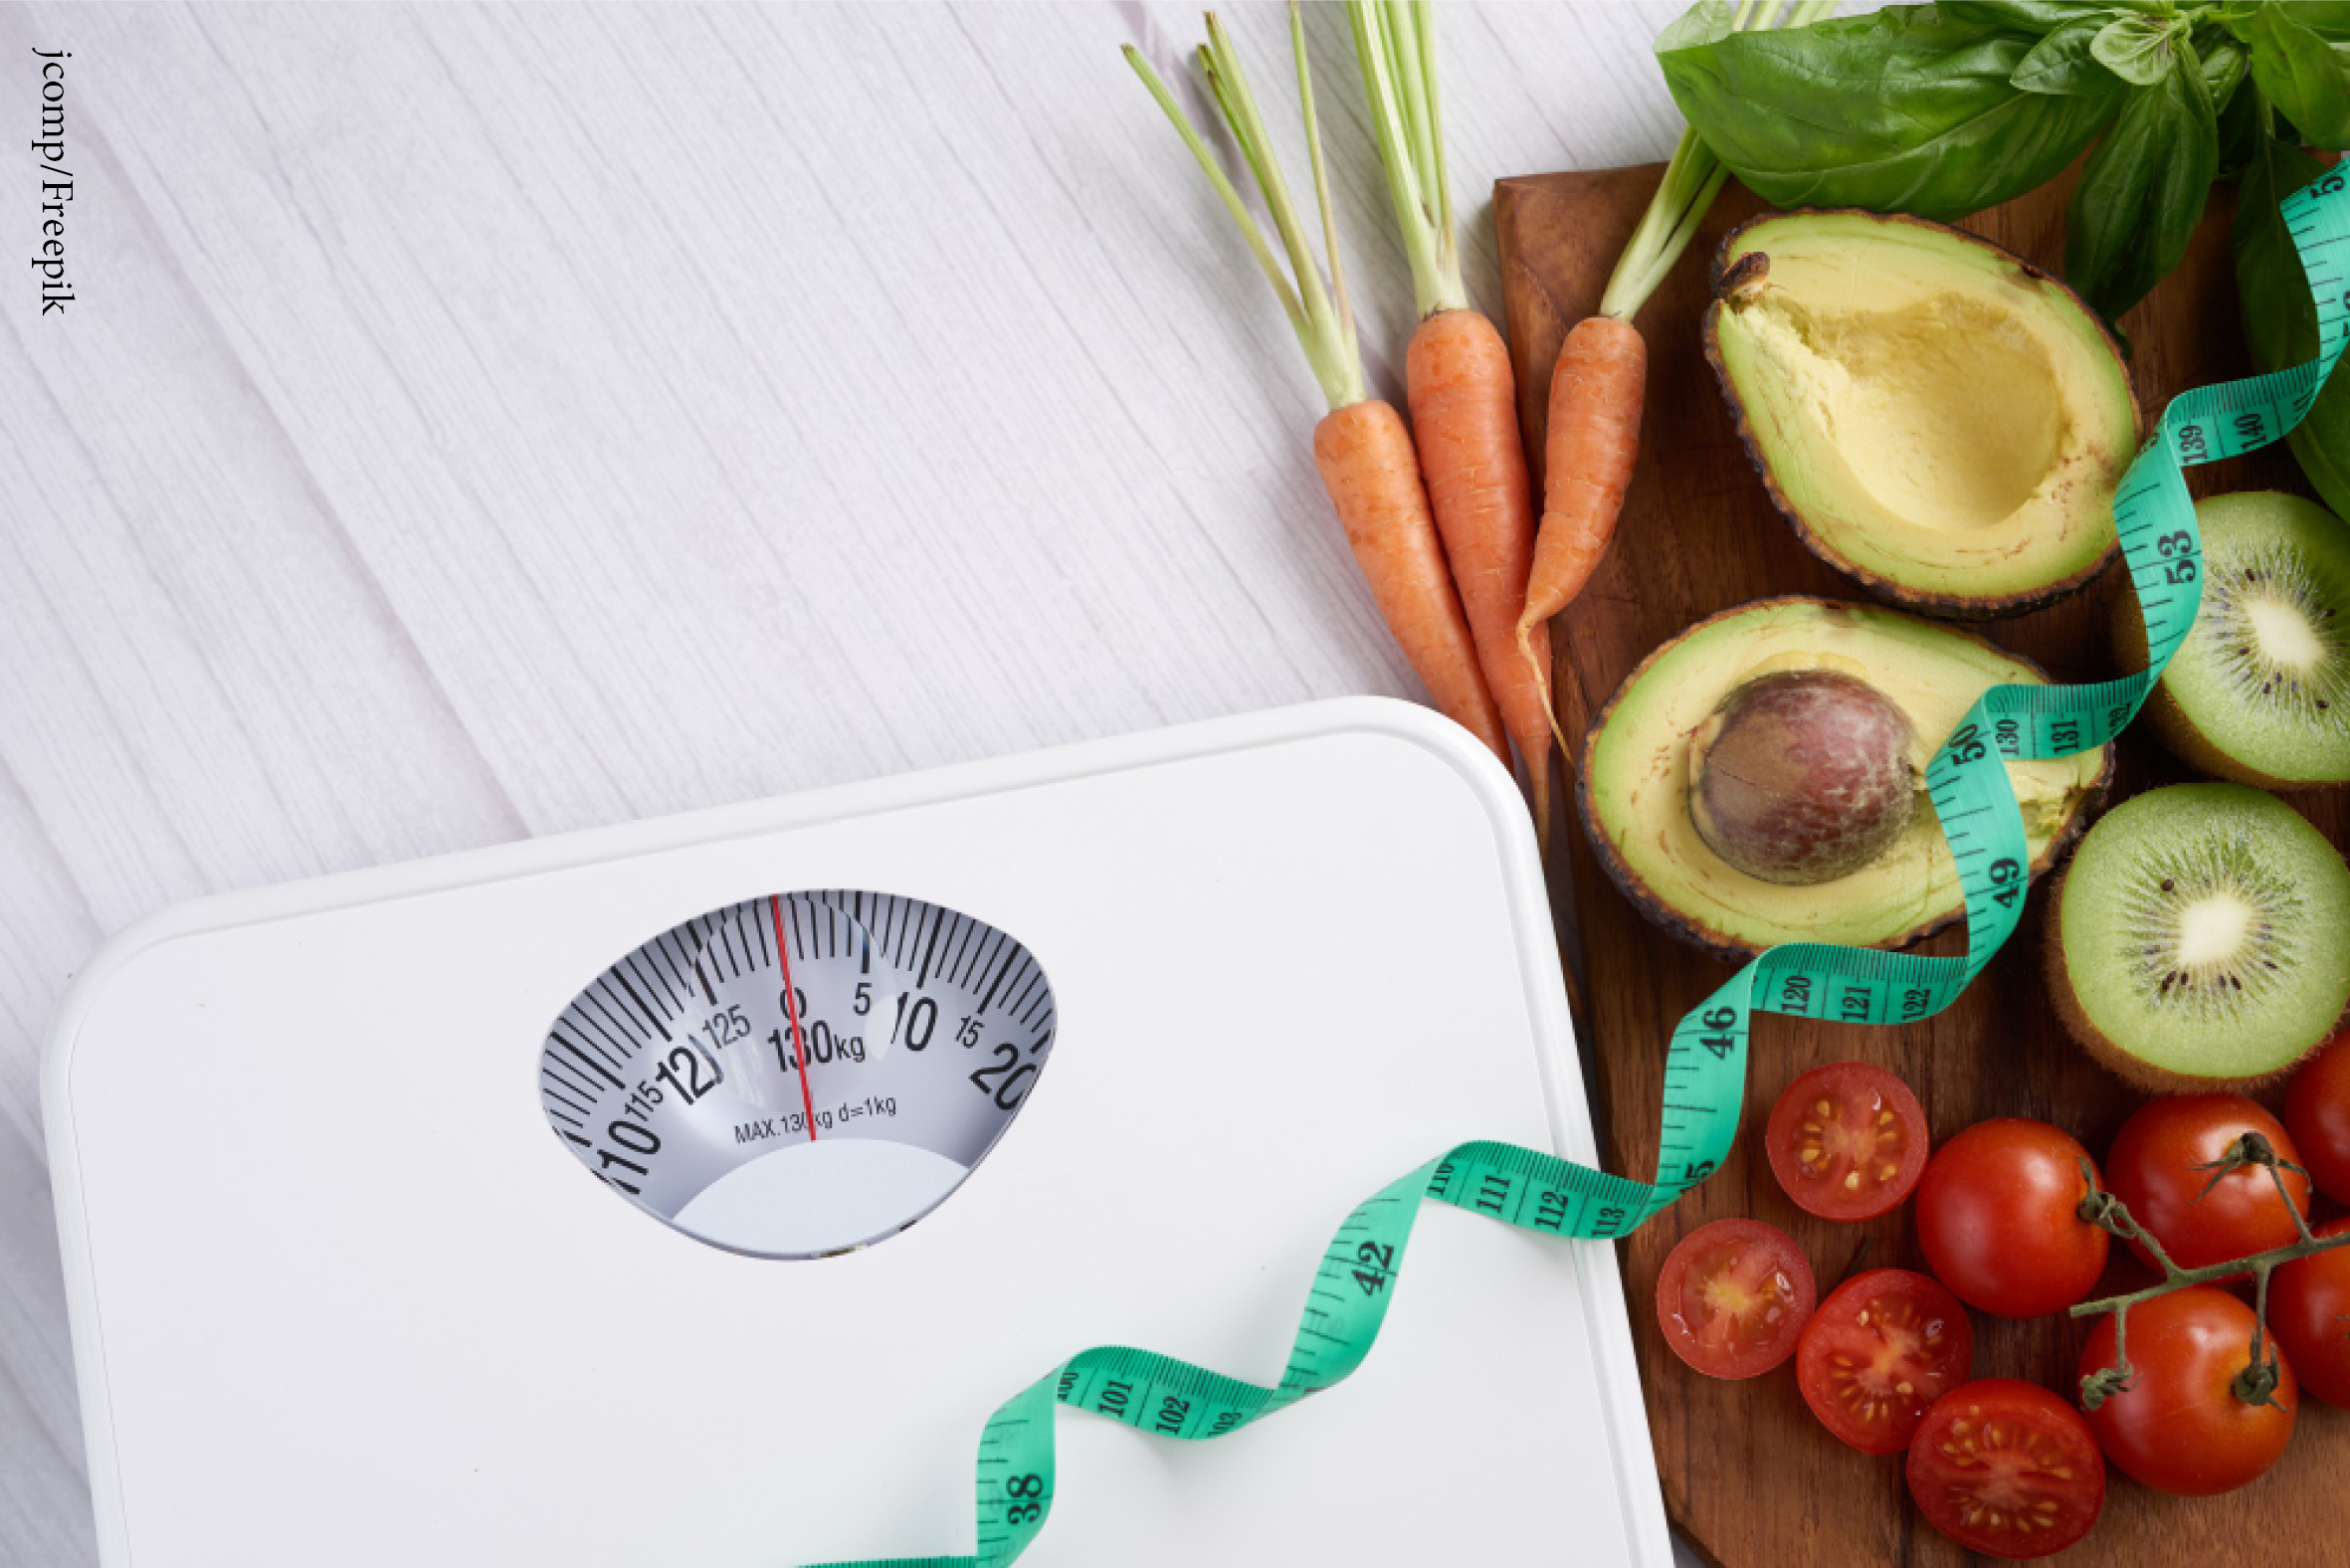
\includegraphics[width=.6\textwidth]{./media/image137.png}
\end{figure}

\begin{escolha}[itemsep=-5pt]
\item Código de identificação

\item Medida

\item Ordem

\item Quantidade
\end{escolha}


\num{2} Em uma corrida os(as) atletas utilizam números de identificação em suas
camisas para auxiliar no reconhecimento durante a prova. Sabendo disso,
indique o número do(a) atleta que está na primeira posição da corrida
mostrada a seguir.

\begin{figure}[H]

\includegraphics[width=\textwidth]{./media/image138.png}
\end{figure}

\begin{escolha}[itemsep=-5pt]
\item 07

\item 12

\item 31

\item 72
\end{escolha}

\num{3} Indique a única forma correta de compor o número 300.

\begin{escolha}[itemsep=-5pt]
\item 150 + 190 - 30

\item 160 + 200 - 40

\item 170 -- 30 + 150

\item 180 -- 70 + 190
\end{escolha}

\num{4} Ricardo convidou 48 amigos para sua festa de aniversário, porém, 9 não
puderam ir. Quantos amigos foram à festa?

\begin{escolha}[itemsep=-5pt]
\item 38

\item 39

\item 40

\item 41
\end{escolha}

\num{5} Observe a altura de cada animal e marque a alternativa que apresenta a
ordem correta do menor para o maior.

\begin{figure}[H]
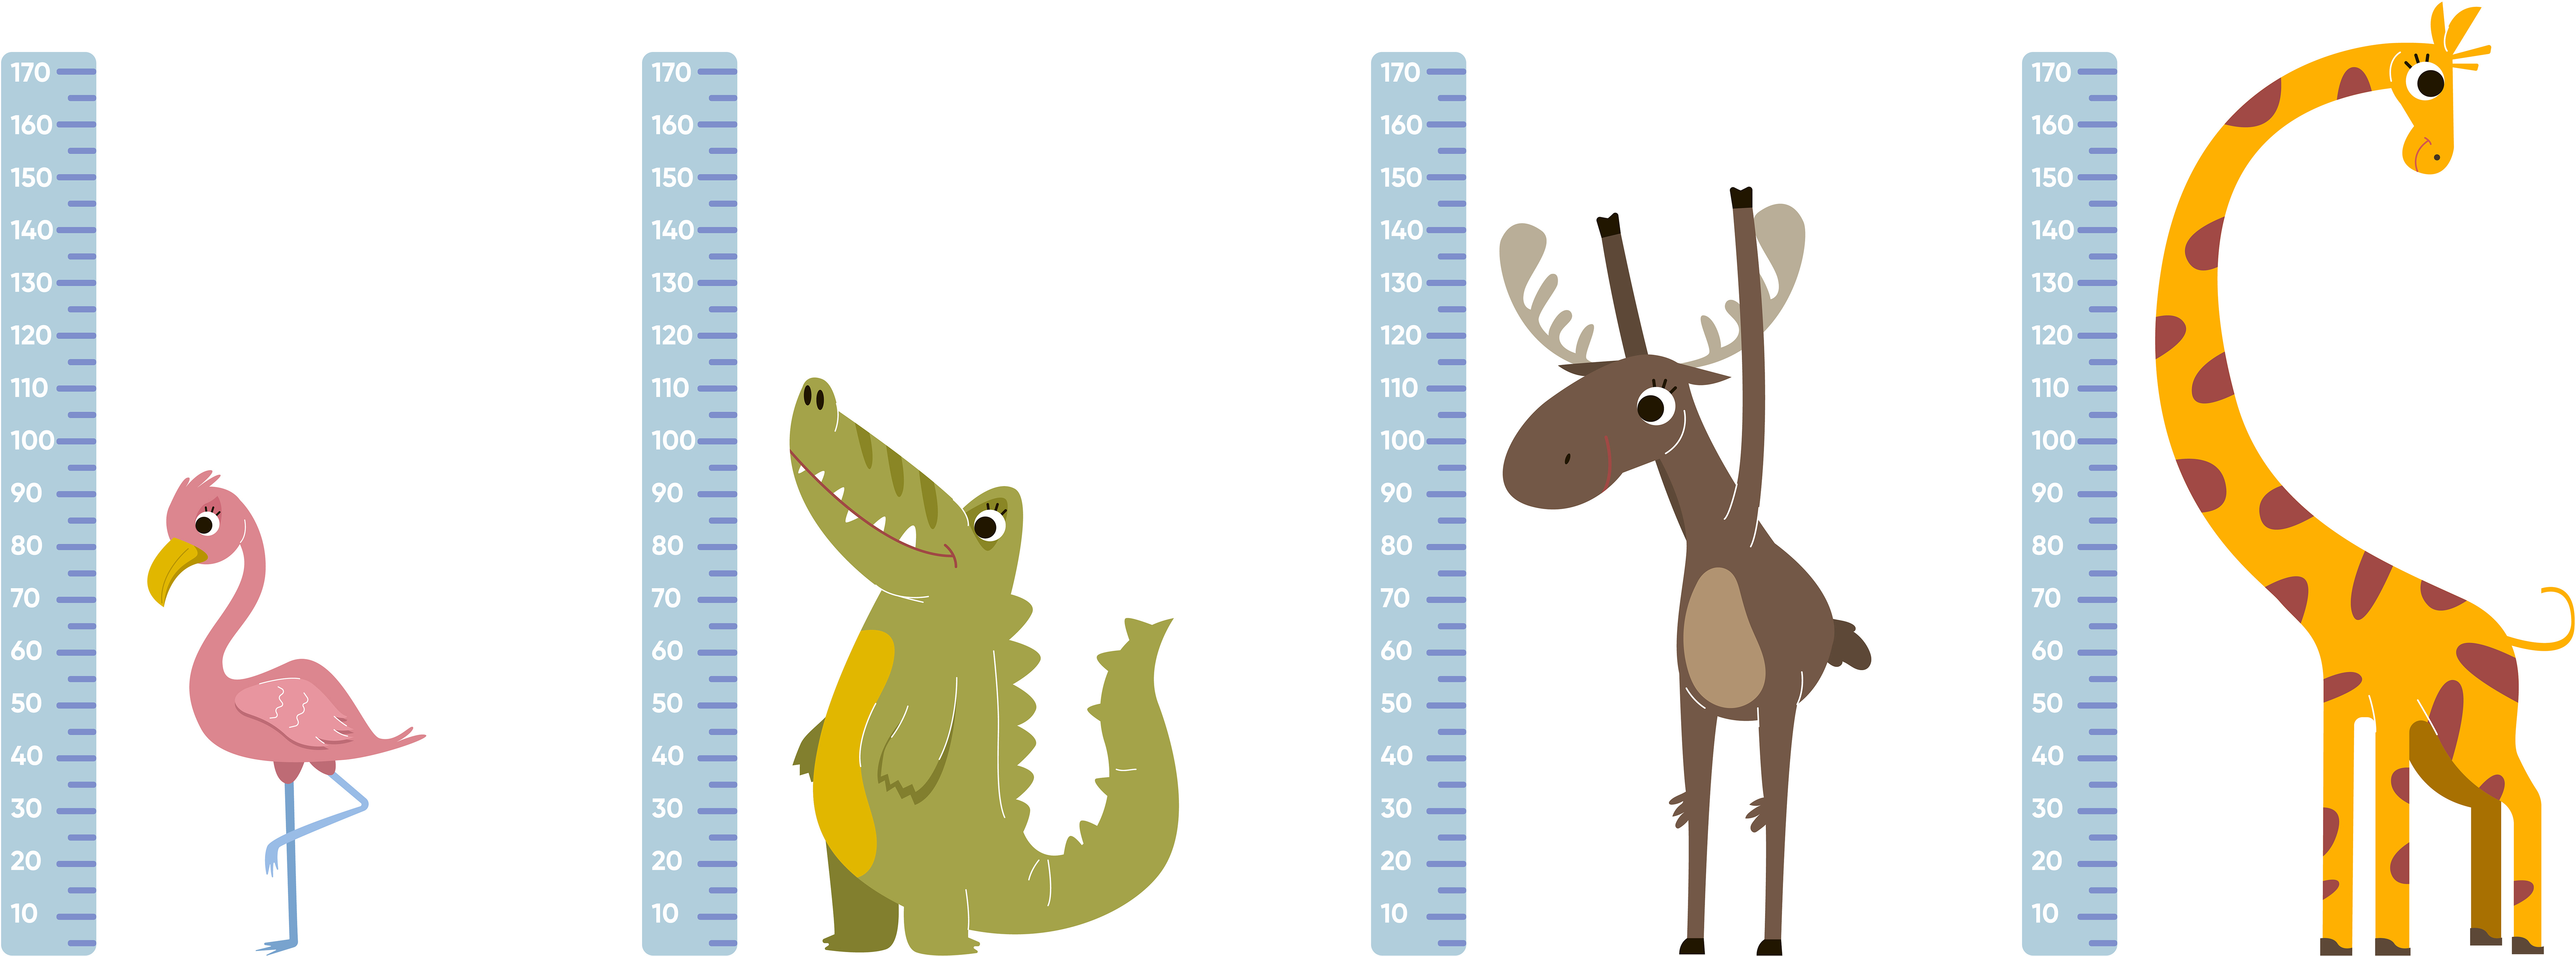
\includegraphics[width=\textwidth]{./media/image139.png}
\end{figure}

\begin{escolha}[itemsep=-5pt]
\item Alce -- Flamingo -- Girafa -- Jacaré.

\item Flamingo -- Jacaré -- Alce -- Girafa.

\item Girafa -- Alce -- Jacaré -- Flamingo.

\item Jacaré -- Flamingo -- Alce -- Girafa.
\end{escolha}

\num{6} Analise a figura e veja o que acontece quando é adicionado um copo de
água na jarra vazia. Depois indique como a jarra ficaria se, em vez de
adicionar um copo, fossem adicionados 5 copos de água.

\begin{figure}[H]
\centering
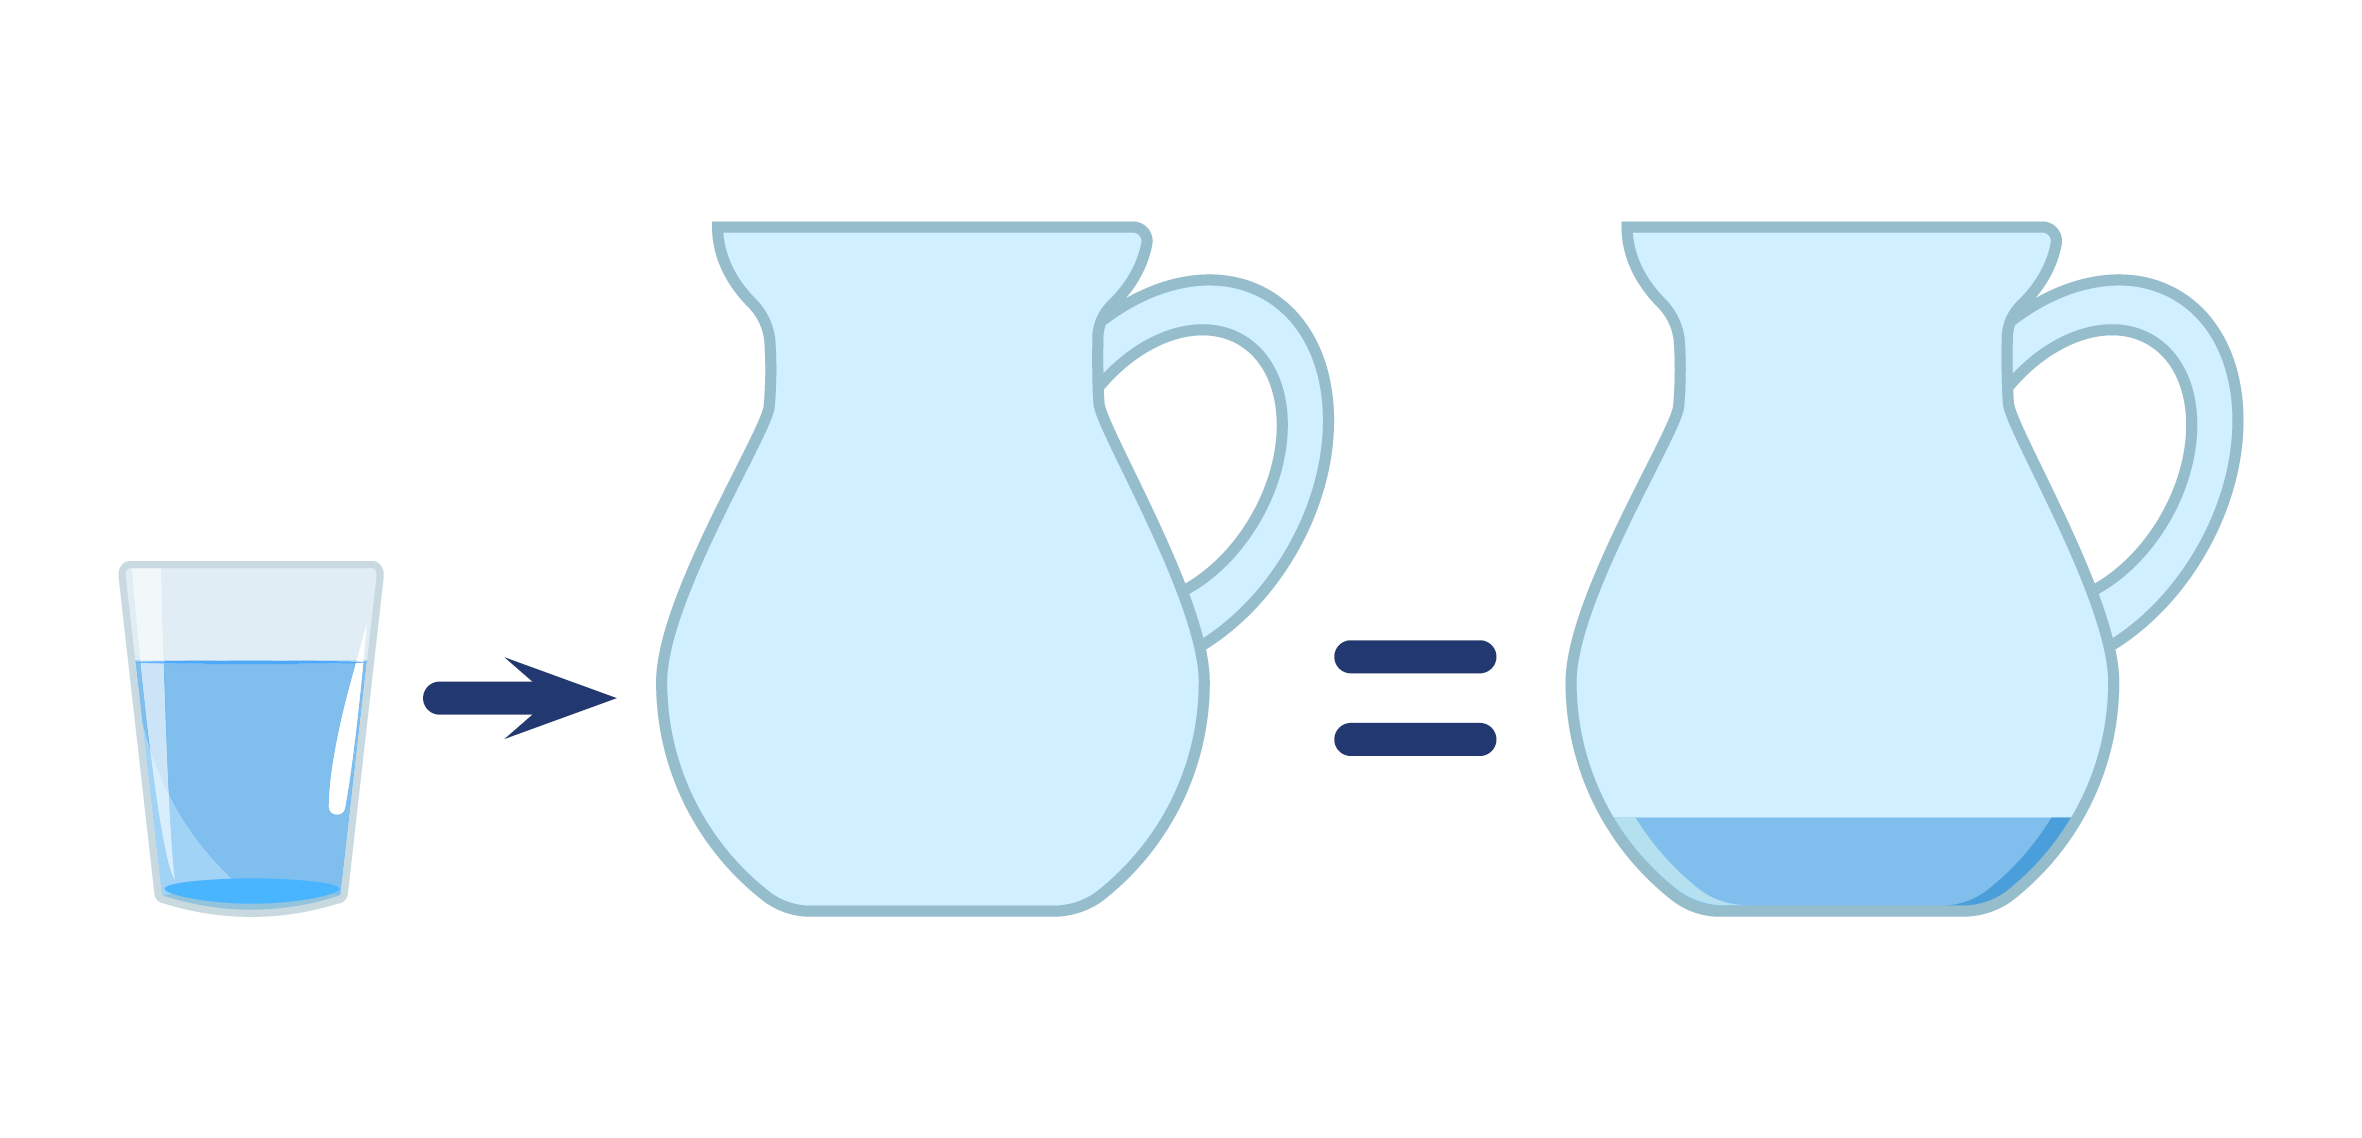
\includegraphics[width=\textwidth]{./media/image140.png}
\end{figure}

\begin{figure}[H]
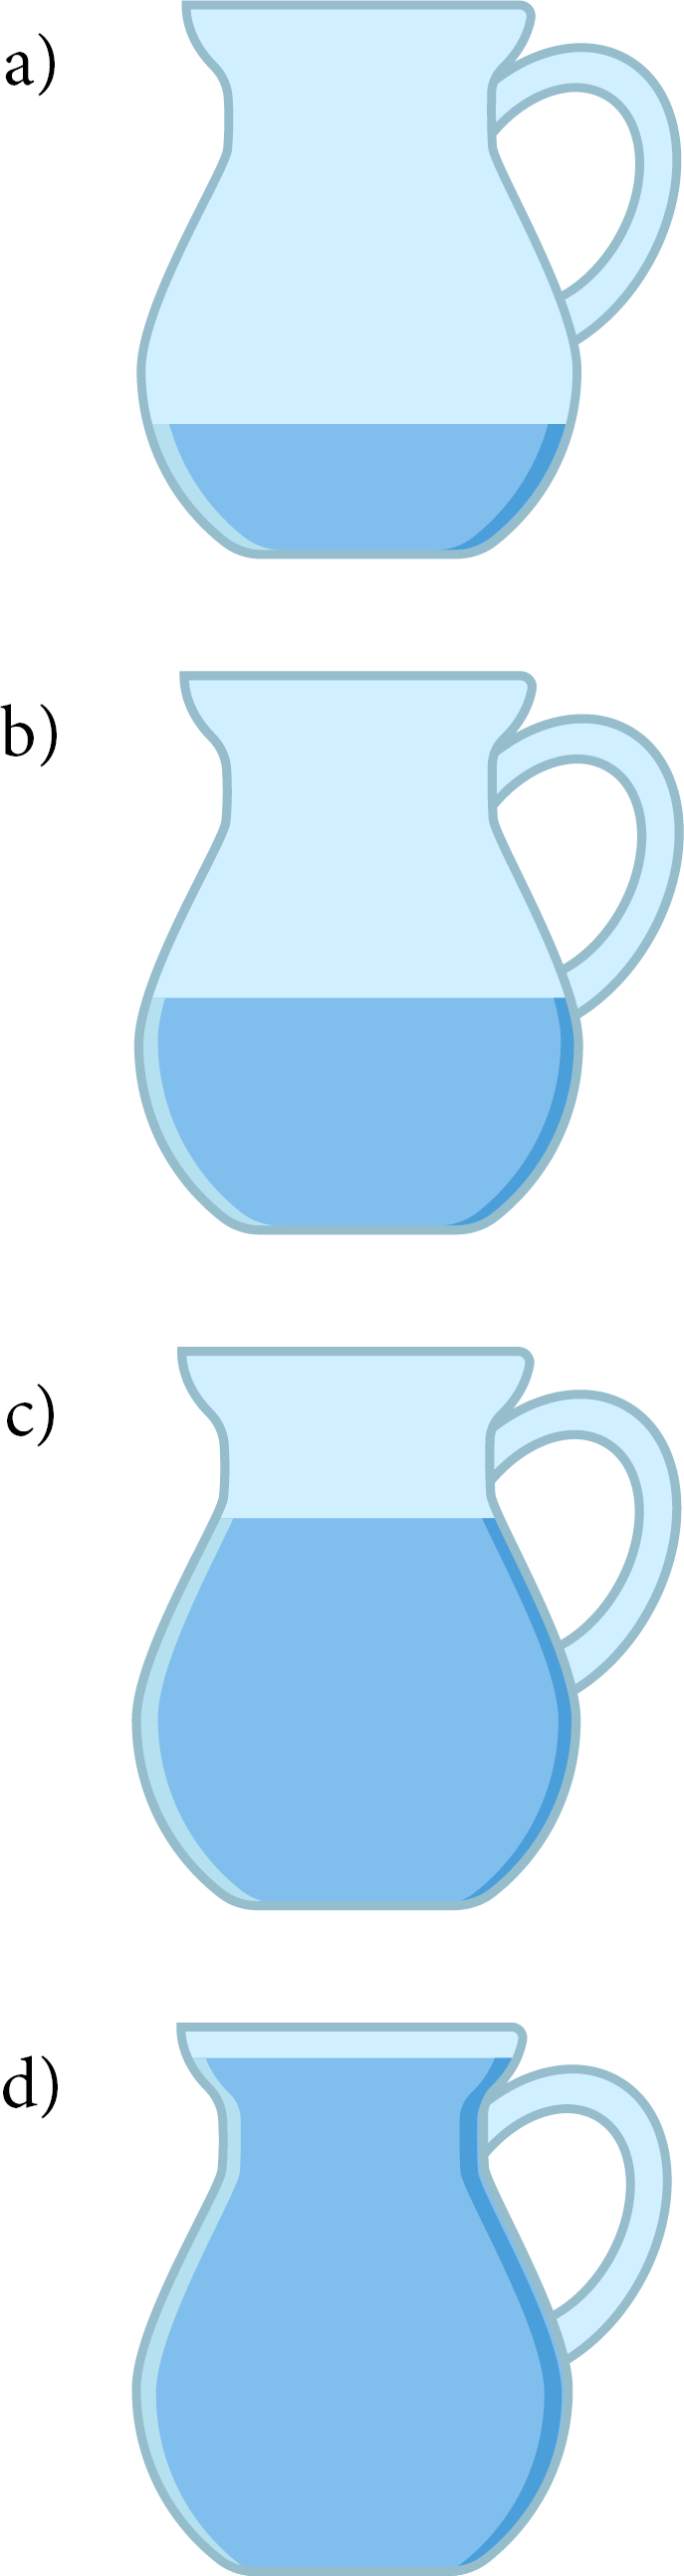
\includegraphics[width=.2\textwidth]{./media/image141.png}
\end{figure}

\num{7} Indique a sequência de figuras que apresenta a ordem em que normalmente as
atividades diárias acontecem.

\begin{figure}[H]
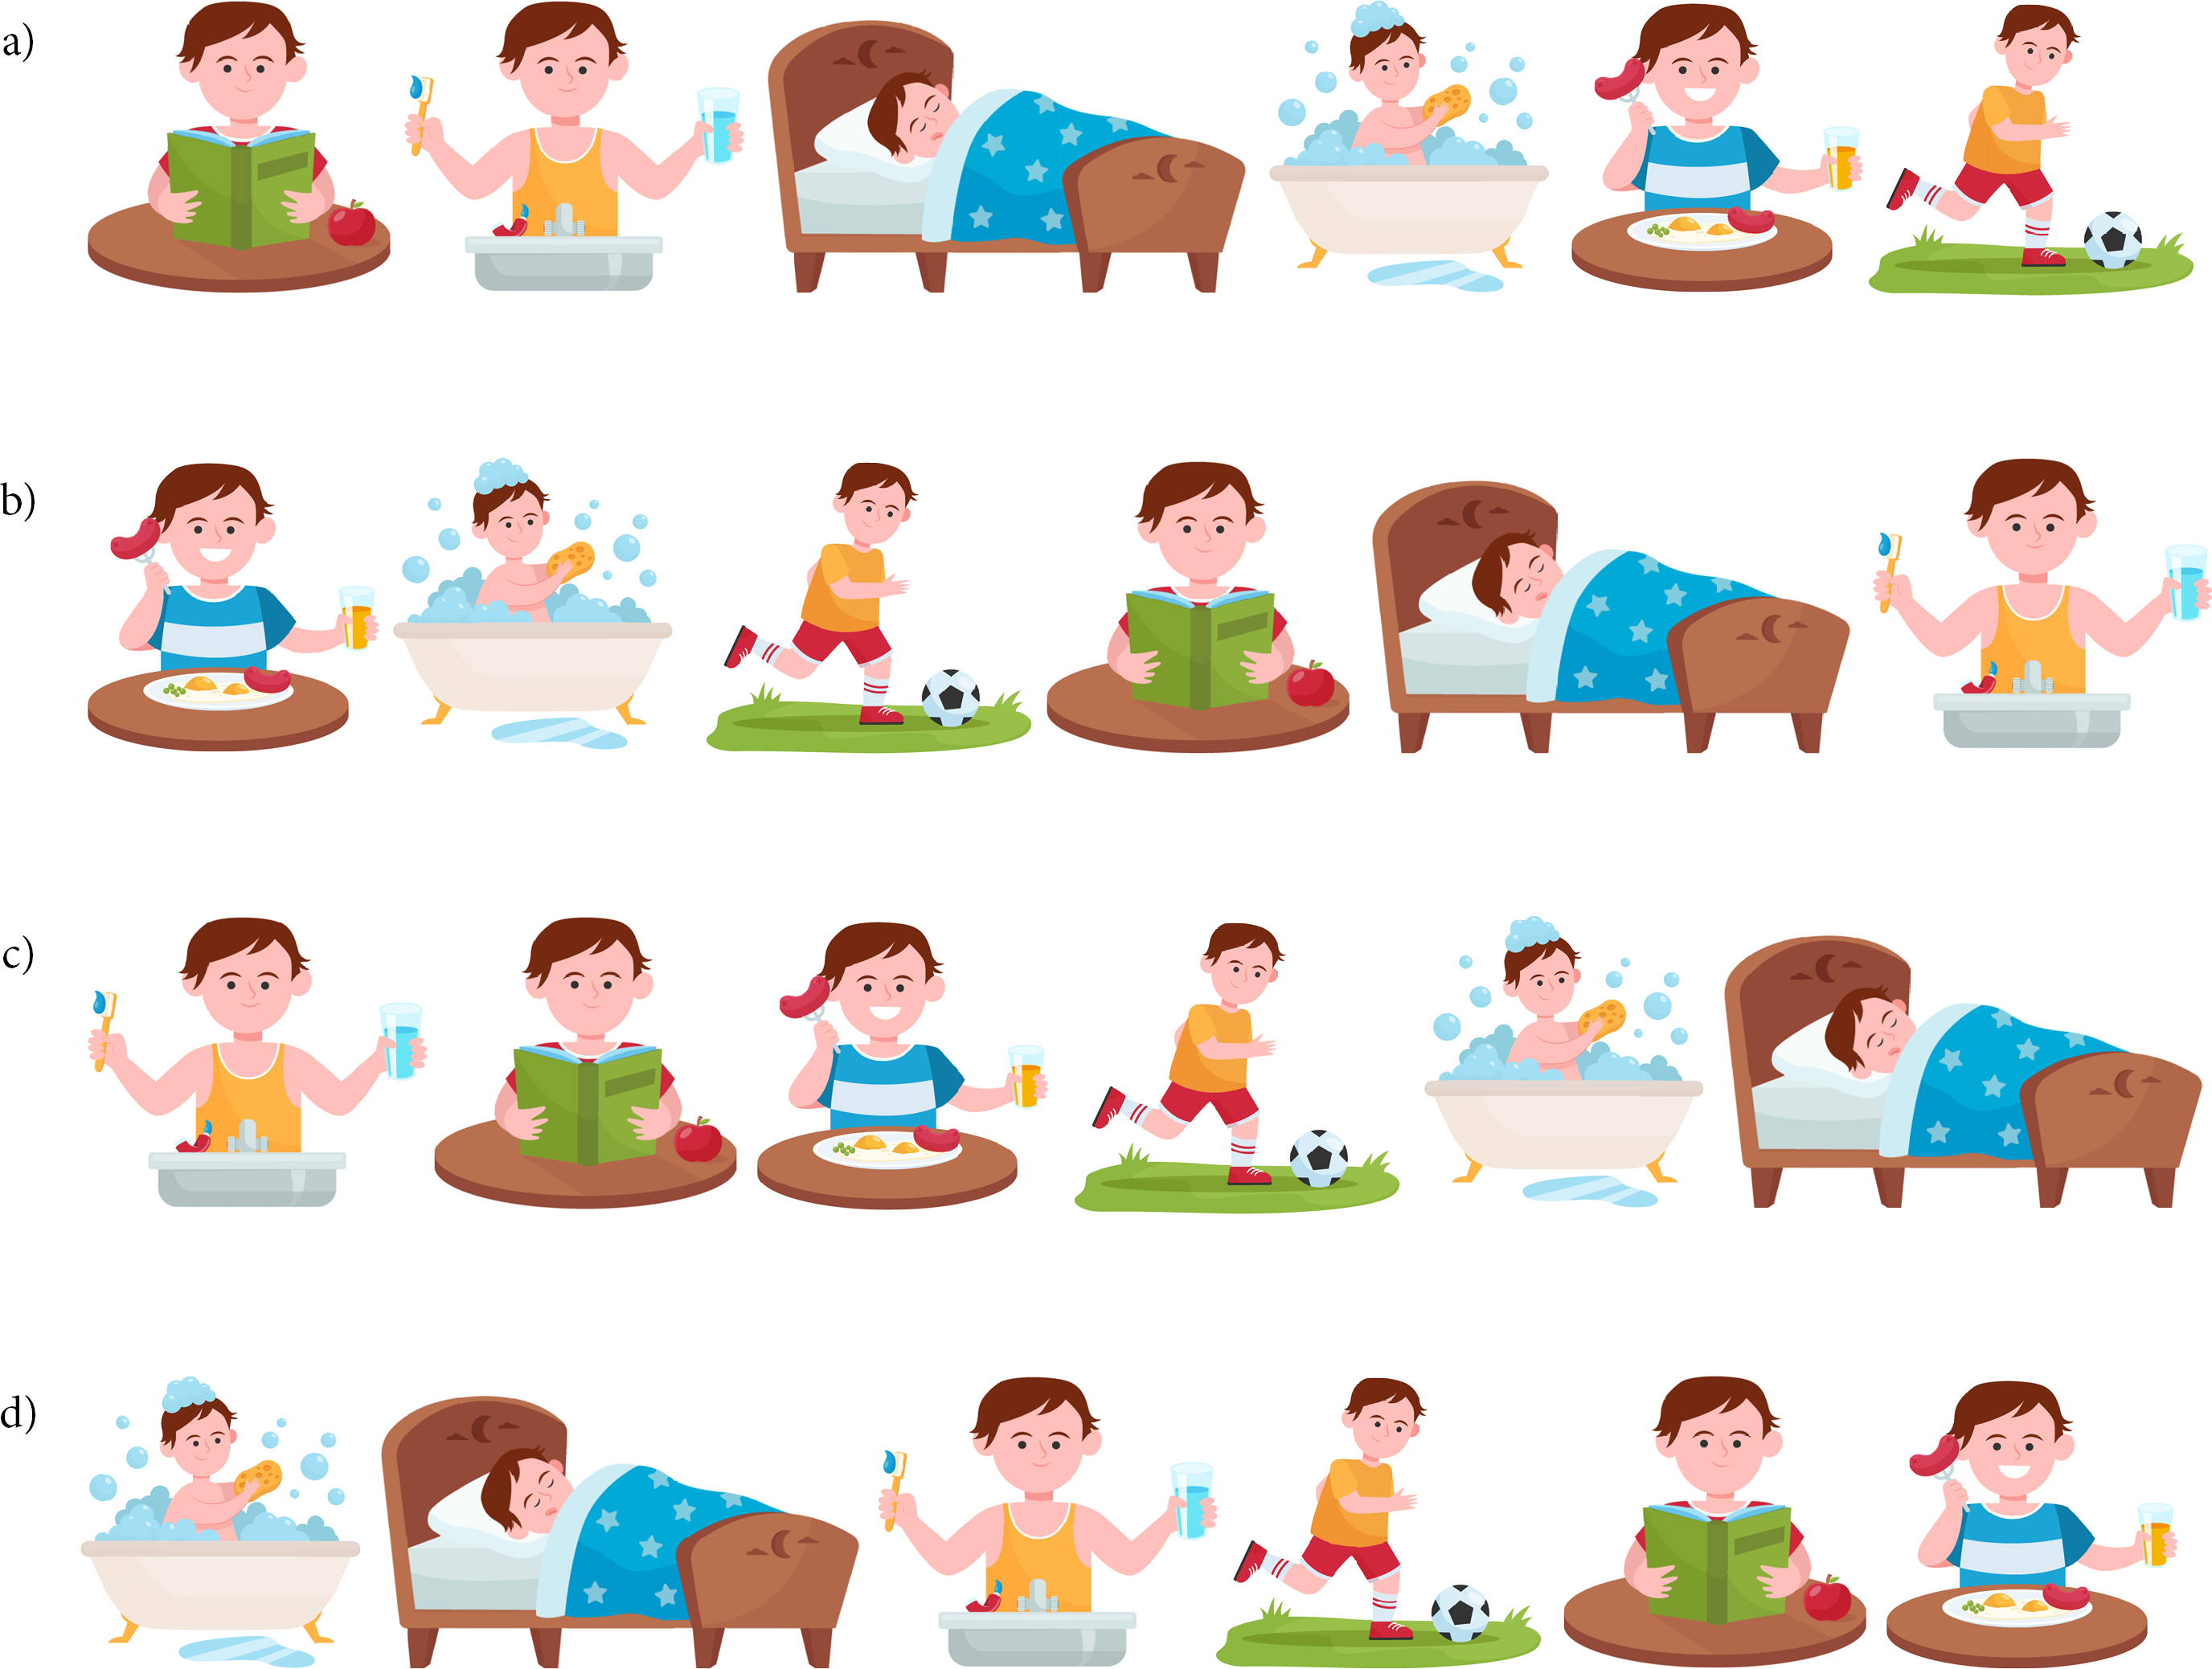
\includegraphics[width=\textwidth]{./media/image142.png}
\end{figure}


\num{8} Beatriz é uma mãe que sempre dá frutas para seu filho comer. Ela
montou uma tabela, para que seu filho coma uma fruta diferente a cada
dia da semana.

\begin{figure}[H]
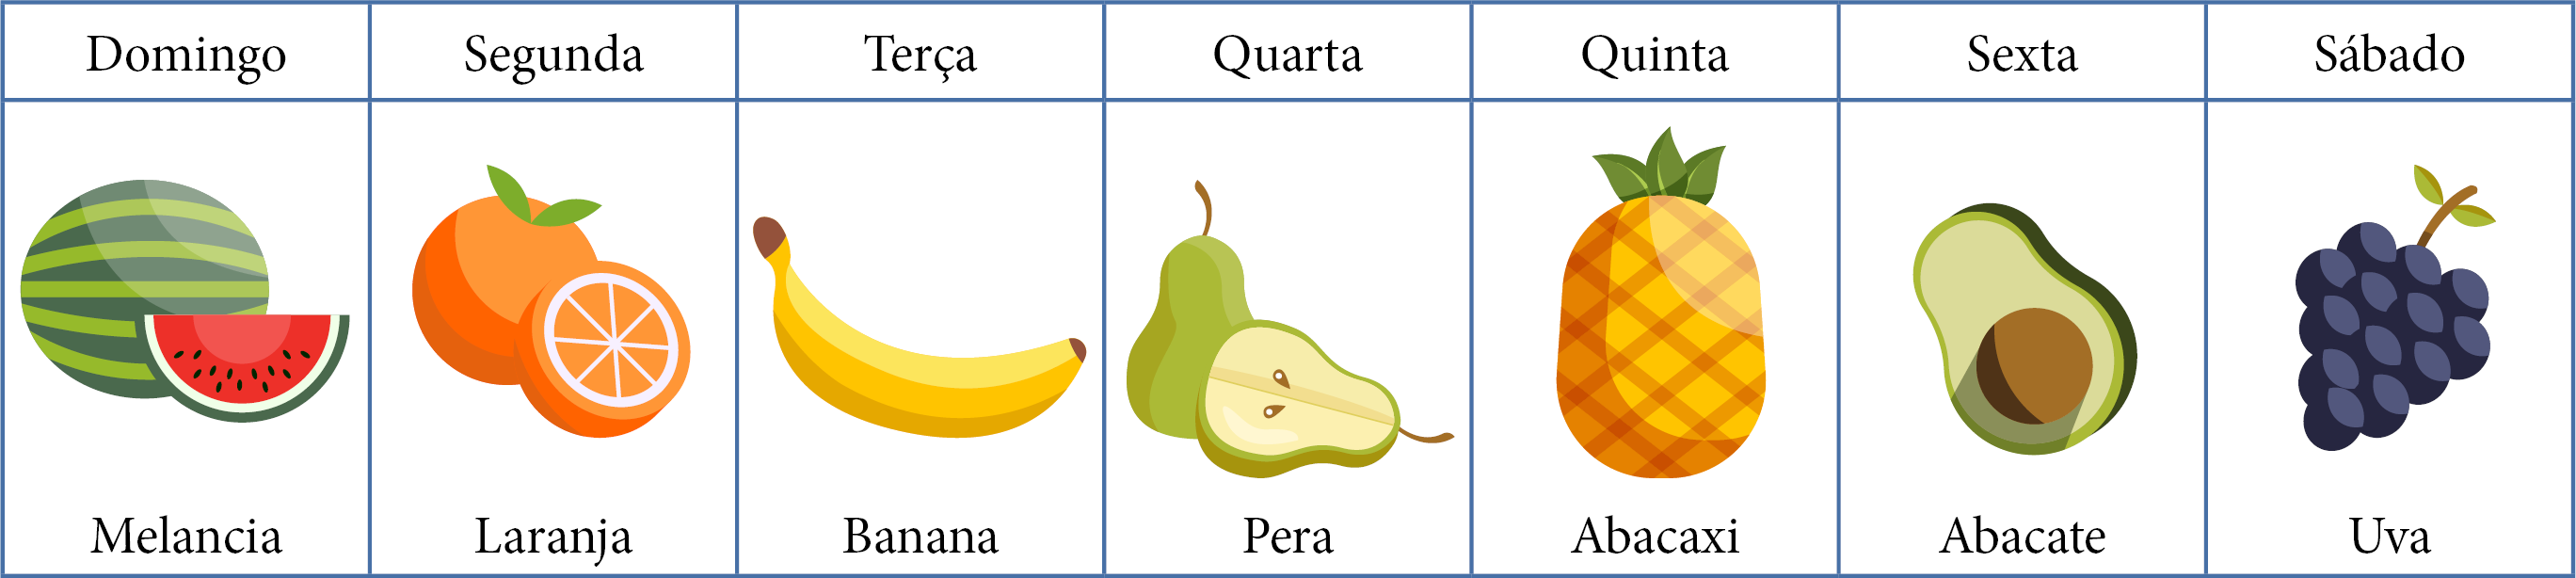
\includegraphics[width=\textwidth]{./media/image143.png}
\end{figure}

Observe o calendário do ano de 2023 e indique qual fruta o filho de
Beatriz irá comer, considerando que ela consiga seguir o planejamento, no dia 6 de julho.

\begin{figure}[H]
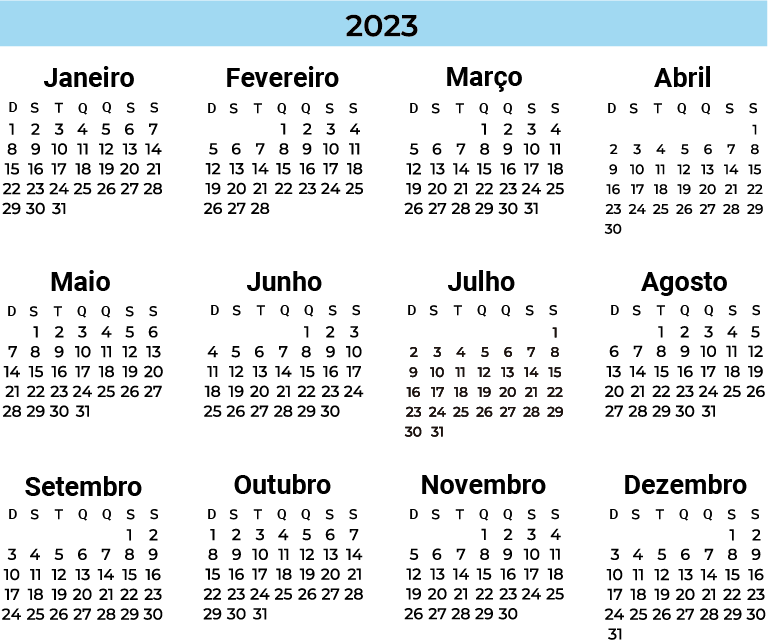
\includegraphics[width=\textwidth]{./media/image144.png}
\end{figure}

\begin{escolha}[itemsep=-5pt]
\item Abacaxi.

\item Banana.

\item Laranja.

\item Pera.
\end{escolha}

\num{9} Brenda foi à padaria com sua mãe e comprou algumas guloseimas para o
lanche da tarde. Observe as cédulas que a mãe de Brenda usou para pagar
o lanche e indique o valor que elas gastaram na padaria.

\begin{figure}[H]
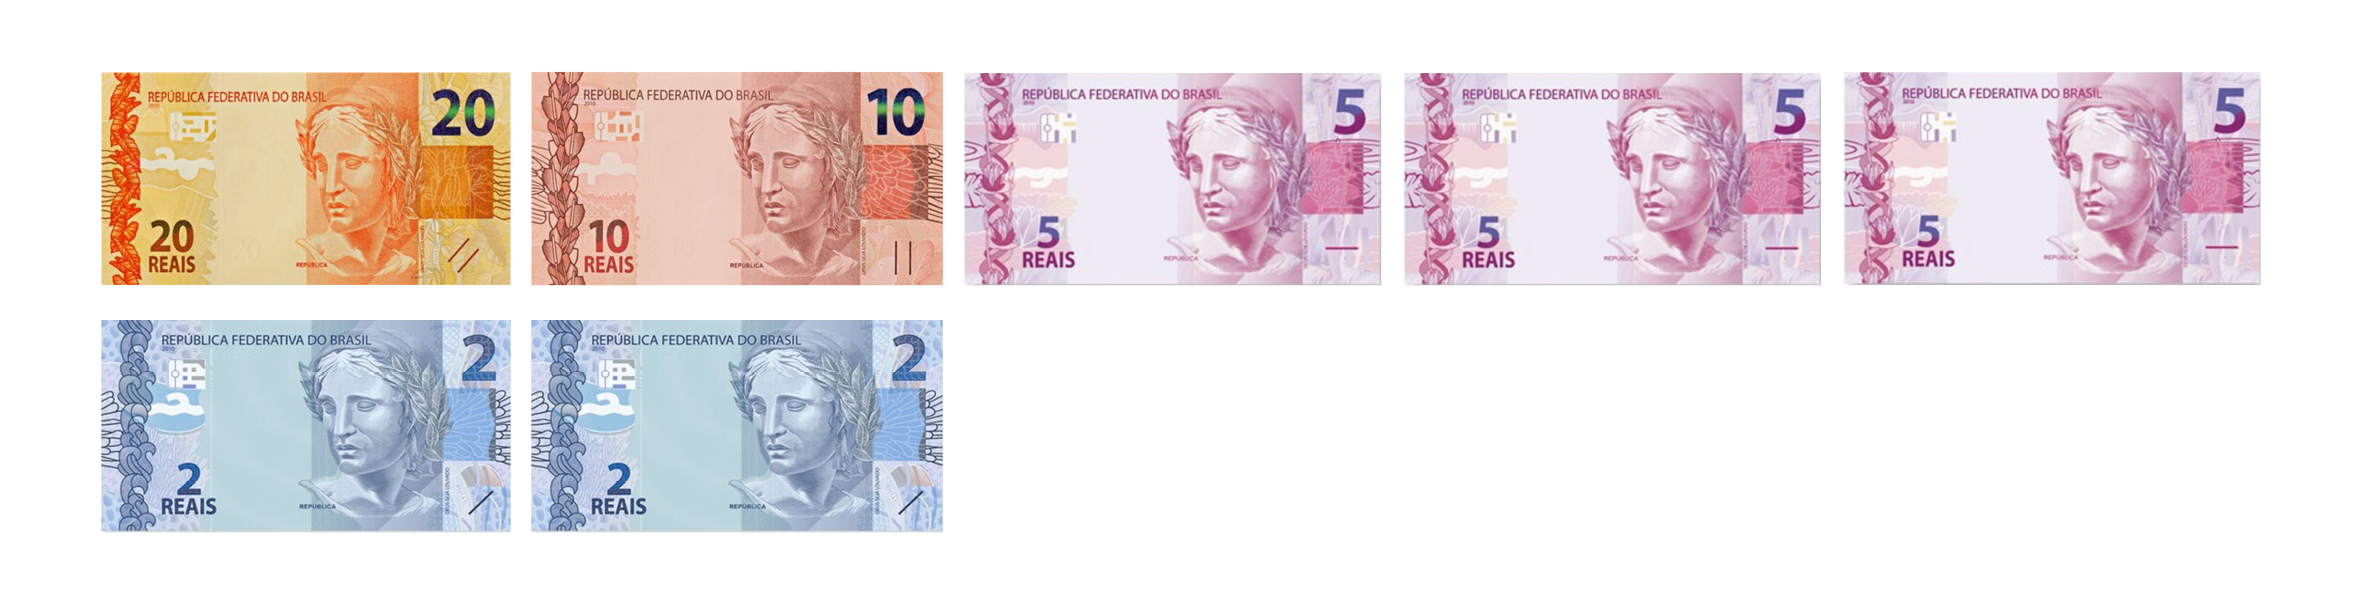
\includegraphics[width=\textwidth]{./media/image145.png}
\end{figure}

\begin{escolha}[itemsep=-5pt]
\item 37 reais.

\item 42 reais.

\item 49 reais.

\item 54 reais.
\end{escolha}

\num{10} Lúcia foi ao caixa eletrônico sacar o valor de 160 reais. Observe a seguir
as cédulas disponíveis no caixa eletrônico e marque uma das
possibilidades de notas que poderiam ser sacadas.

\begin{figure}[H]
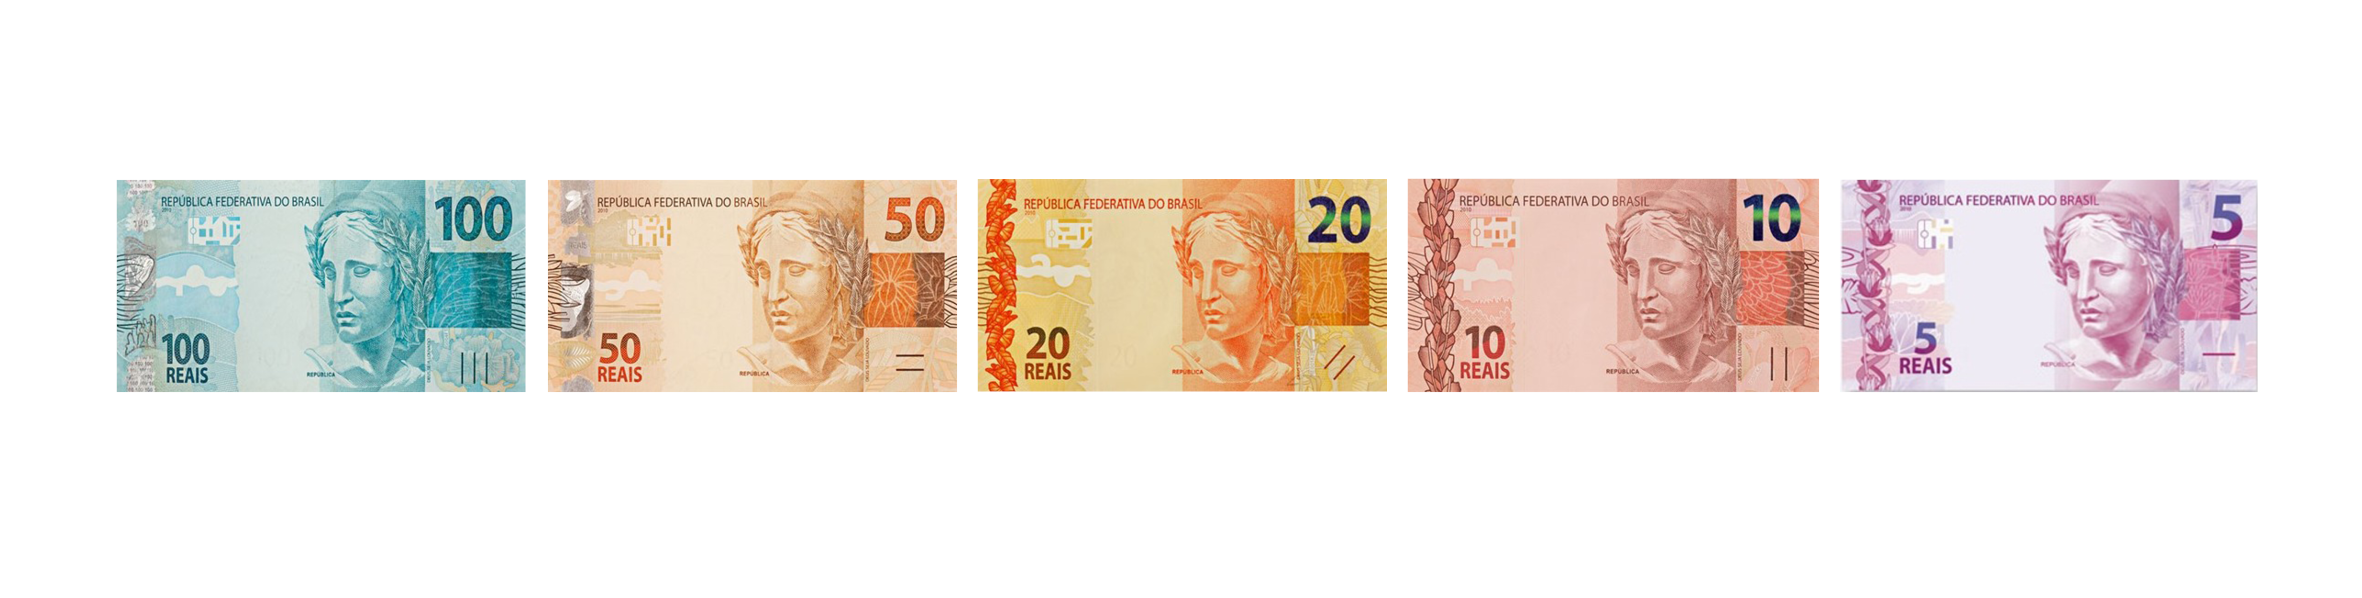
\includegraphics[width=\textwidth]{./media/image146.png}
\end{figure}

\begin{escolha}[itemsep=-5pt]
\item 6 cédulas de 20 reais, 1 cédula de 50 reais e 1 cédula de 10 reais.

\item 3 cédulas de 50 reais, 1 cédula de 20 reais e 1 cédula de 5 reais.

\item 2 cédulas de 50 reais, 2 cédulas de 10 reais e 2 cédulas de 5 reais.

\item 1 cédula de 100 reais, 1 cédula de 50 reais e 1 cédula de 10 reais.
\end{escolha}

\num{11} José e Ana brincam em uma piscina de bolinhas; dentre outras cores, há
na piscina 400 bolinhas verdes, 400 amarelas e 350 vermelhas, sendo
essas três cores as mais presentes na piscina.

\begin{figure}[H]
\centering
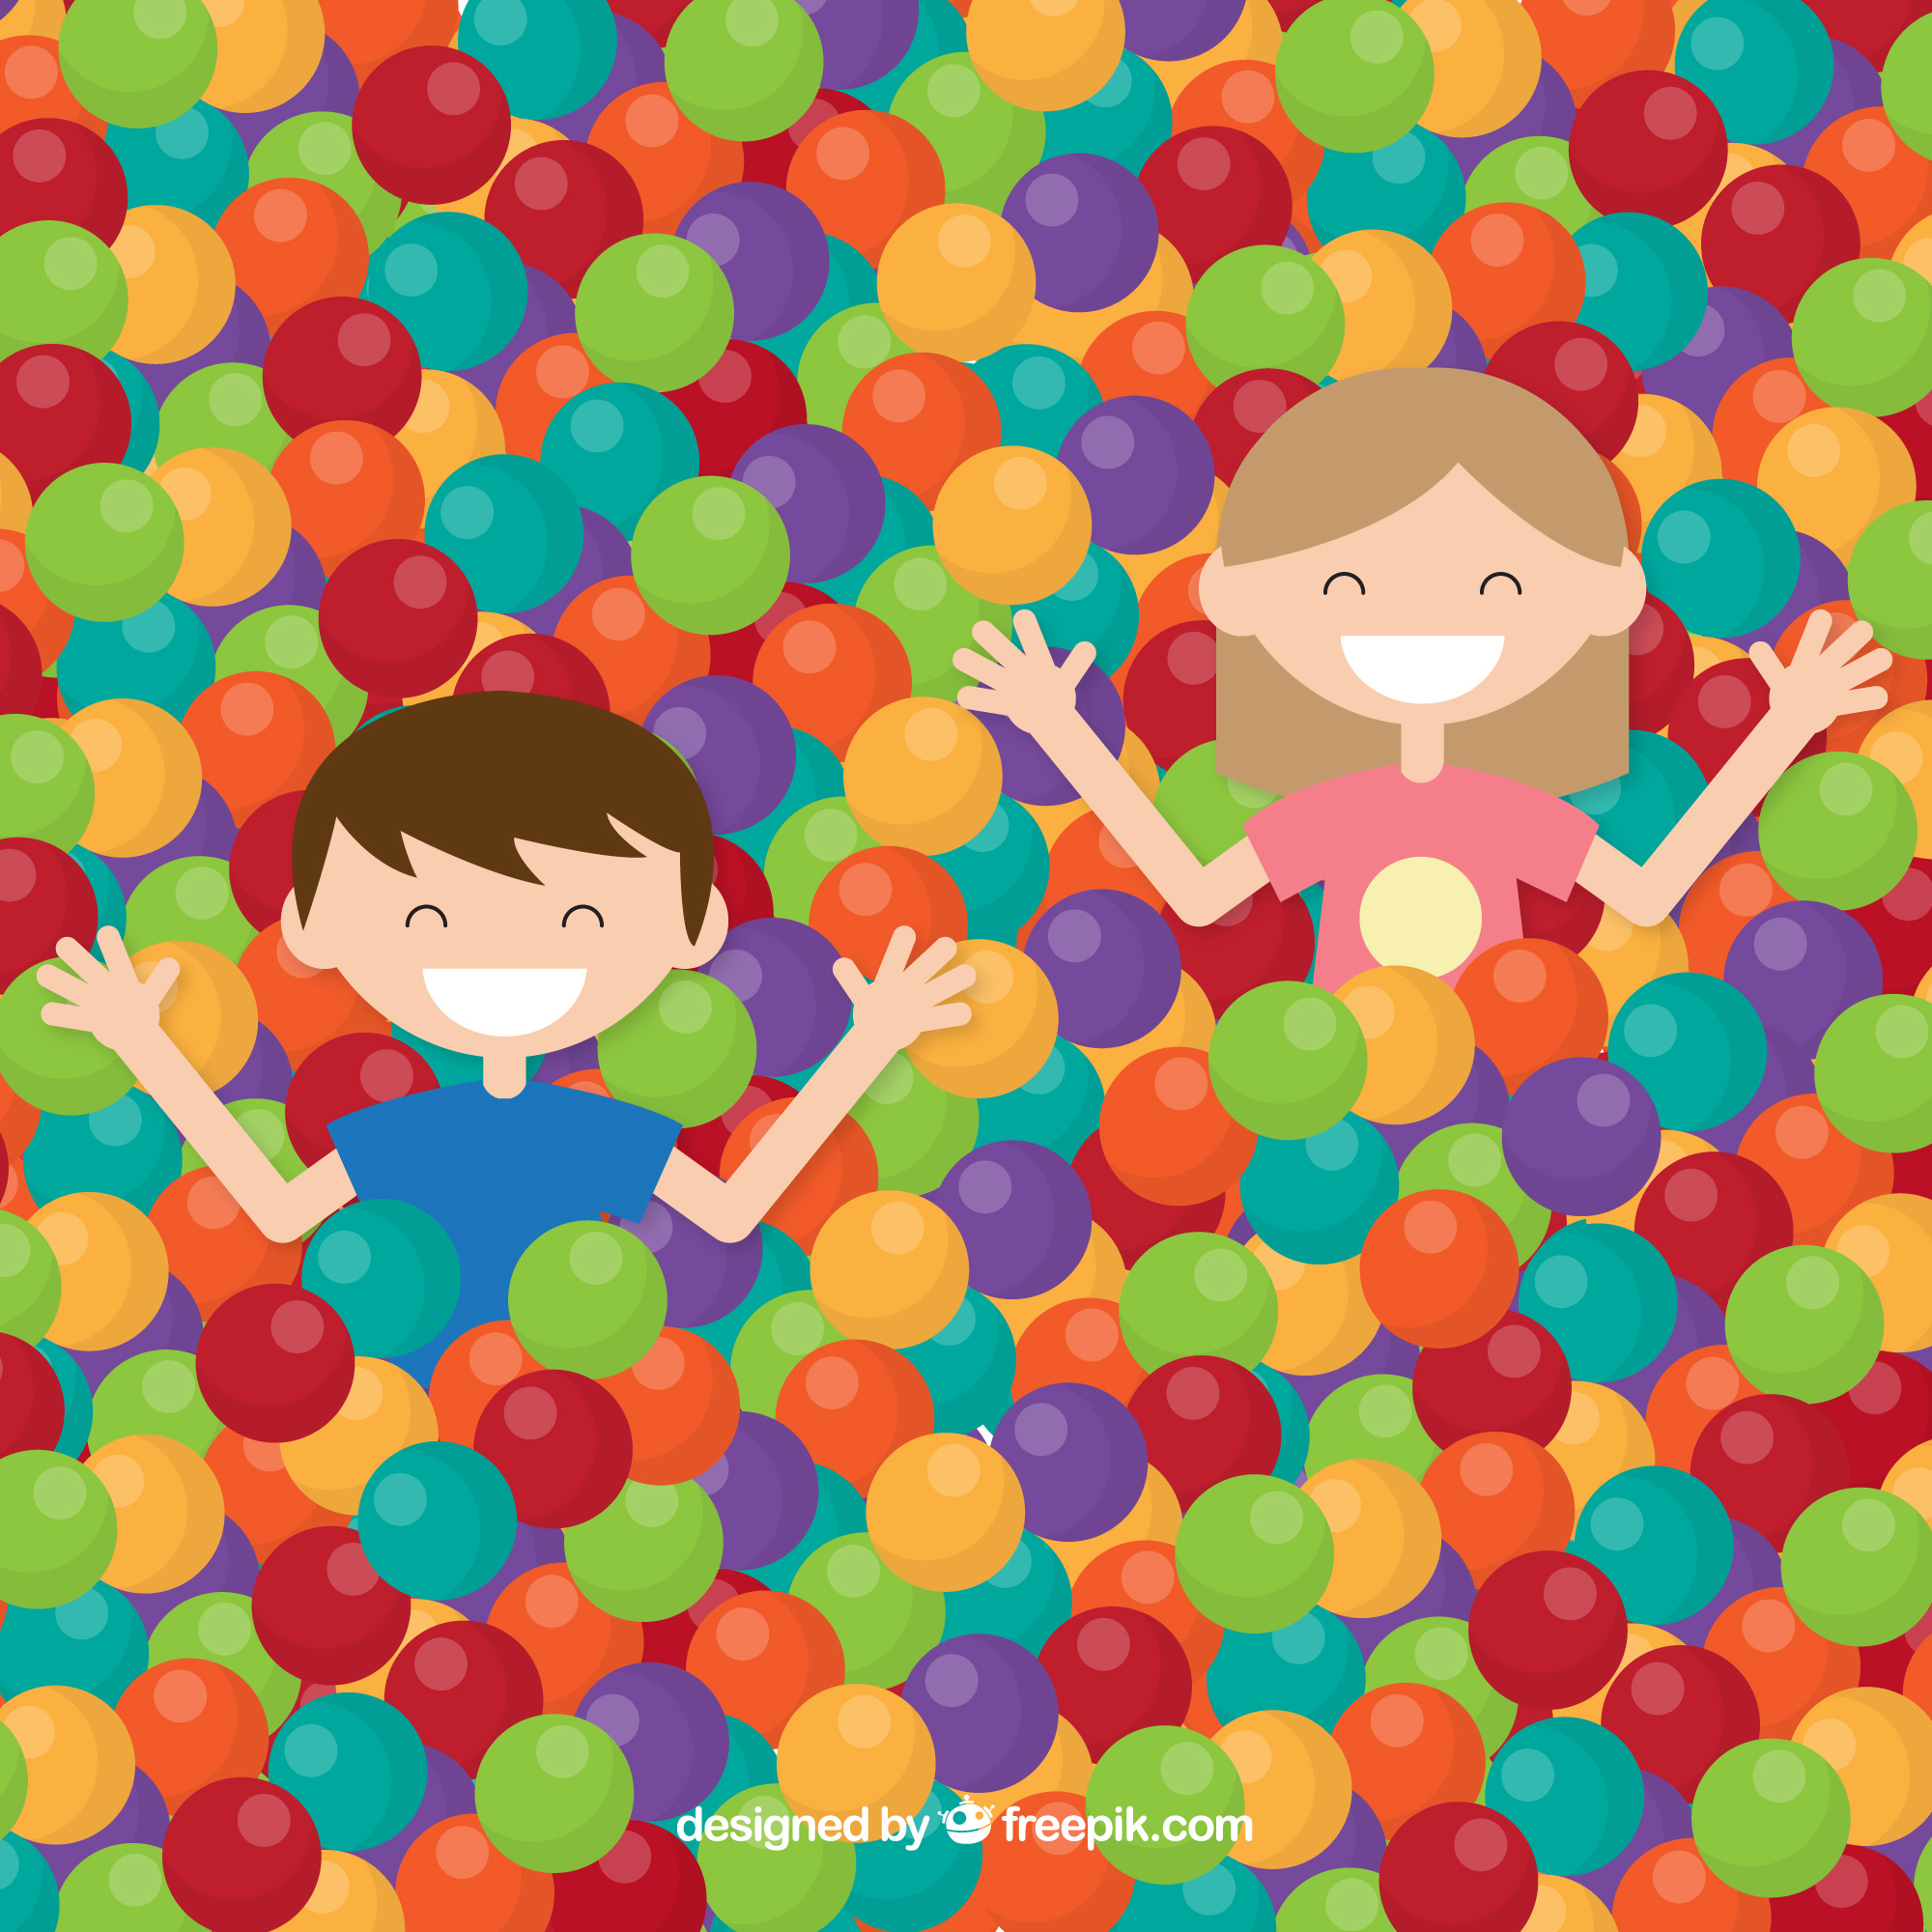
\includegraphics[width=.5\textwidth]{./media/image147.png}
\end{figure}

A brincadeira consiste em pegar aleatoriamente as bolinhas uma a uma e
arremessar em um alvo fora da piscina. Sobre as bolinhas arremessadas, o que se pode afirmar?

\begin{escolha}[itemsep=-5pt]
\item É muito provável que as bolinhas arremessadas sejam todas verdes.

\item É provável que a maior parte das bolinhas arremessadas sejam verdes e amarelas.

\item É impossível serem arremessadas bolinhas vermelhas.

\item É certo que, em 3 lançamentos, seja arremessada uma bolinha de cada cor indicada.
\end{escolha}

\num{12} A tabela a seguir mostra o preço de alguns produtos da vendinha da escola.

\begin{figure}[H]
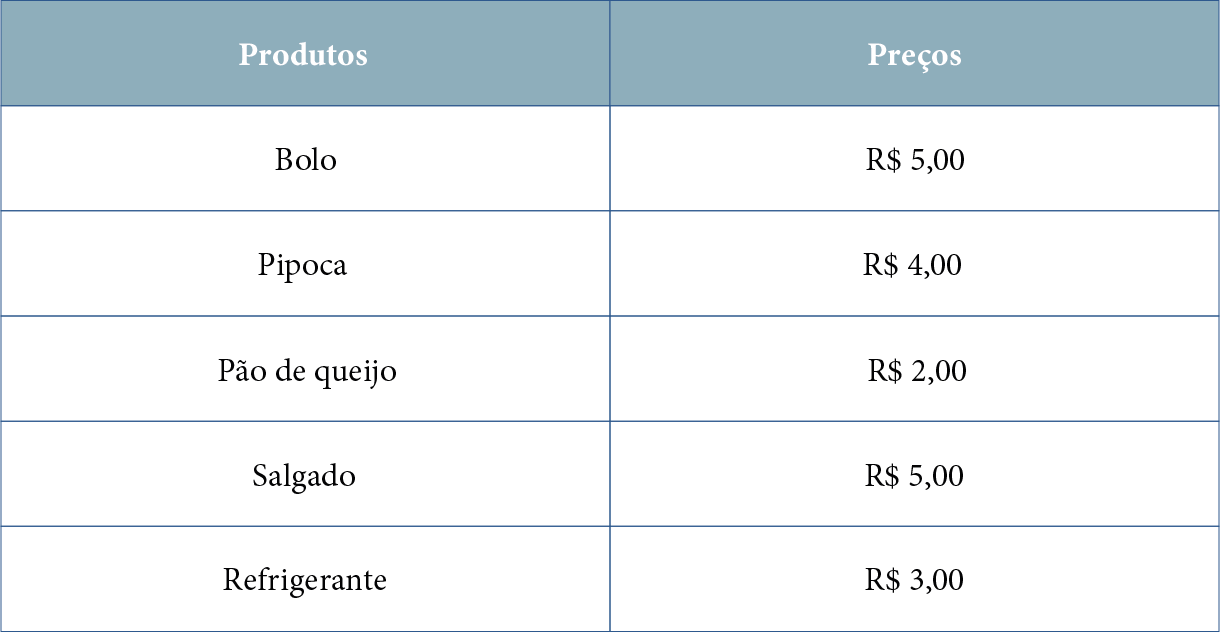
\includegraphics[width=\textwidth]{./media/image148.png}
\end{figure}

Quanto Tiago vai pagar na vendinha se comer um bolo, um pão de queijo e um refrigerante?

\begin{escolha}[itemsep=-5pt]
\item R\$ 5,00

\item R\$ 8,00

\item R\$ 10,00

\item R\$ 13,00
\end{escolha}

\num{13} O gráfico a seguir mostra o resultado de uma pesquisa sobre a matéria de
preferência dos estudantes do 2º ano. Qual a matéria preferida entre eles?

\begin{figure}[H]
\centering
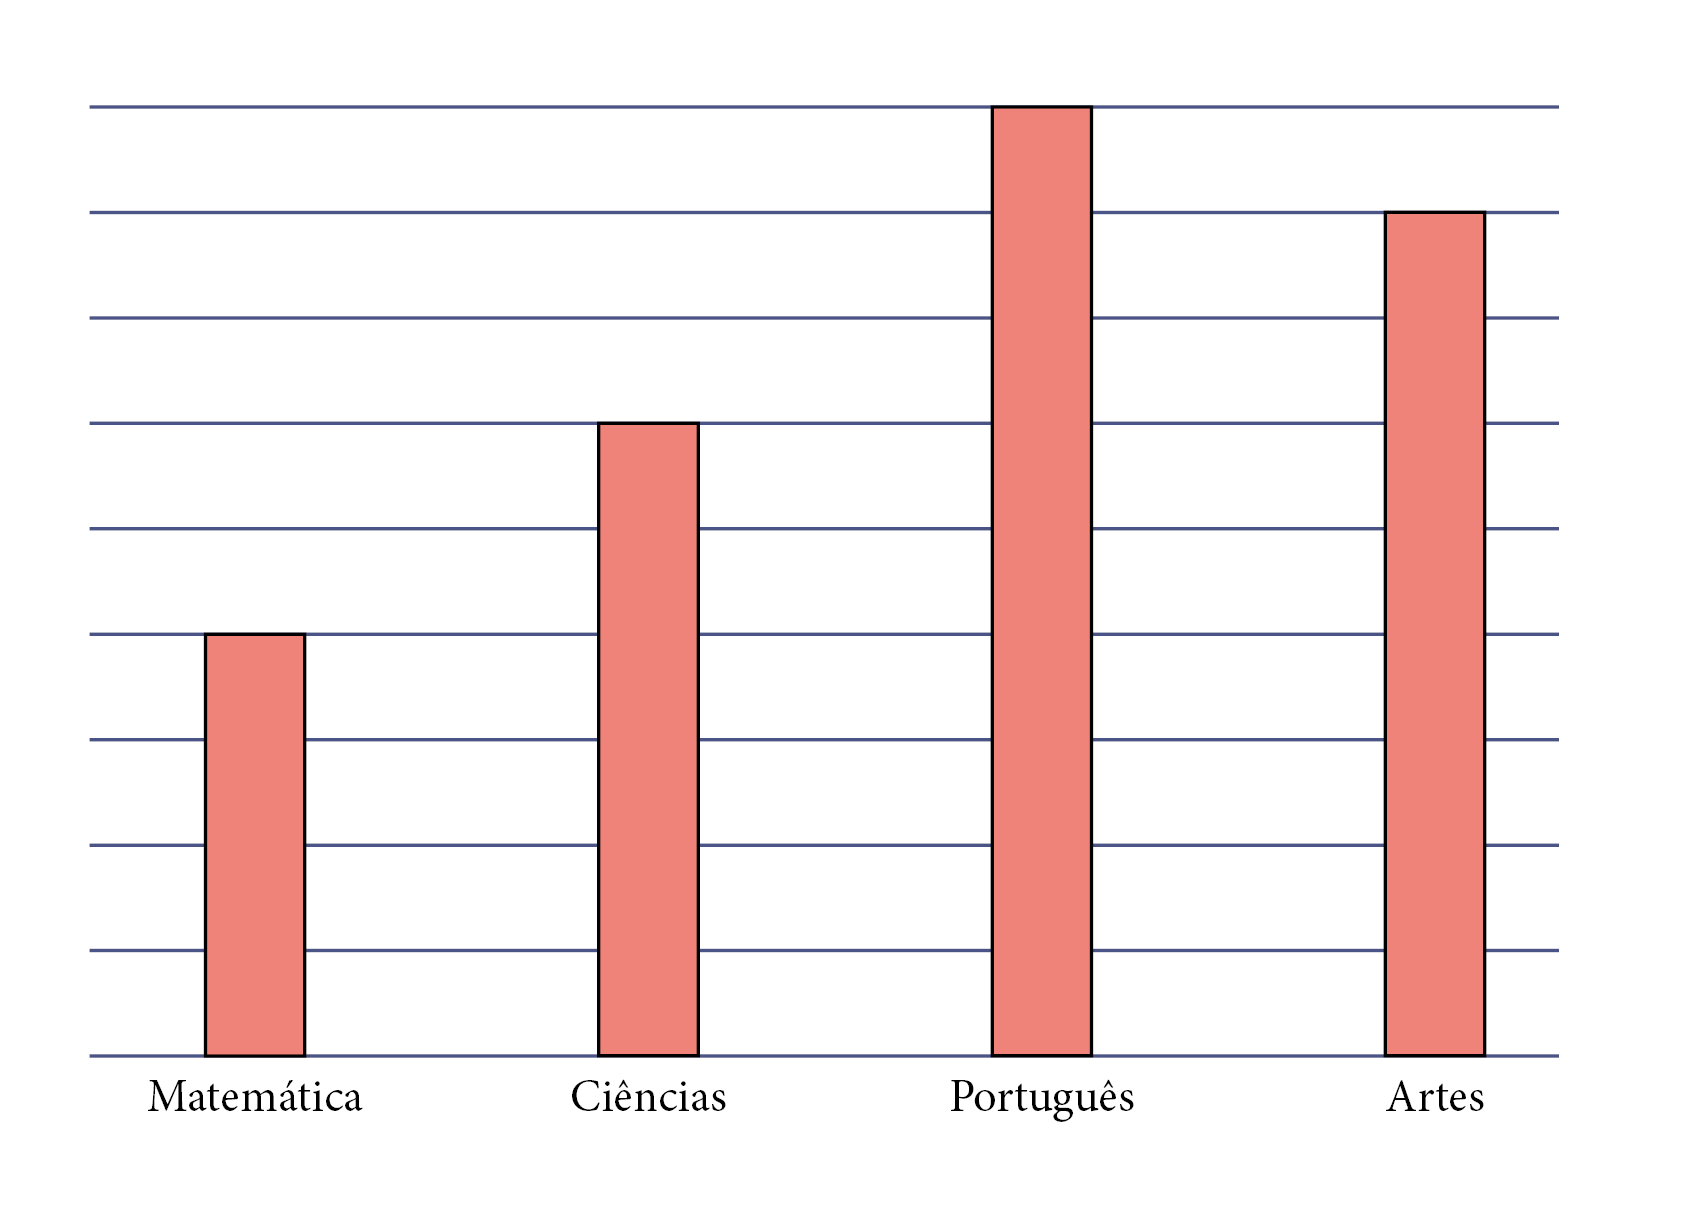
\includegraphics[width=\textwidth]{./media/image149.png}
\end{figure}

\begin{escolha}[itemsep=-5pt]
\item Artes

\item Ciências

\item Matemática

\item Português
\end{escolha}

\num{14} Kátia fez 9 cupcakes com diferentes sabores: 3 de mirtilo, 3 de morango
e 3 de creme. Sendo assim, é correto afirmar que:

% \begin{figure}[H]
% \centering
% 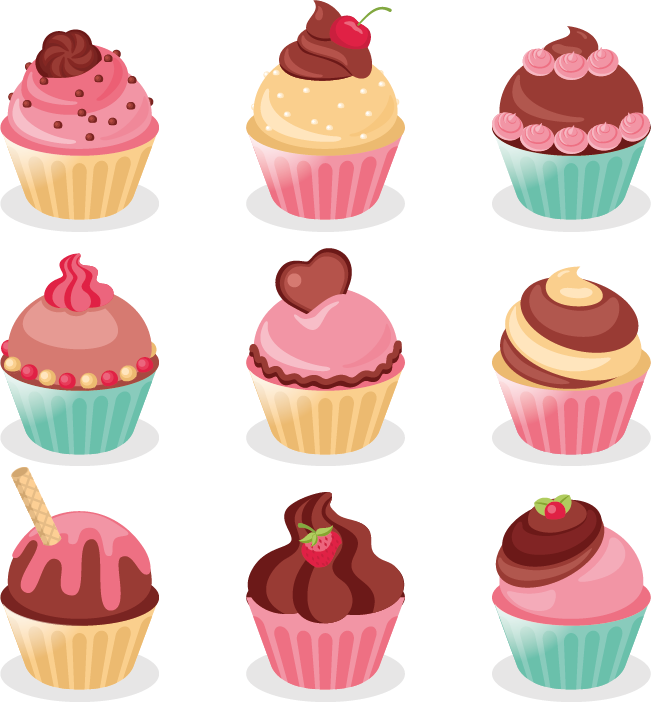
\includegraphics[width=.4\textwidth]{./media/image150.png}
% \end{figure}

\begin{escolha}[itemsep=-5pt]
\item Metade dos cupcakes são de mirtilo.

\item Os cupcakes de creme são o dobro dos cupcakes de mirtilo.

\item Um quarto dos cupcakes são de creme.

\item Um terço dos cupcakes são de morango.
\end{escolha}


\num{15} O senhor João tem uma fazenda com várias vacas e sua principal fonte de renda é a venda do leite em garrafas de 2 litros. Quantas
garrafas ele irá vender, sendo que tirou 256 litros de leite?

\begin{escolha}[itemsep=-5pt]
\item 128

\item 133

\item 153

\item 256
\end{escolha}

\chapter[Simulado 4]{Simulado}
\markboth{Simulado 4}{}

\num{1} A placa presente na imagem mostra o limite máximo de velocidade de uma
rodovia. Marque a alternativa que apresenta corretamente como se escreve
esse número por extenso.

\begin{figure}[H]
\centering
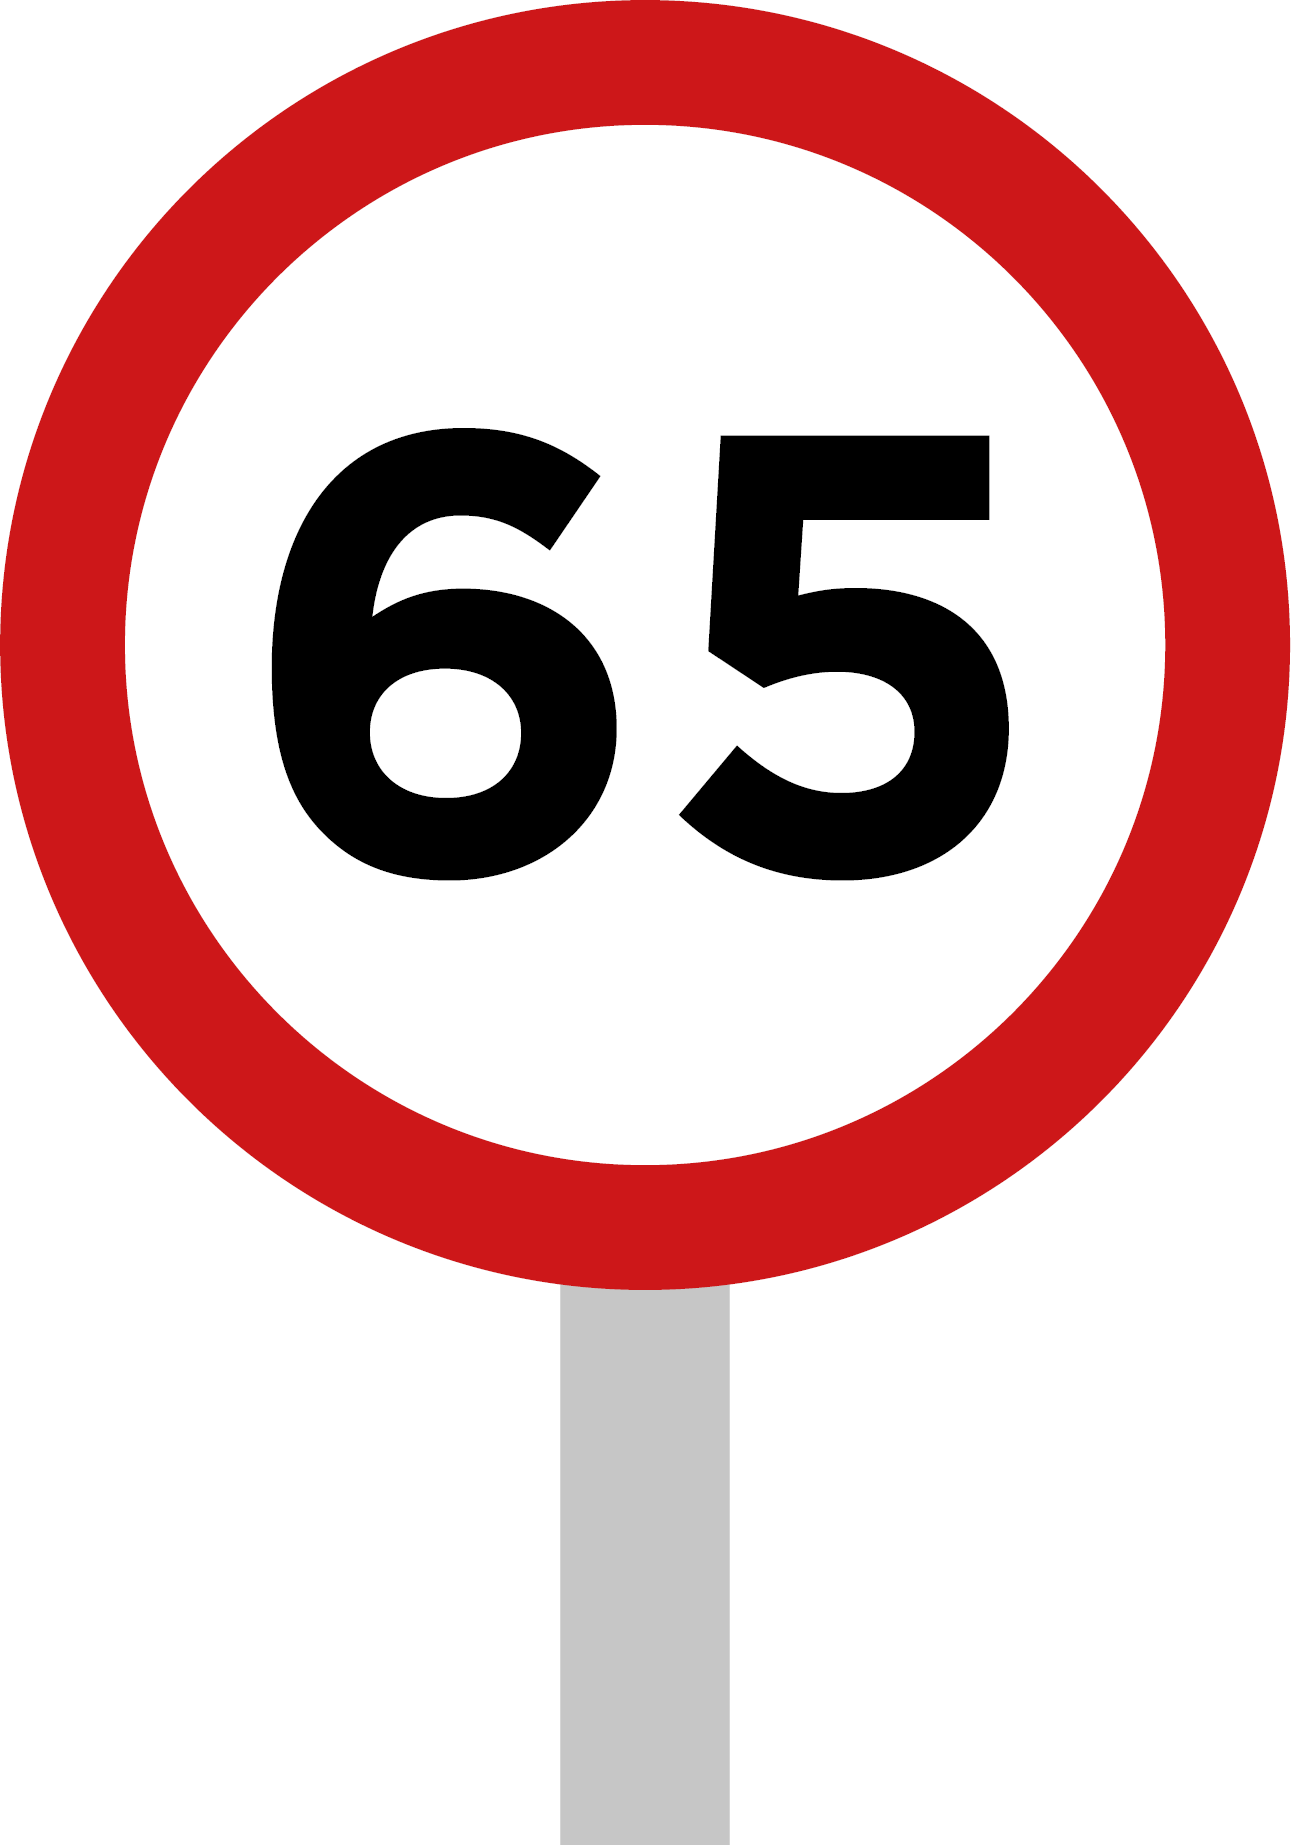
\includegraphics[width=.25\textwidth]{./media/image151.png}
\end{figure}

\begin{escolha}[itemsep=-5pt]
\item Seis e cinco

\item Seiscentos e cinco

\item Sessenta e cinco

\item Setenta e cinco
\end{escolha}

\num{2} Laura comprou duas caixas de macaron, que é um tipo de biscoito colorido
francês, para presentear suas amigas. 

\begin{figure}[H]
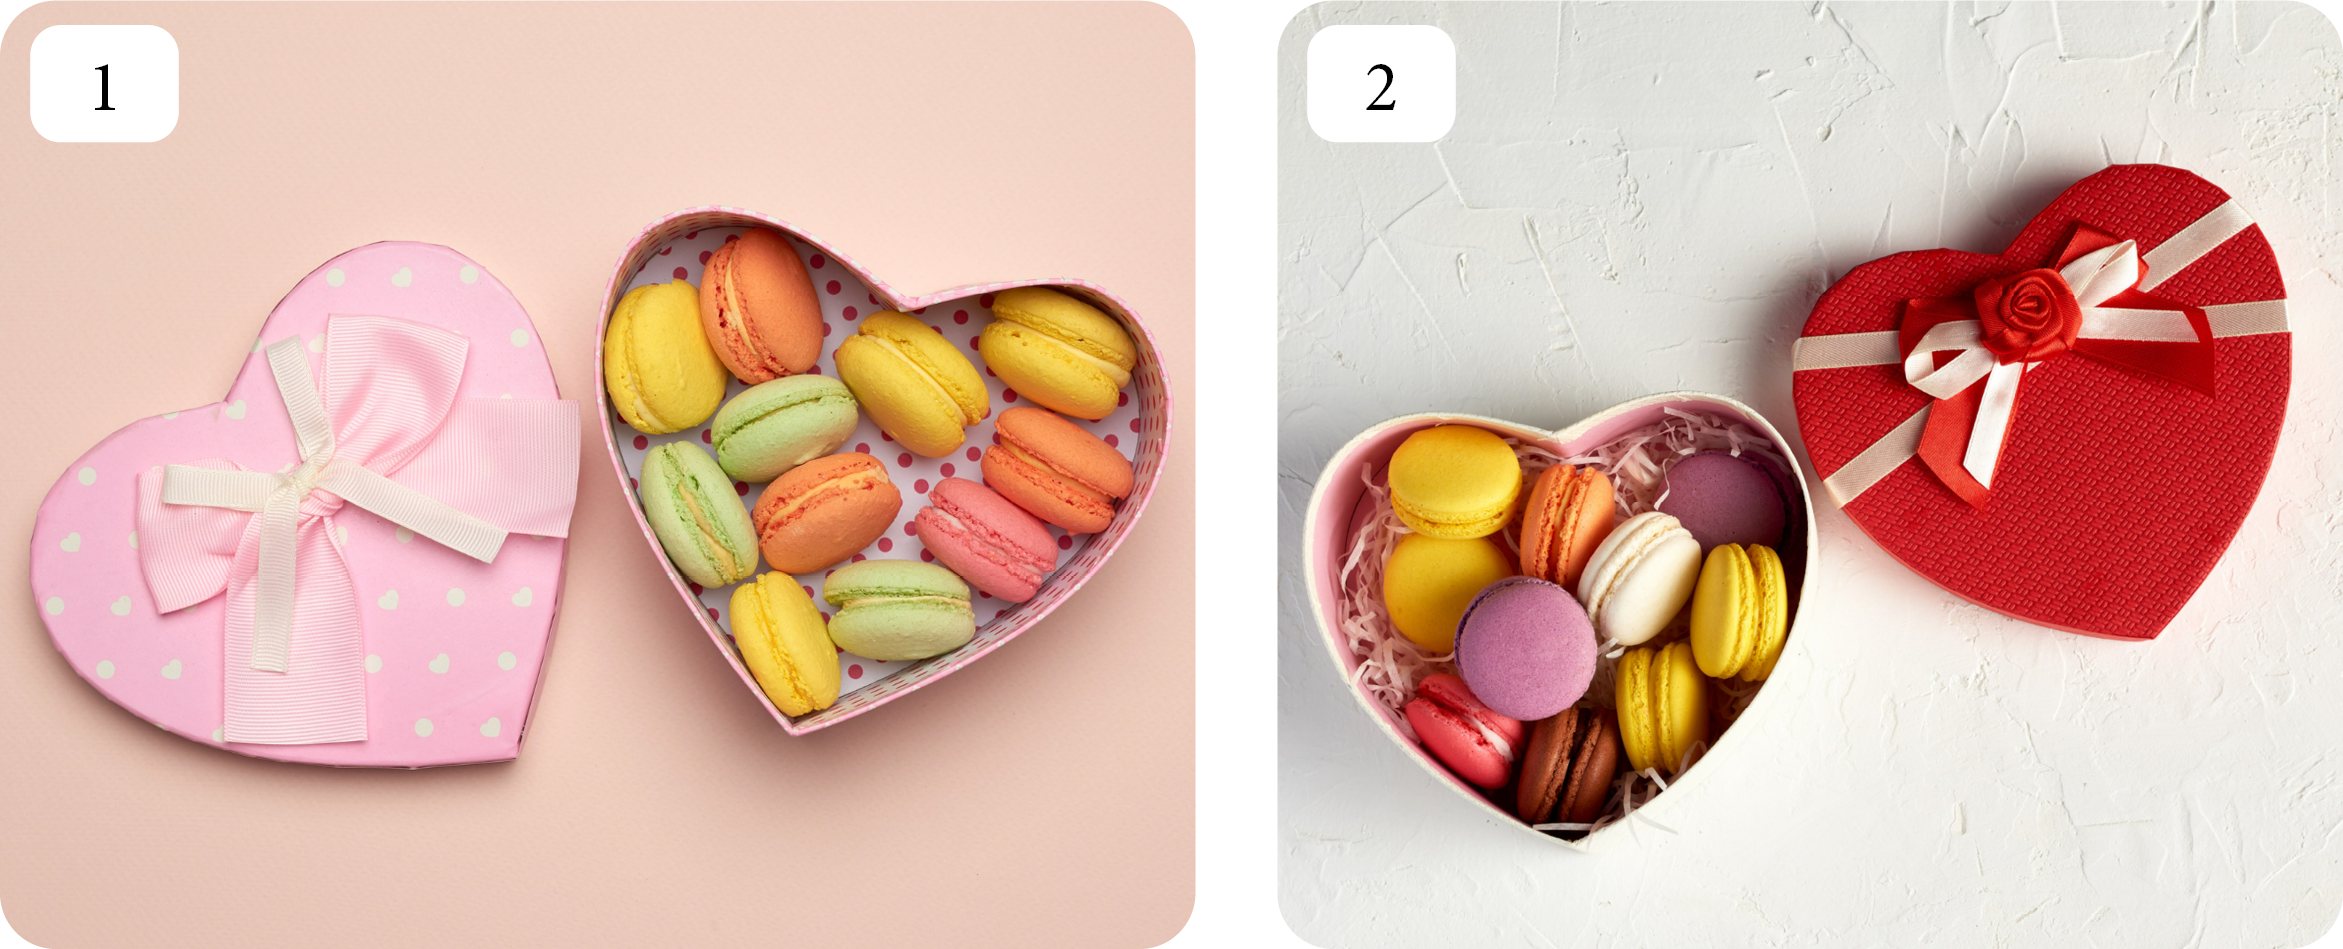
\includegraphics[width=\textwidth]{./media/image152.png}
\end{figure}

Examine as caixas e marque a
alternativa que contém a resposta correta sobre elas.

\begin{escolha}[itemsep=-5pt]
\item A caixa 1 tem cinco macarons a mais do que a caixa 2.

\item A caixa 2 tem dois macarons a mais do que a caixa 1.

\item A caixa 2 tem um macaron a menos do que a caixa 1.

\item As caixas 1 e 2 têm a mesma quantidade de macarons.
\end{escolha}

\num{3} Indique qual das subtrações a seguir pode ter como resultado o número 75.

\begin{escolha}[itemsep=-5pt]
\item 280 -- 120 -- 60 -- 25.

\item 250 -- 45 -- 55 -- 85.

\item 220 -- 75 -- 40 -- 20.

\item 200 -- 65 -- 50 -- 30.
\end{escolha}

\num{4} Uma professora vai distribuir guloseimas para seus alunos no Dia das
Crianças. Ela pretende colocar 5 guloseimas em cada pacotinho. Quantas
guloseimas ela precisa no total para montar os pacotes dos seus 12
alunos?

\begin{escolha}[itemsep=-5pt]
\item 50

\item 55

\item 60

\item 65
\end{escolha}

\num{5} O instrumento da figura a seguir mede em qual unidade de medida?

\begin{figure}[H]
\centering

\includegraphics[width=.3\textwidth]{./media/image153.png}
\end{figure}

\begin{escolha}[itemsep=-5pt]
\item Centímetro.

\item Litro.

\item Metro.

\item Quilograma.
\end{escolha}

\num{6} Qual o melhor instrumento de medidas para pesar as frutas na frutaria do
senhor José?

\begin{figure}[H]
\centering
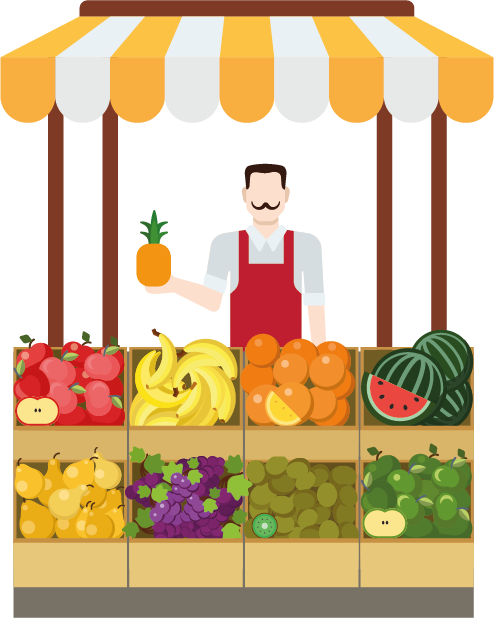
\includegraphics[width=.3\textwidth]{./media/image154.png}
\end{figure}

\begin{escolha}[itemsep=-5pt]
\item As mãos.

\item Balança.

\item Copo medidor.

\item Régua.
\end{escolha}

\num{7} Observe o calendário do mês de maio do ano de 2024. Rodrigo foi
convidado para um evento que acontecerá em Macapá, no último final de
semana do mês de maio, contando sábado e domingo. Quais serão os dias em que acontecerá o evento?

\begin{figure}[H]
\centering
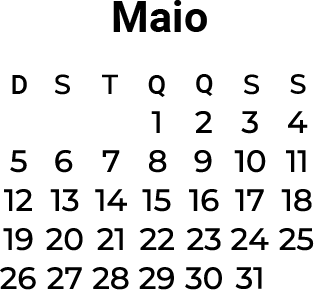
\includegraphics[width=.35\textwidth]{./media/image155.png}
\end{figure}

\begin{escolha}[itemsep=-5pt]
\begin{multicols}{2}
\item 4 e 5

\item 18 e 19

\item 25 a 26

\item 30 e 31
\end{multicols}
\end{escolha}

\num{8} Emanuel foi fazer algumas compras e acabou demorando bastante. Ele chegou ao mercado ao meio-dia e ficou lá por 2 horas e 35 minutos. Qual
o horário em que ele saiu do mercado?

\begin{escolha}[itemsep=-5pt]
\item 13:35

\item 14:05

\item 14:35

\item 15:05
\end{escolha}

\num{9} Observe a seguir o dinheiro que Raíssa tem e indique qual é o brinquedo que ela pode comprar.

\begin{figure}[H]
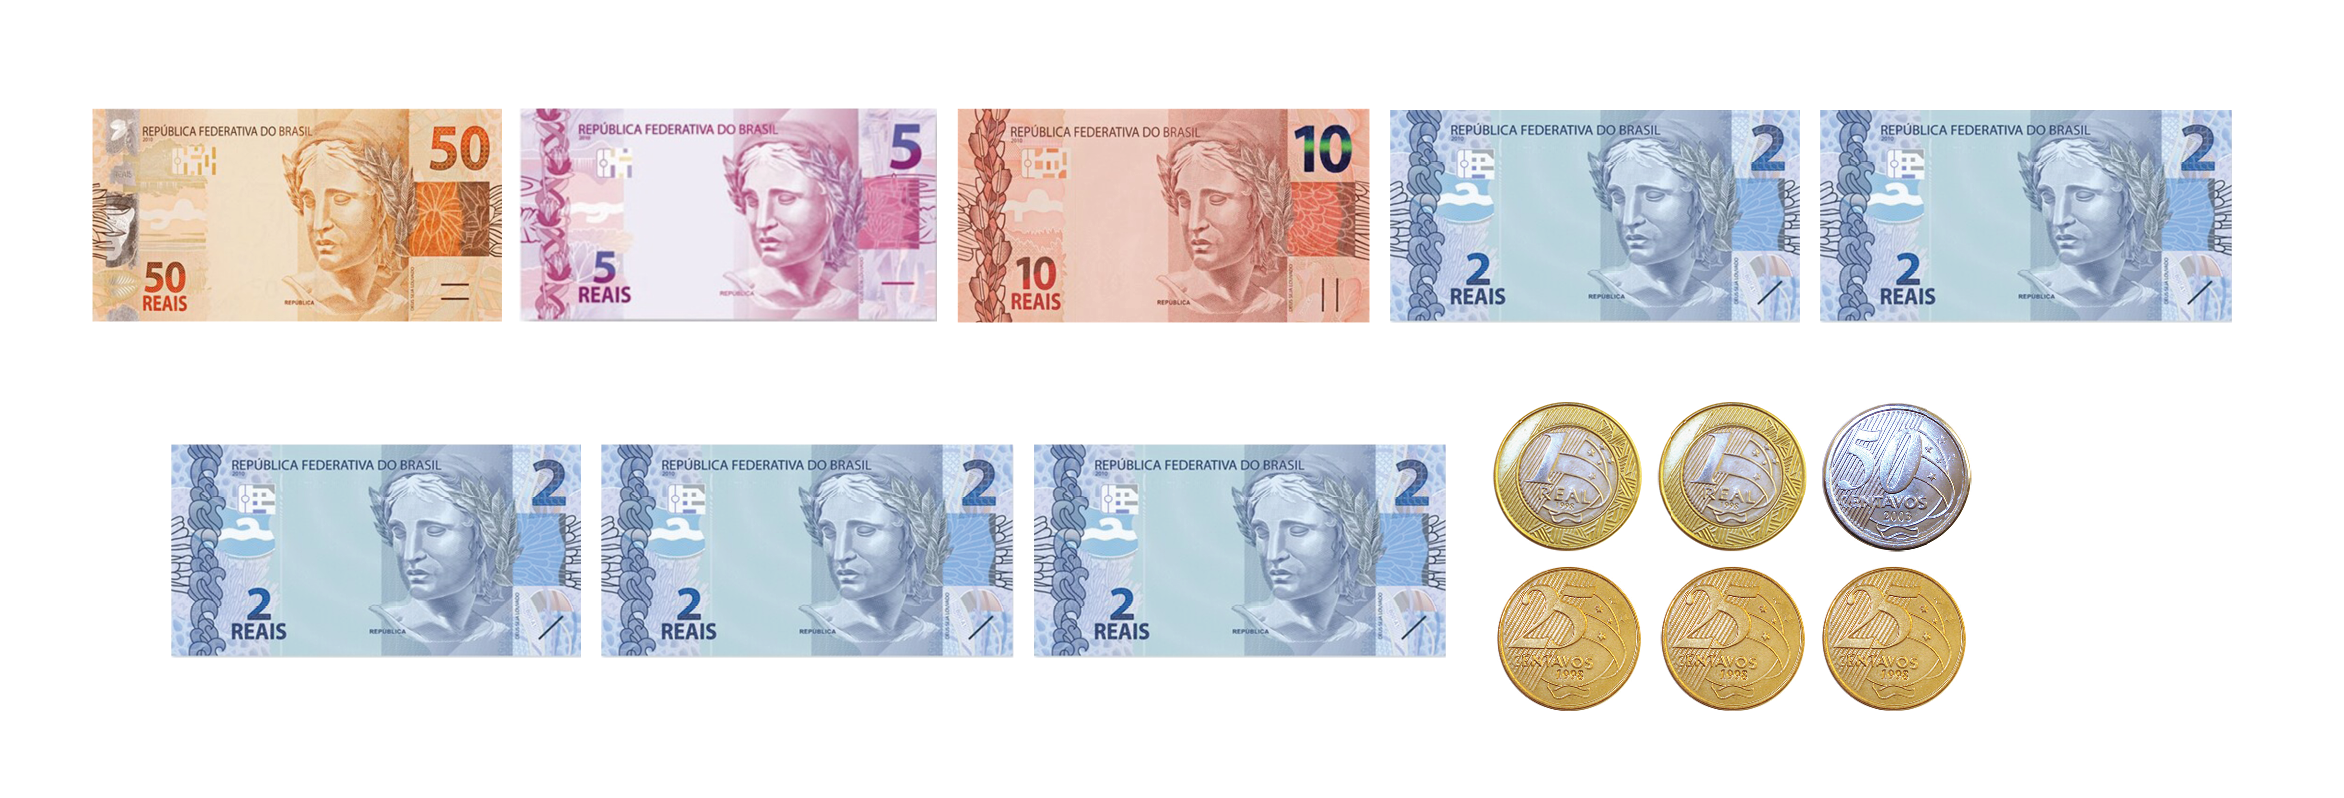
\includegraphics[width=\textwidth]{./media/image156.png}
\end{figure}

\begin{escolha}[itemsep=-5pt]
\item Boneca de 78 reais.

\item Casinha de 105 reais.

\item Patins de 96 reais.

\item Videogame de 500 reais.
\end{escolha}

\num{10} Luís comprou um patinete no valor de R\$249,00 e, para pagar, entregou
para a profissional que estava no caixa 3 notas de 100 reais. Quanto ela deve devolver de troco, em reais?

\begin{escolha}[itemsep=-5pt]
\item 48

\item 49

\item 50

\item 51
\end{escolha}

\num{11} Andressa lança sucessivamente um dado de seis lados, numerados de 1 a 6.
Indique a alternativa correta.

\begin{escolha}[itemsep=-5pt]
\item É pouco provável que seja sorteado um número ímpar em um lançamento.

\item É muito provável que se sorteie o número seis duas vezes consecutivas.

\item É possível que se sorteie o número oito.

\item É certo que se possa sortear um número maior que três.
\end{escolha}


\num{12} Lucas anotou a quantidade de rodas dos veículos estacionados na sua rua.
A tabela indica a quantidade de rodas em cada tipo de veículo. Marque a
alternativa que seja verdadeira.

\begin{figure}[H]
\centering
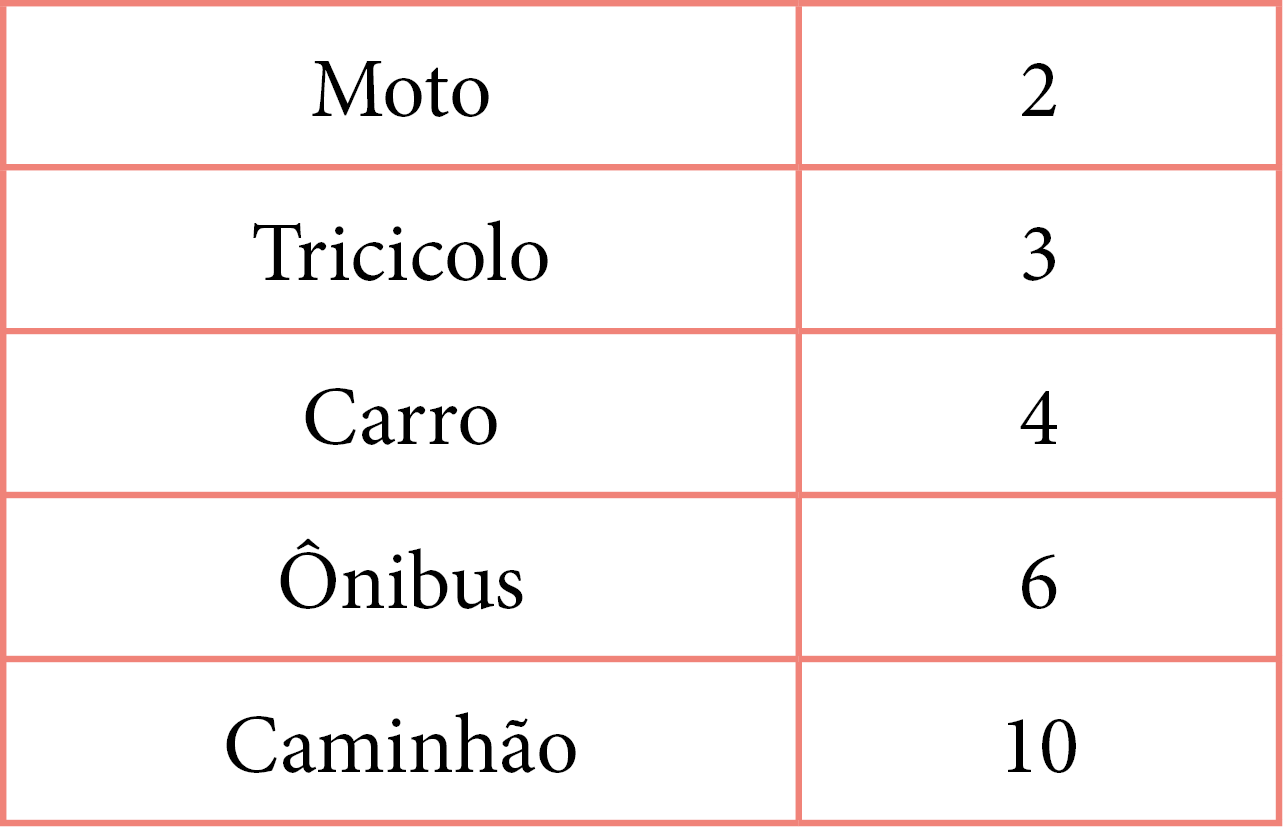
\includegraphics[width=.8\textwidth]{./media/image157.png}
\end{figure}

\begin{escolha}[itemsep=-5pt]
\item Duas motos possuem o mesmo número de rodas que um triciclo.

\item Dois carros possuem a quantidade de rodas de 3 motos.

\item Um caminhão possui a quantidade de rodas de um ônibus e um carro somados.

\item Um ônibus possui 3 rodas a mais que um carro.
\end{escolha}

\num{13} A professora Luana pergunta aos seus alunos do 2º ano quais as suas
brincadeiras prediletas e anota os votos dos estudantes. Segue o gráfico
contendo a relação dos votos.

\begin{figure}[H]
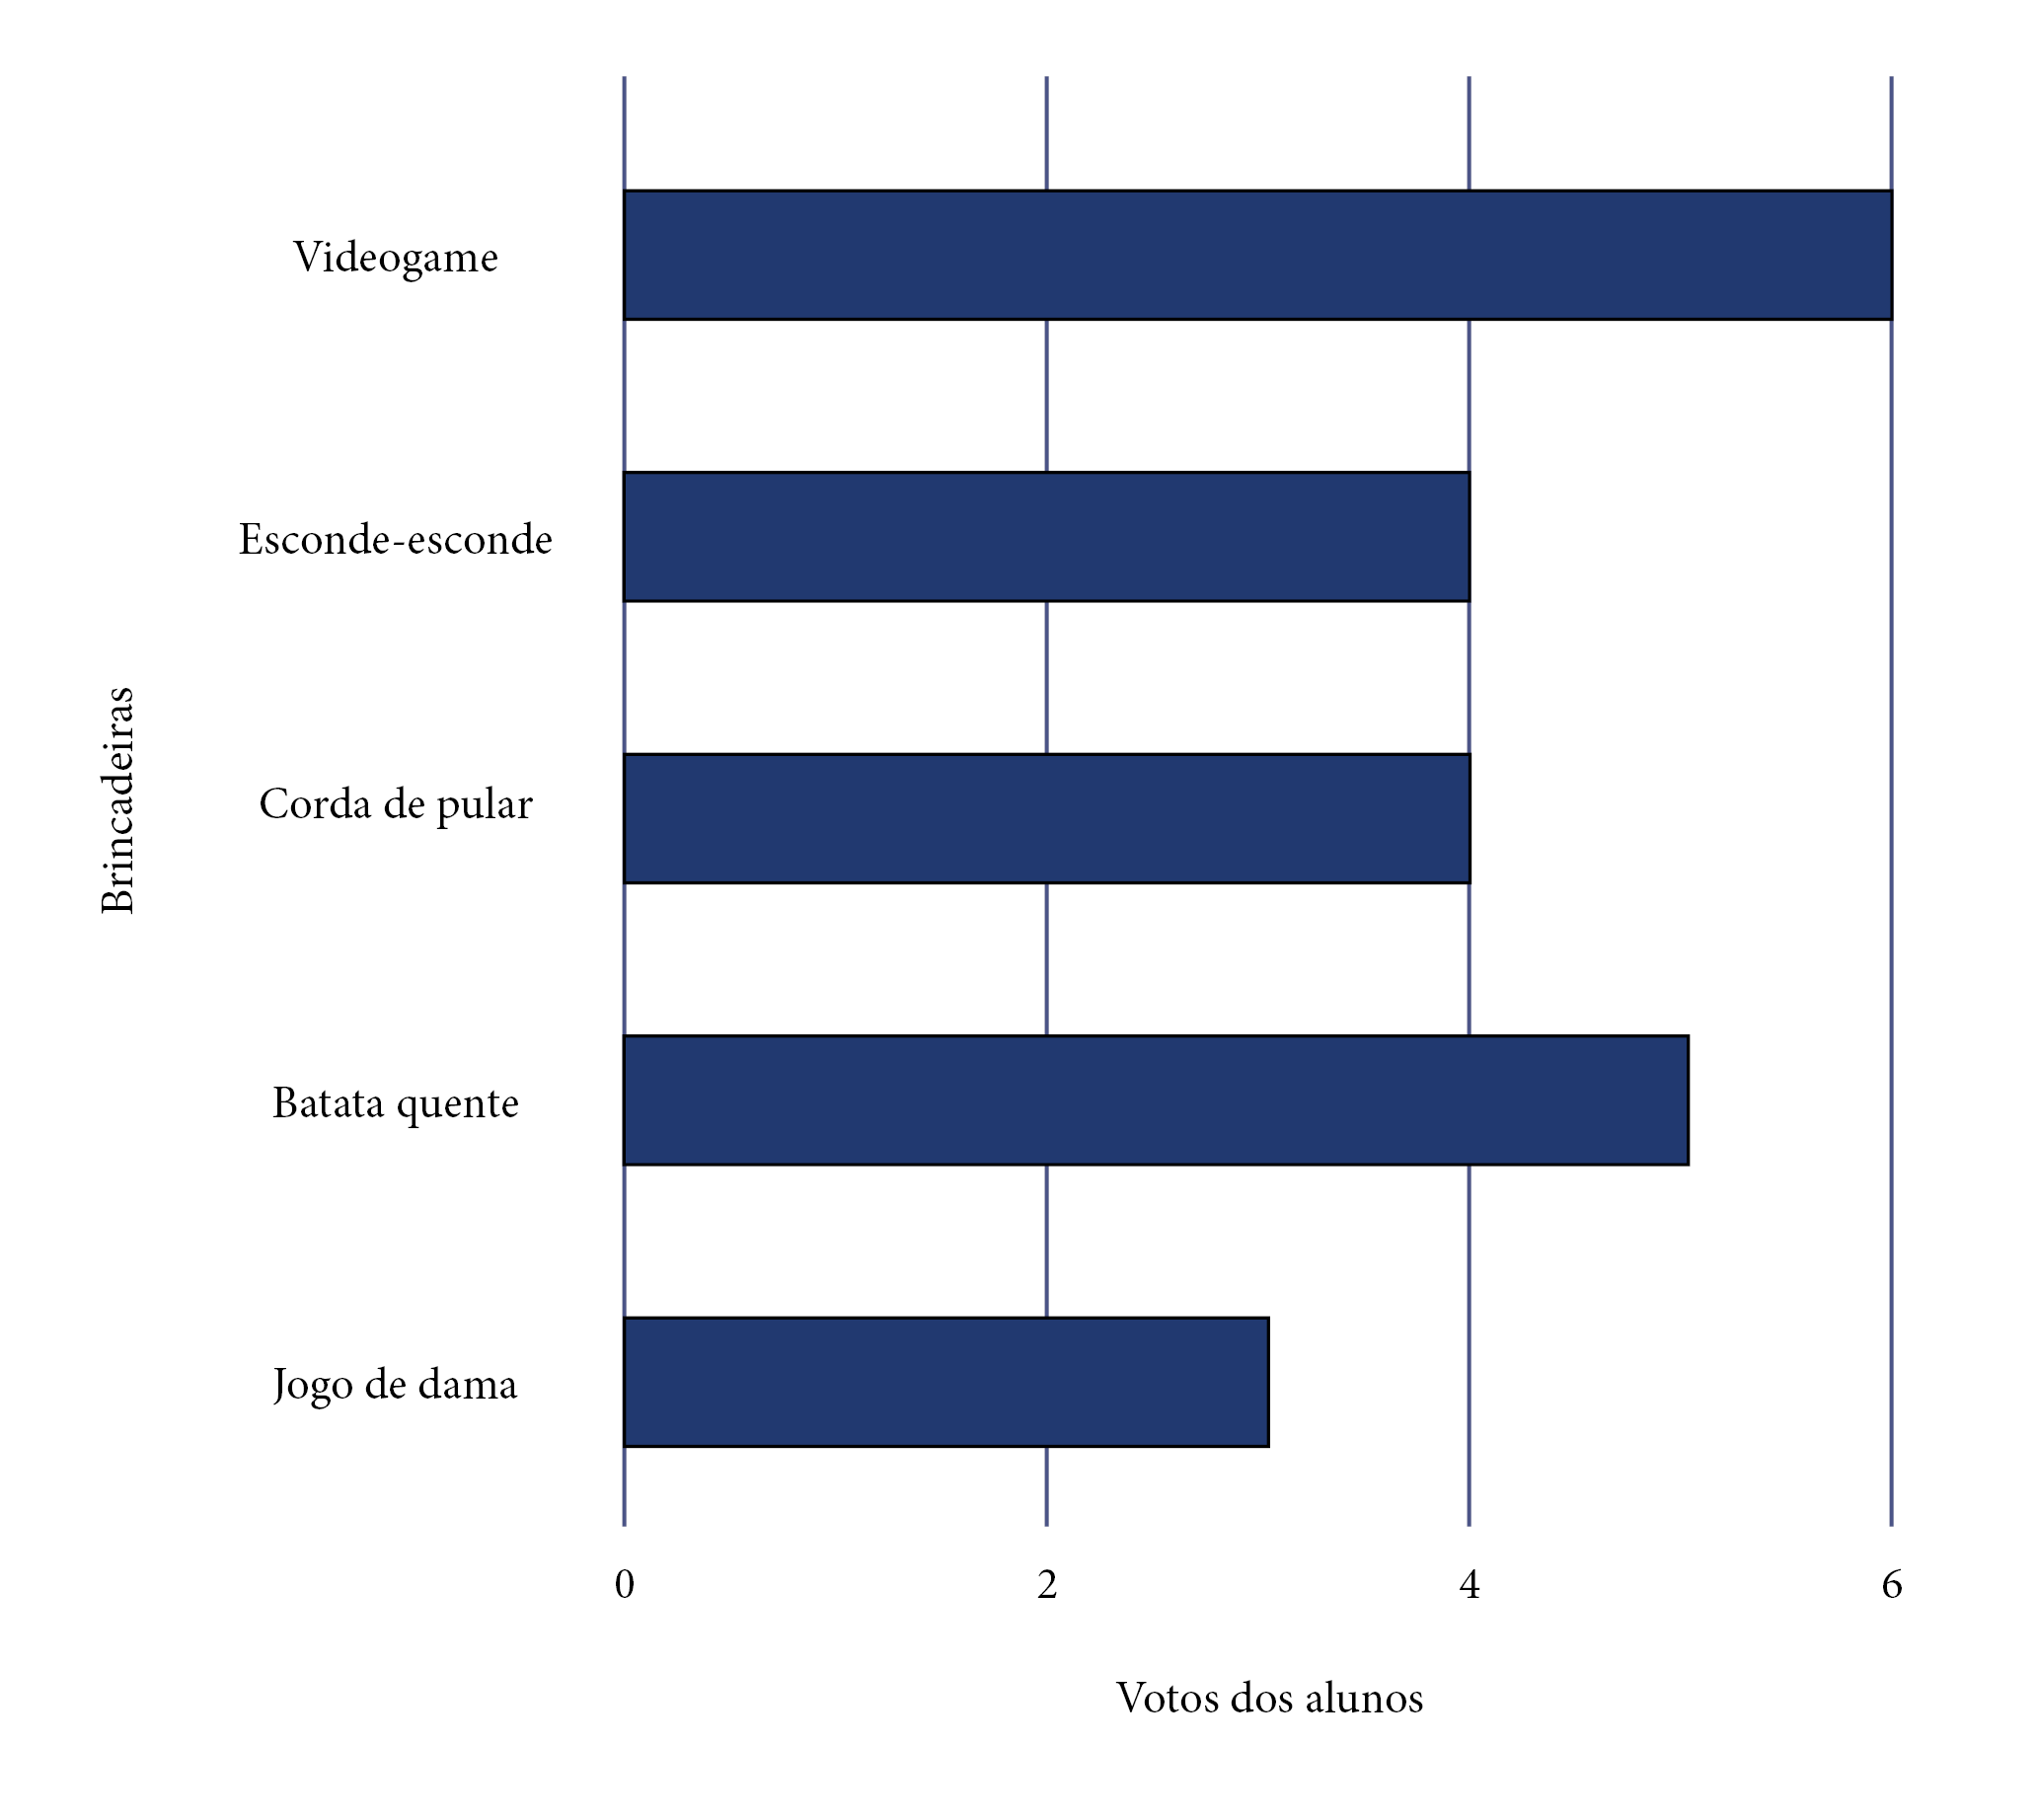
\includegraphics[width=\textwidth]{./media/image158.png}
\end{figure}

Indique a alternativa correta com relação ao gráfico.

\begin{escolha}[itemsep=-5pt]
\item A mesma quantidade de alunos prefere duas brincadeiras.

\item Batata-quente é a brincadeira preferida.

\item Não há uma brincadeira preferida entre os alunos.

\item O jogo de damas é o preferido.
\end{escolha}

\num{14} A avó de Cristina preparou torradinhas temperadas para o café da manhã.
Mas, como sua assadeira é pequena, só cabem 9 torradinhas de cada vez.
Considerando que ela teve de levar sua assadeira ao forno 5 vezes,
quantas torradinhas a vovó assou ao todo?

\begin{figure}[H]
\centering
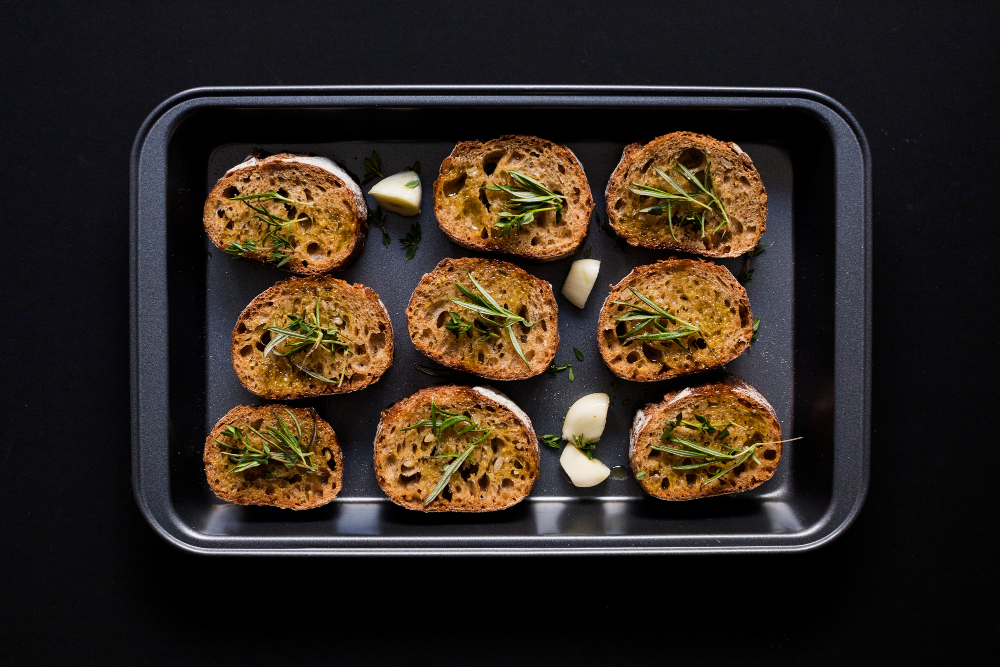
\includegraphics[width=.5\textwidth]{./media/image159.png}
\end{figure}

\begin{escolha}[itemsep=-5pt]
\item 9

\item 27

\item 45

\item 54
\end{escolha}

\num{15} Dona Cida fez 150 queijos que foram distribuídos para mercearias da cidade, sendo que cada mercearia recebeu 10 queijos. Quantas mercearias receberam os queijos de Dona
Cida para revenda?

\begin{escolha}[itemsep=-5pt]
\item 10

\item 15

\item 25

\item 30
\end{escolha}
